\section{Signal Kinematic Distributions }
\label{app:signal-dist}

%%\paragraph{}
This is a quick check of the signal region kinematic distributions; it is compared with data from $0b$ Tag signal region, as a rough estimate of possible QCD background shape. Figures ~\ref{fig:app-signal-jj}, ~\ref{fig:app-signal-leadHCand}, ~\ref{fig:app-signal-sublHCand}, are the normalized distributions. All plots shown are RSG samples with $c=1.0$. Figure ~\ref{fig:app-signal-mhh} shows the signal sample distribution on the mHH plane.


\begin{figure*}[htbp!]
\begin{center}
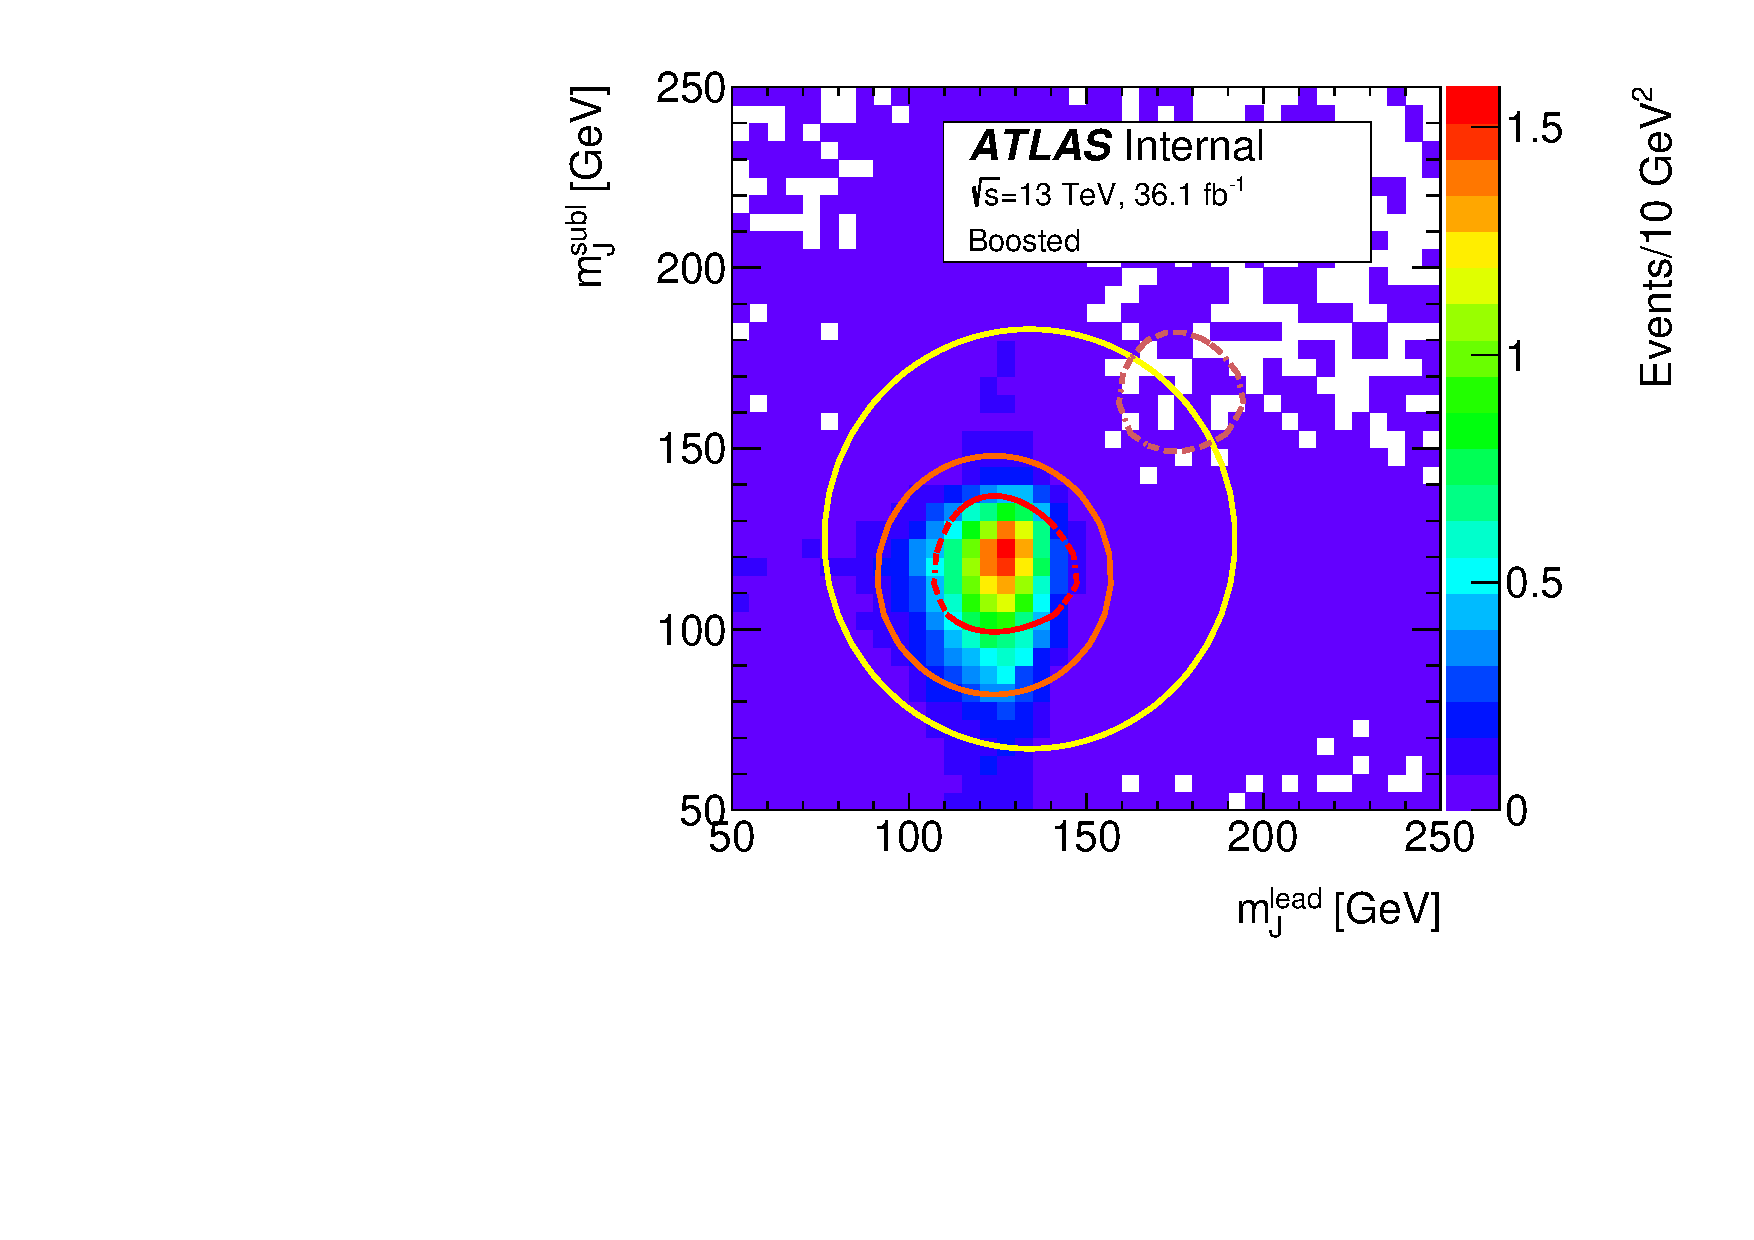
\includegraphics[width=0.32\textwidth,angle=-90]{figures/boosted/Truth/Sig_1200_AllTag_Incl_mH0H1.pdf}
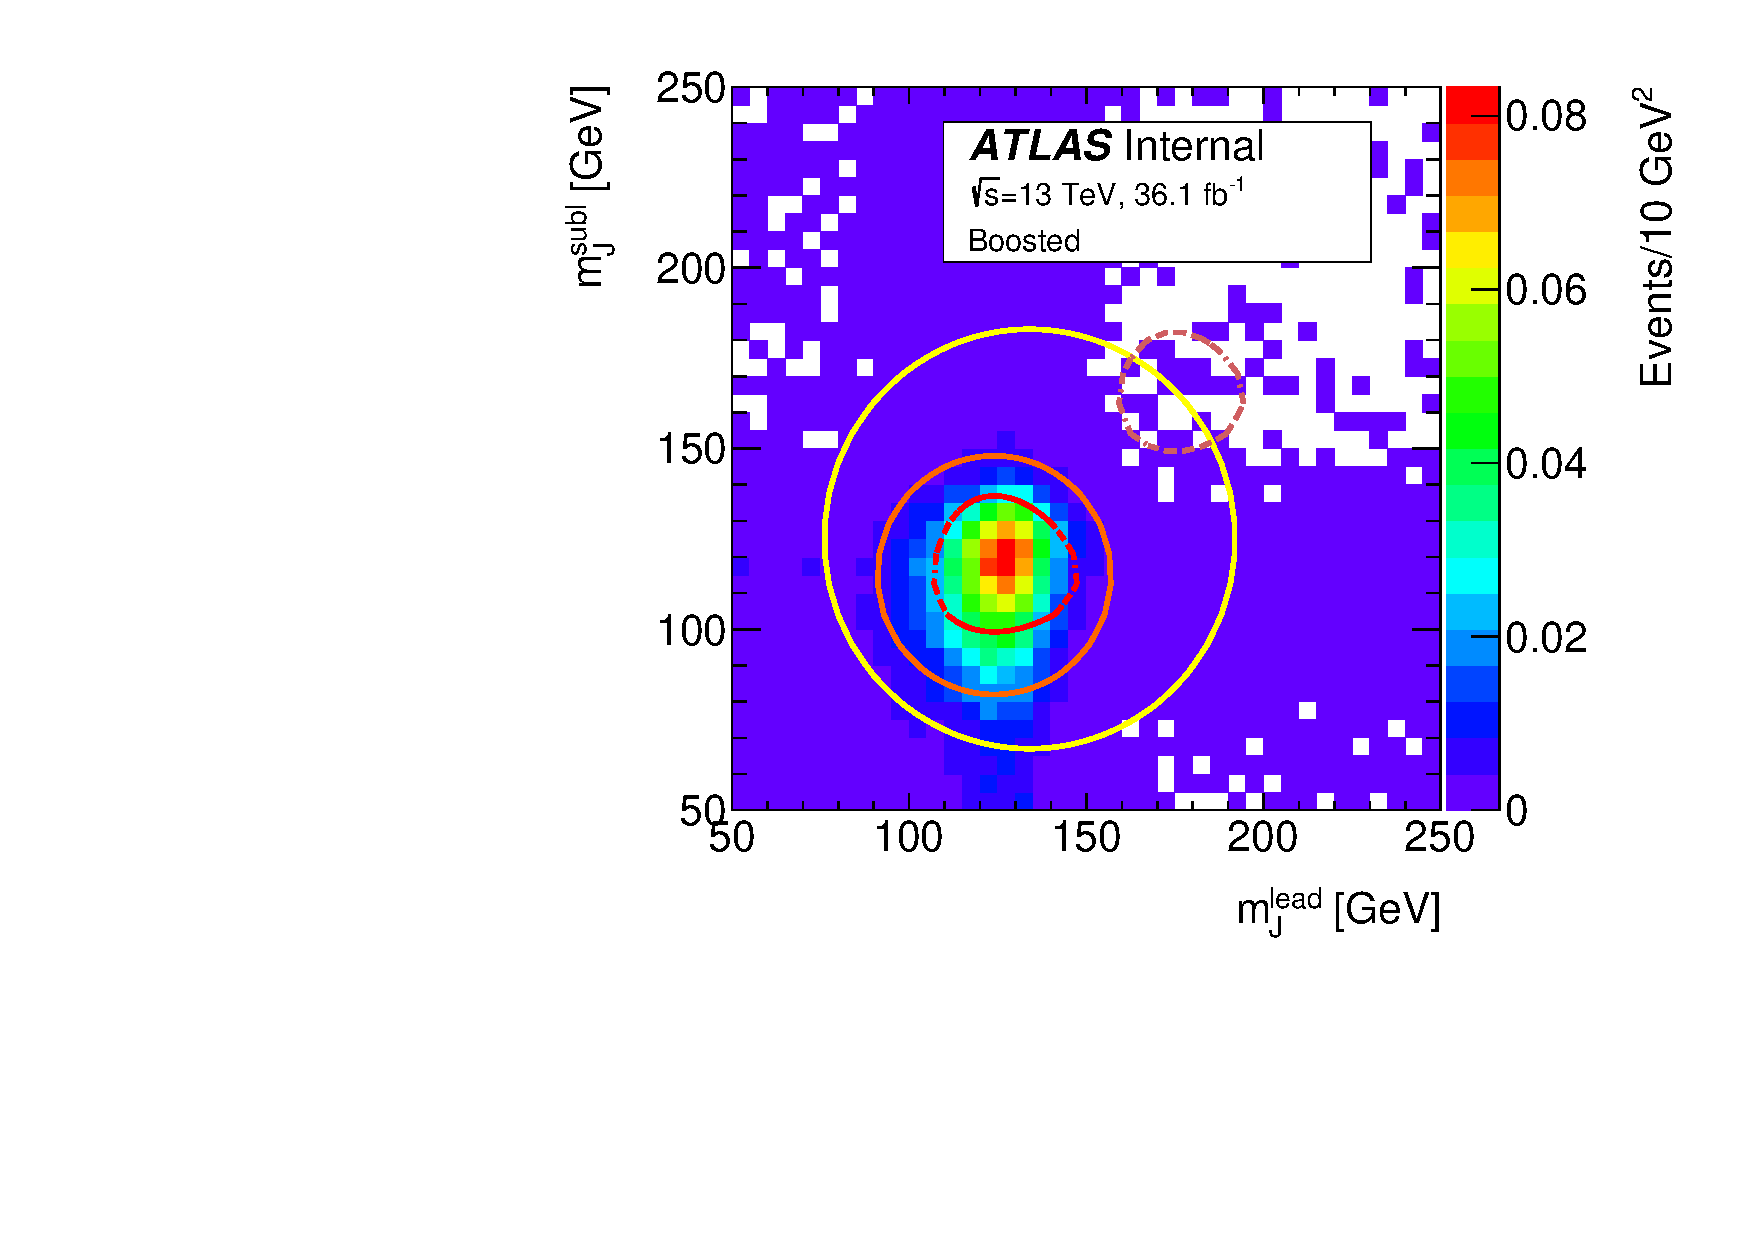
\includegraphics[width=0.32\textwidth,angle=-90]{figures/boosted/Truth/Sig_2000_AllTag_Incl_mH0H1.pdf}
\caption{For RSG $c=1.0$ samples, number of events as a funciton of leading Higgs candidate mass and subleading Higgs candidate mass, for 1.2 TeV(left) signal and 2.0 TeV(right) signal samples.}
\label{fig:app-signal-mhh}
\end{center}
\end{figure*}

\begin{figure*}[htbp!]
\begin{center}
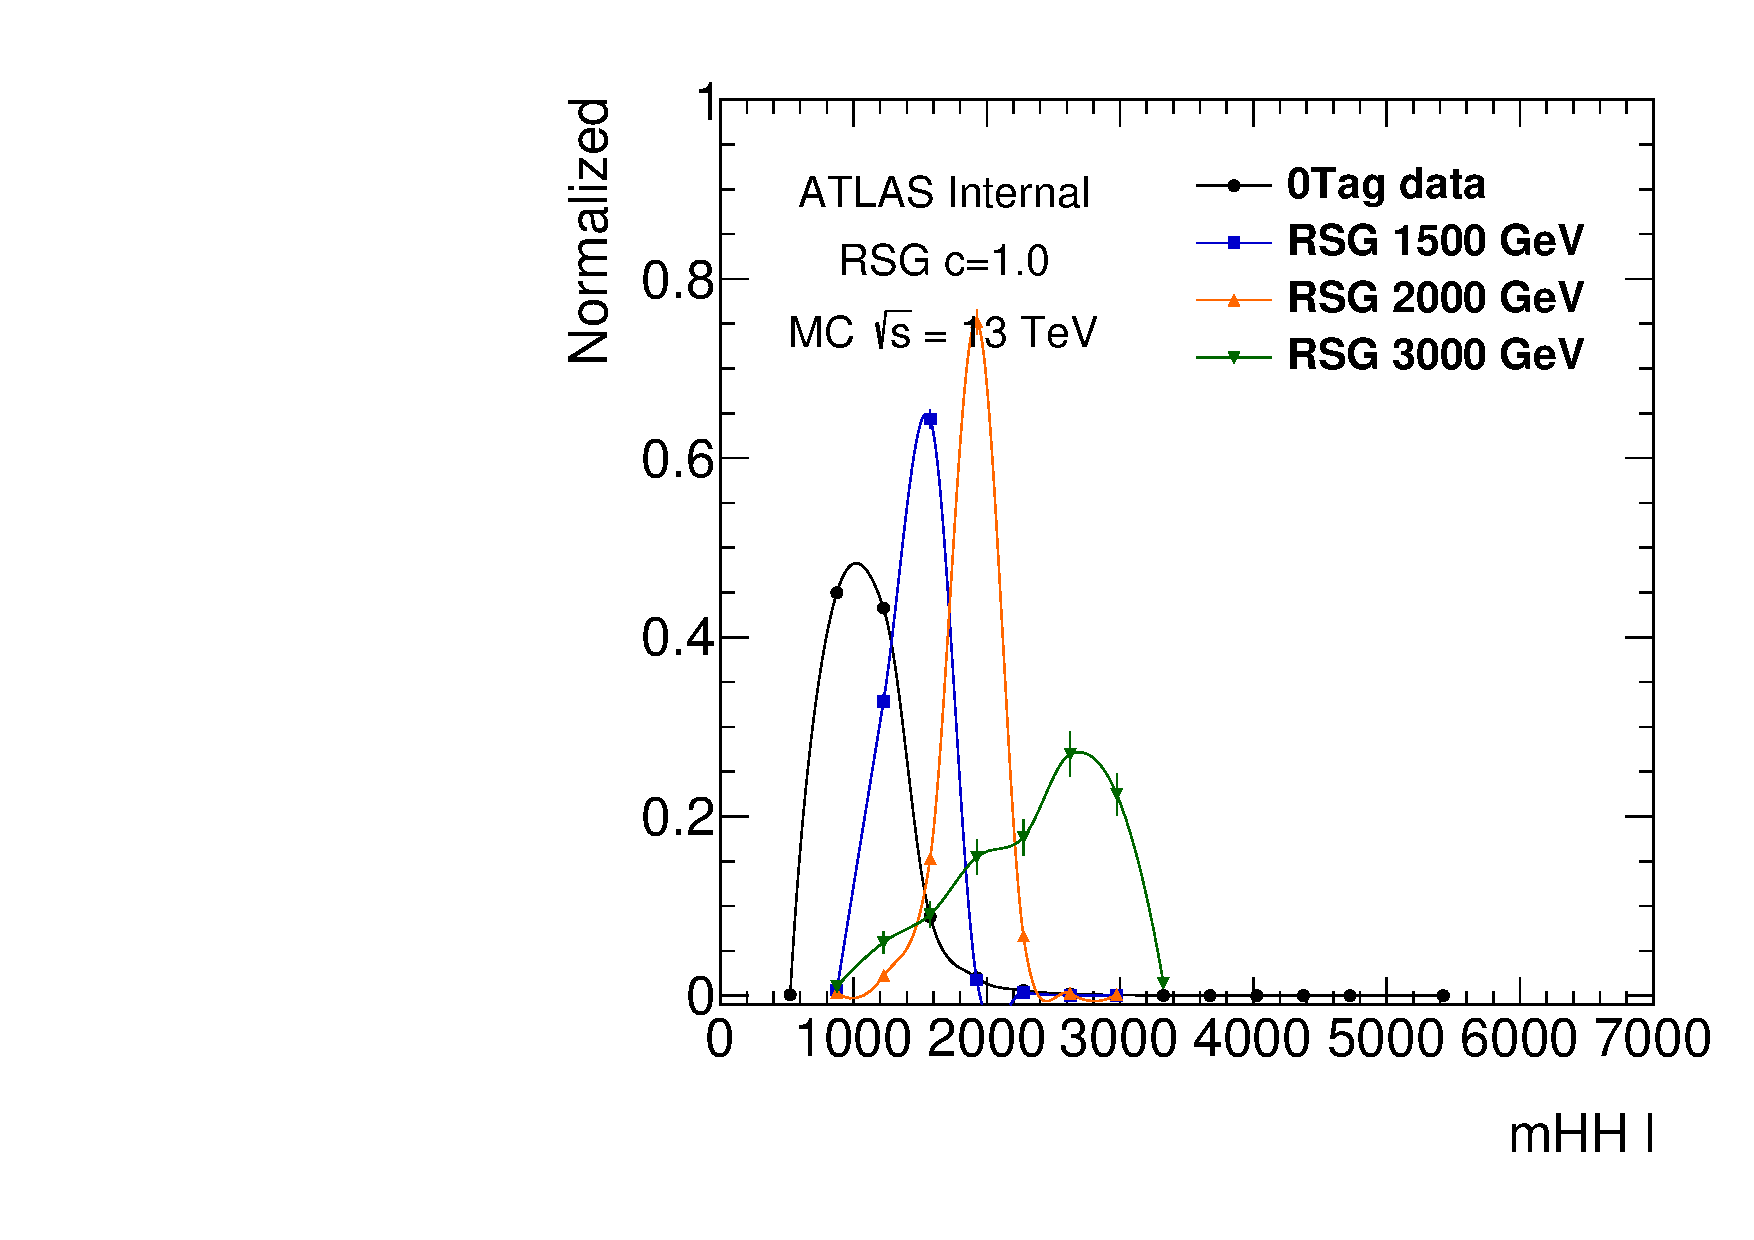
\includegraphics[width=0.32\textwidth,angle=-90]{figures/boosted/Truth/Moriond_comp_0_FourTag_Signal_mHH_l.pdf}
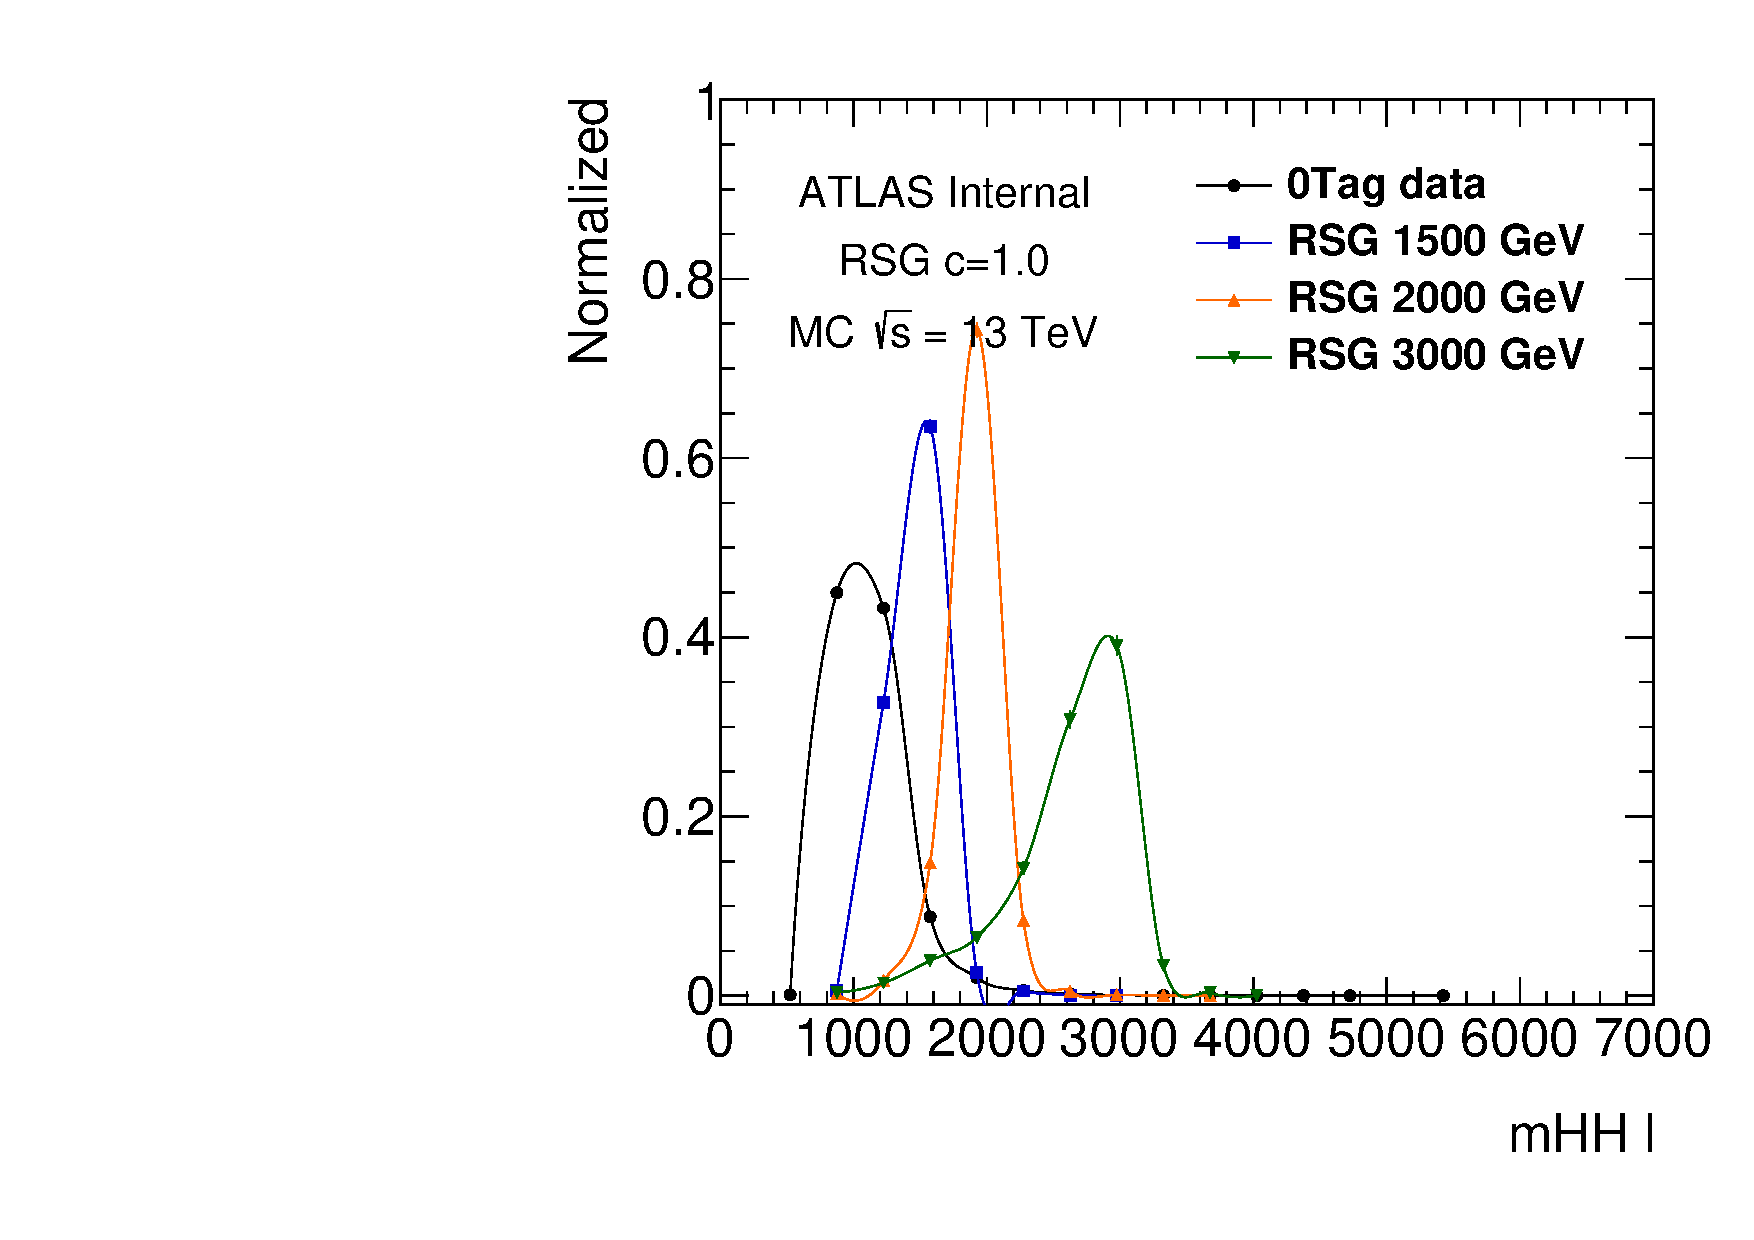
\includegraphics[width=0.32\textwidth,angle=-90]{figures/boosted/Truth/Moriond_comp_0_ThreeTag_Signal_mHH_l.pdf}
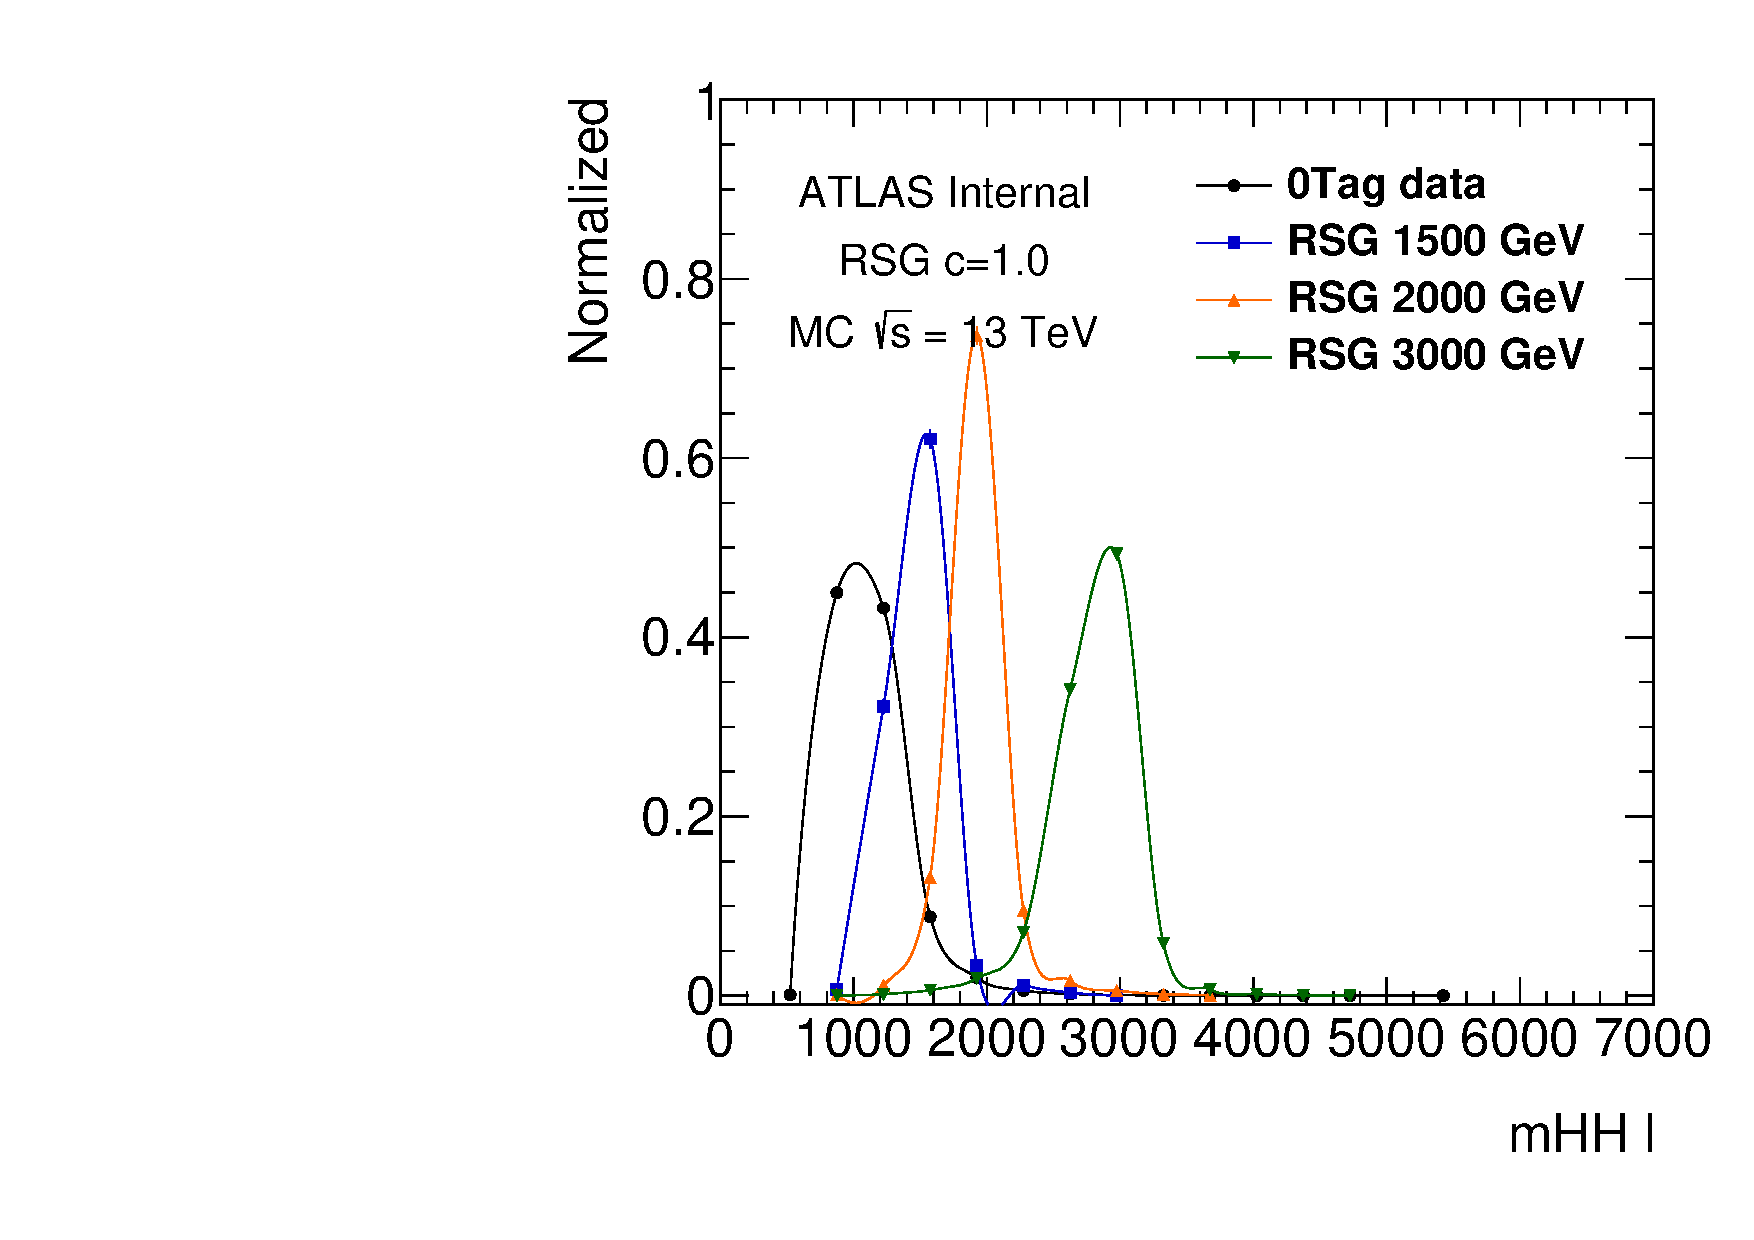
\includegraphics[width=0.32\textwidth,angle=-90]{figures/boosted/Truth/Moriond_comp_0_TwoTag_split_Signal_mHH_l.pdf}\\
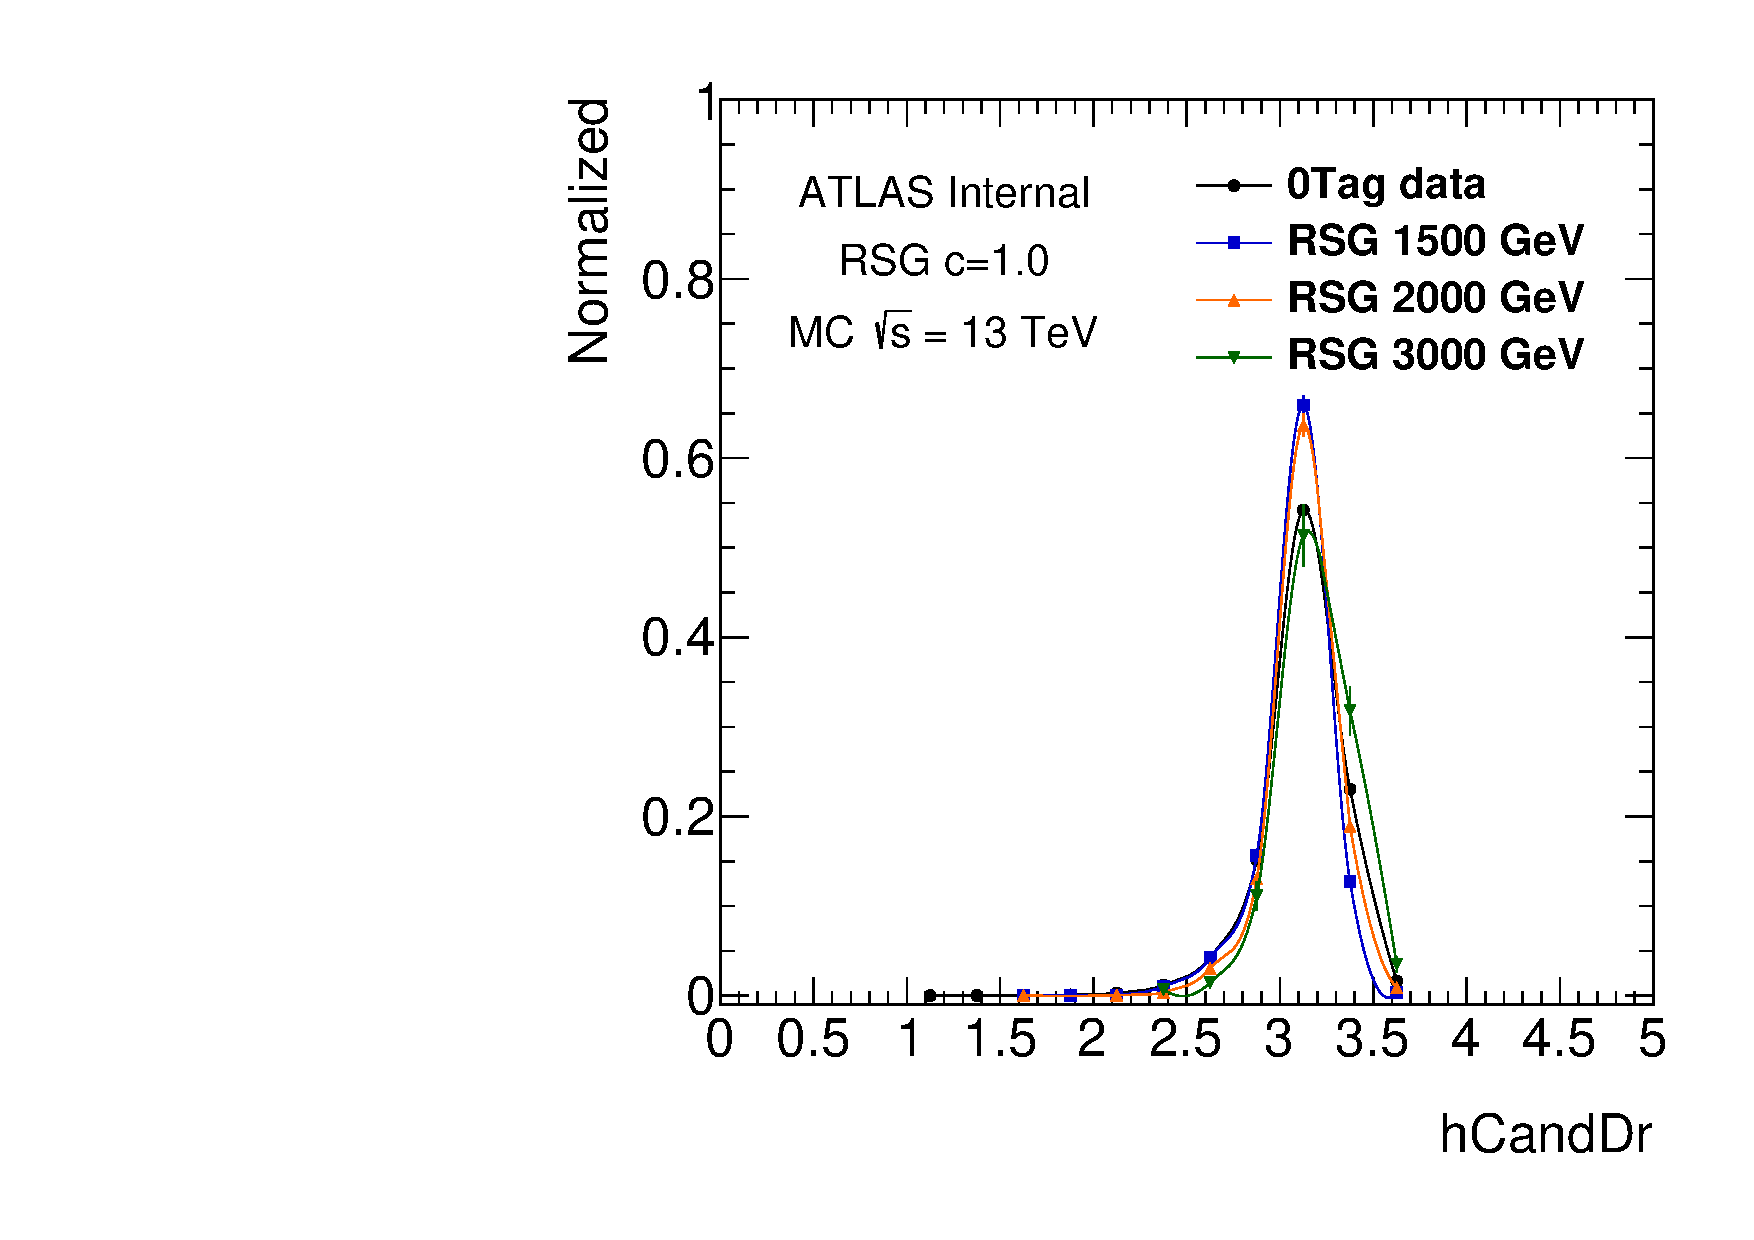
\includegraphics[width=0.32\textwidth,angle=-90]{figures/boosted/Truth/Moriond_comp_0_FourTag_Signal_hCandDr.pdf}
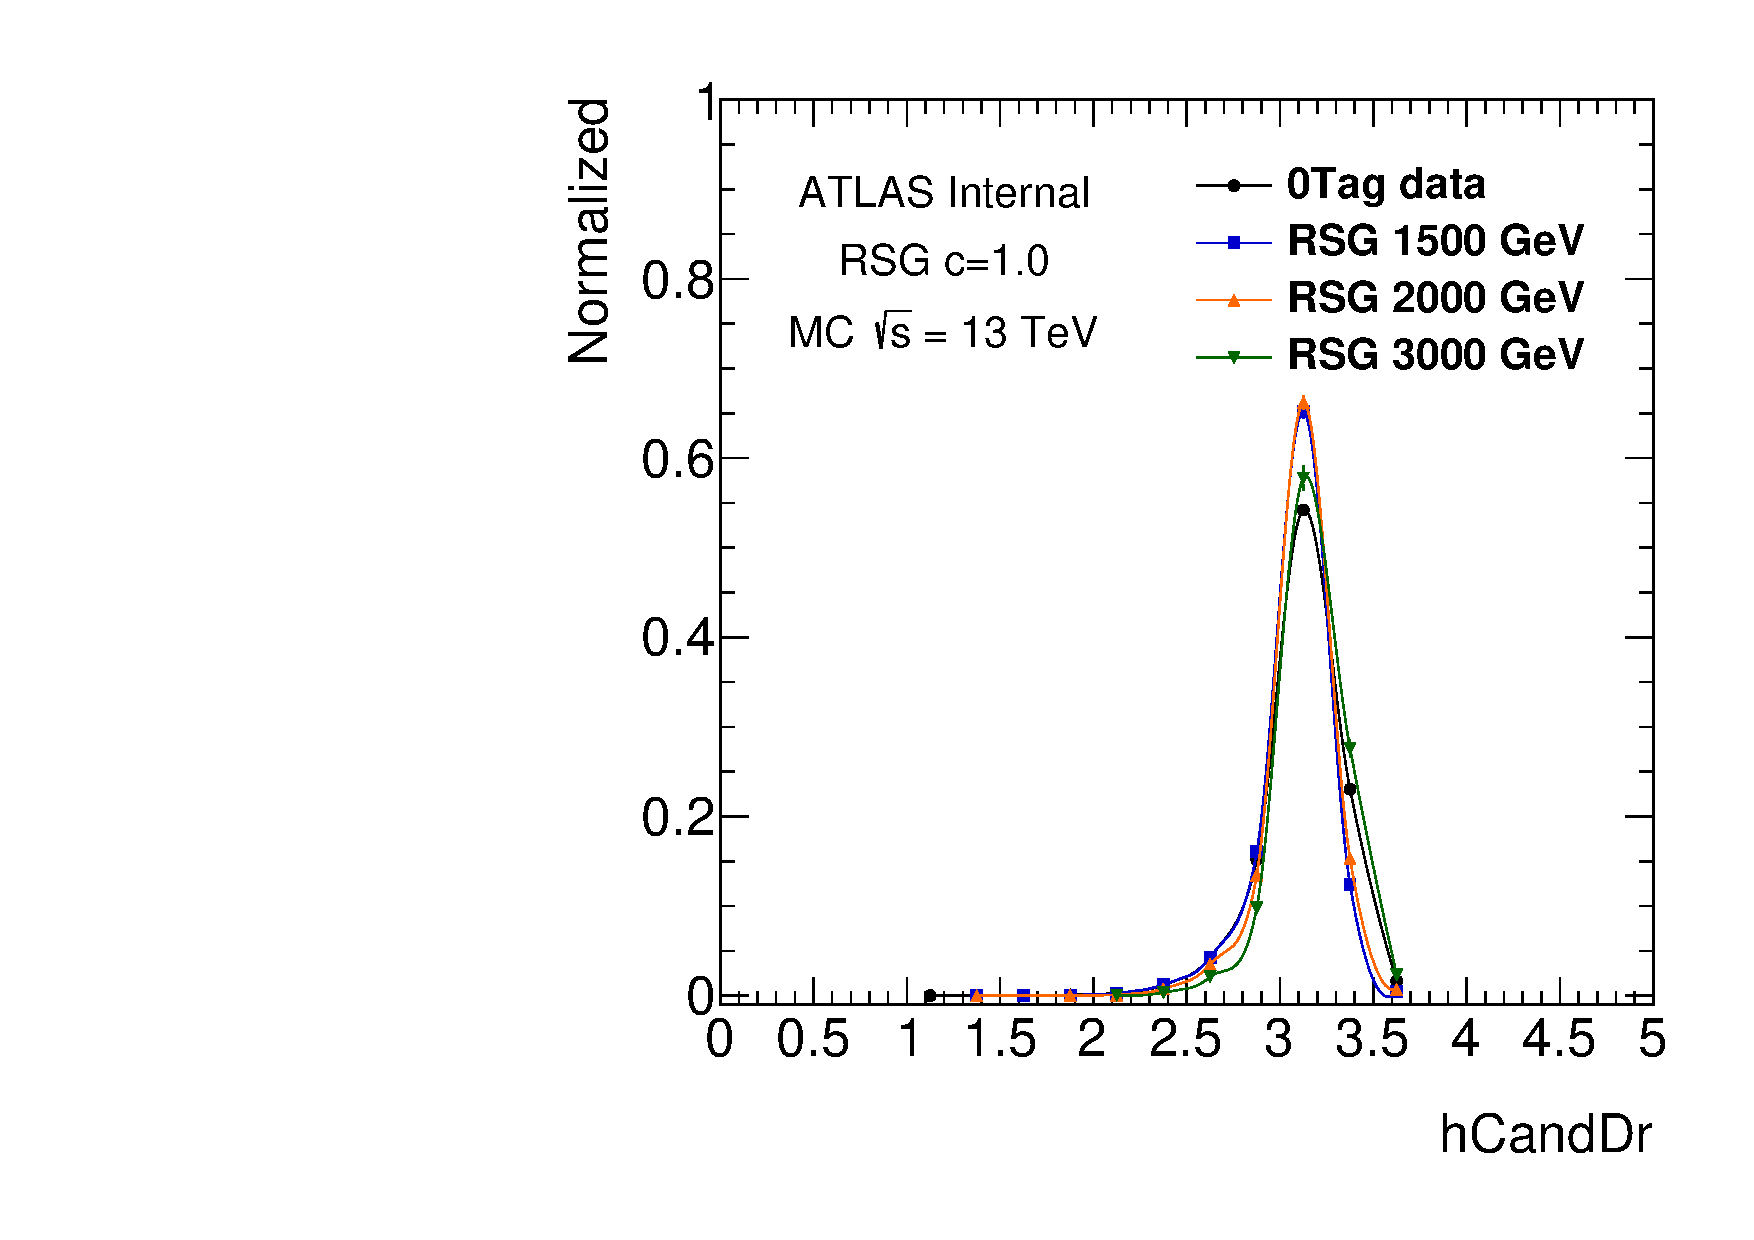
\includegraphics[width=0.32\textwidth,angle=-90]{figures/boosted/Truth/Moriond_comp_0_ThreeTag_Signal_hCandDr.pdf}
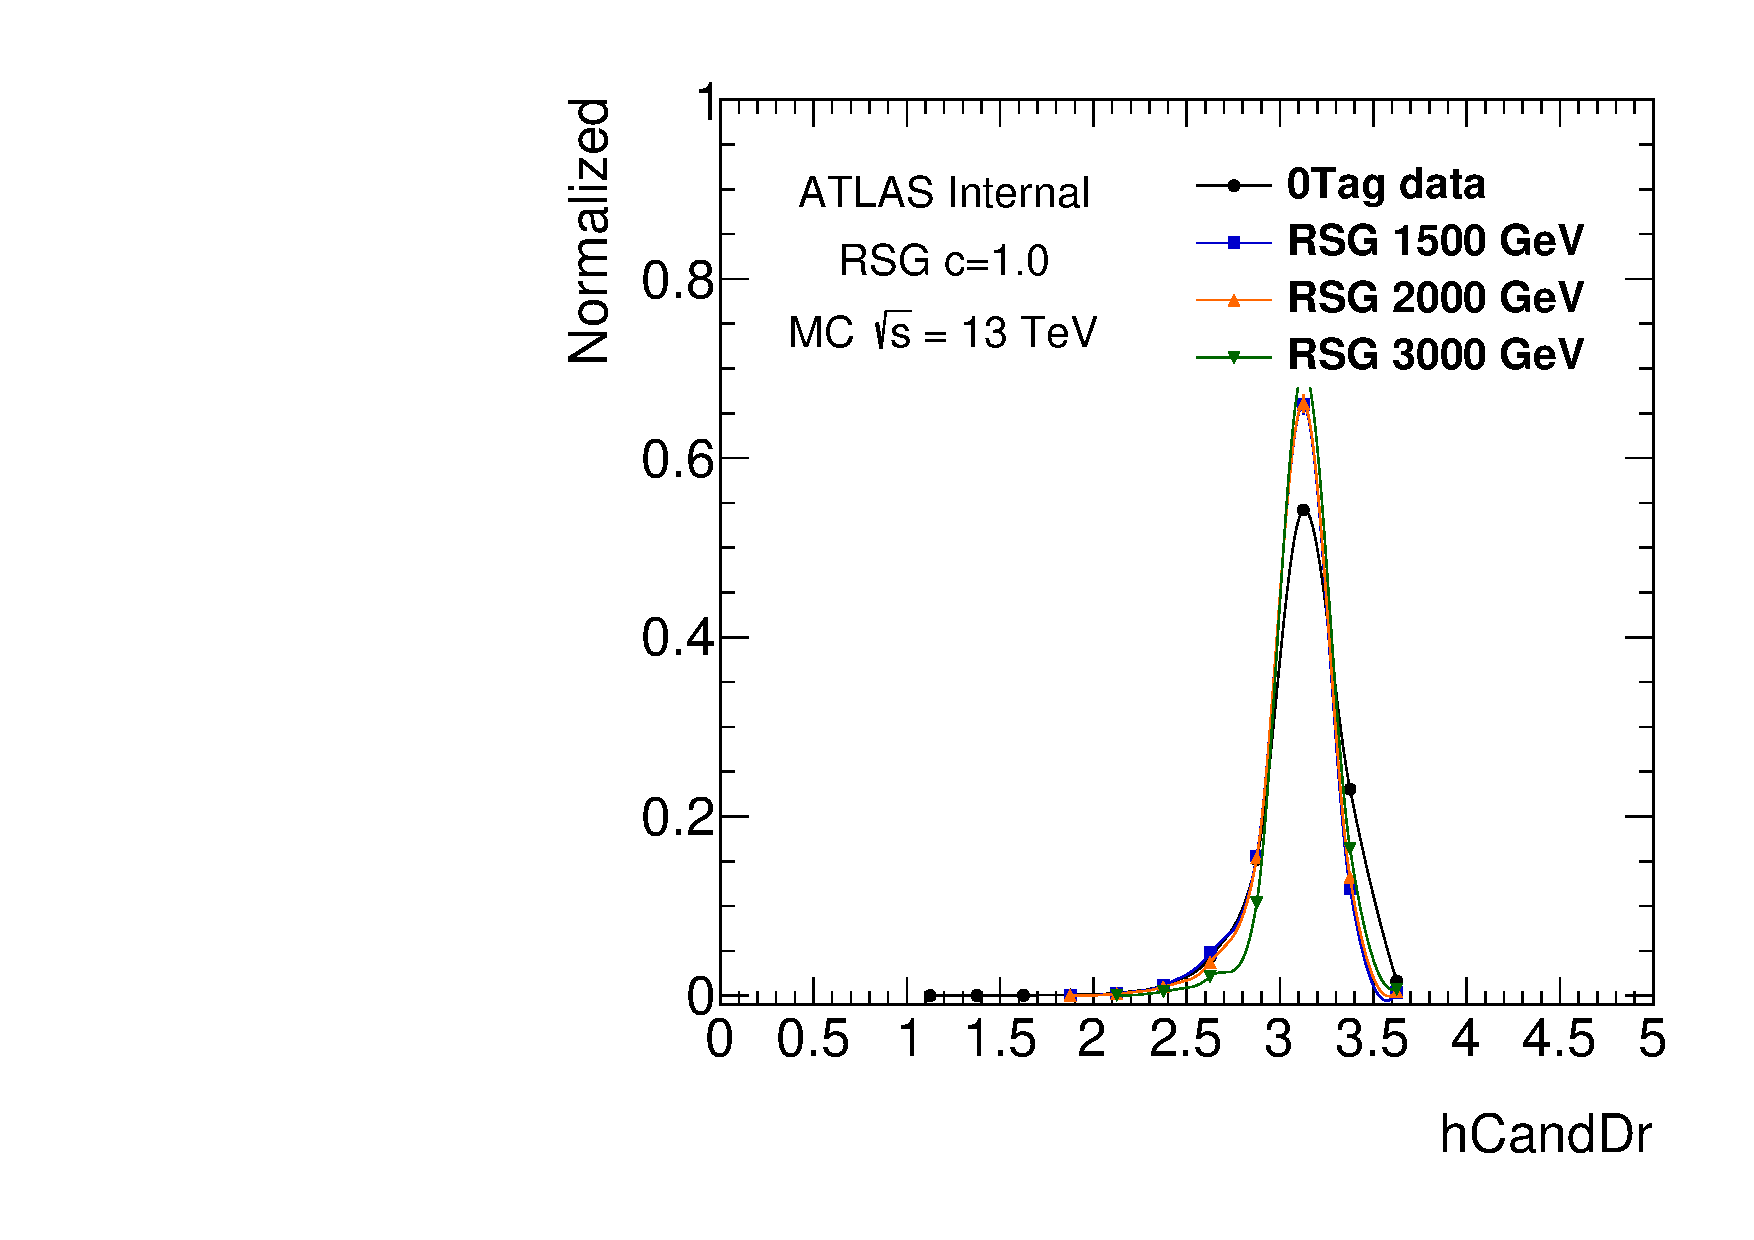
\includegraphics[width=0.32\textwidth,angle=-90]{figures/boosted/Truth/Moriond_comp_0_TwoTag_split_Signal_hCandDr.pdf}\\
\caption{For RSG $c=1.0$ samples, the dijet mass distributions and $\Delta R$ between the two large-\R jets. The left column is $4b$, the middle column is $3b$, and the right column is $2bs$.}
\label{fig:app-signal-jj}
\end{center}
\end{figure*}


\begin{figure*}[htbp!]
\begin{center}
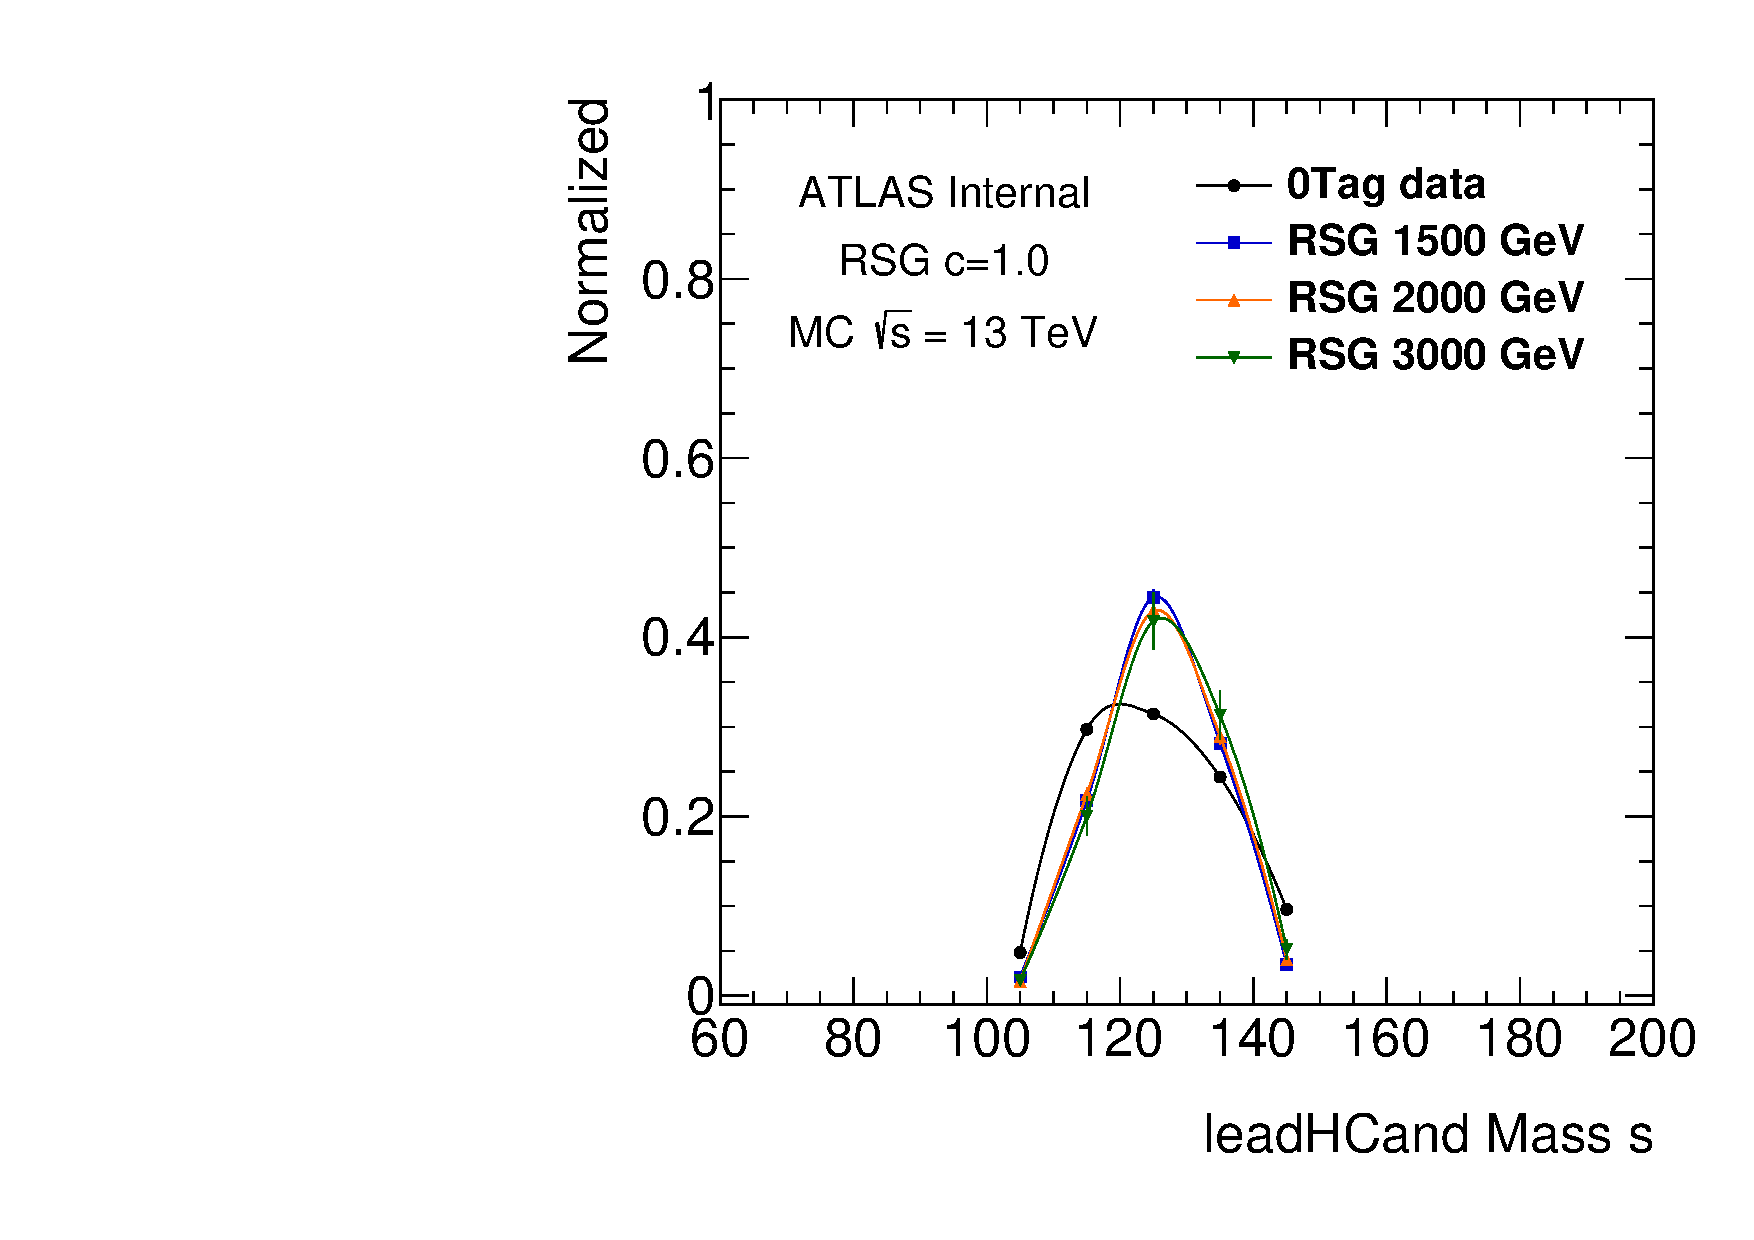
\includegraphics[width=0.32\textwidth,angle=-90]{figures/boosted/Truth/Moriond_comp_0_FourTag_Signal_leadHCand_Mass_s.pdf}
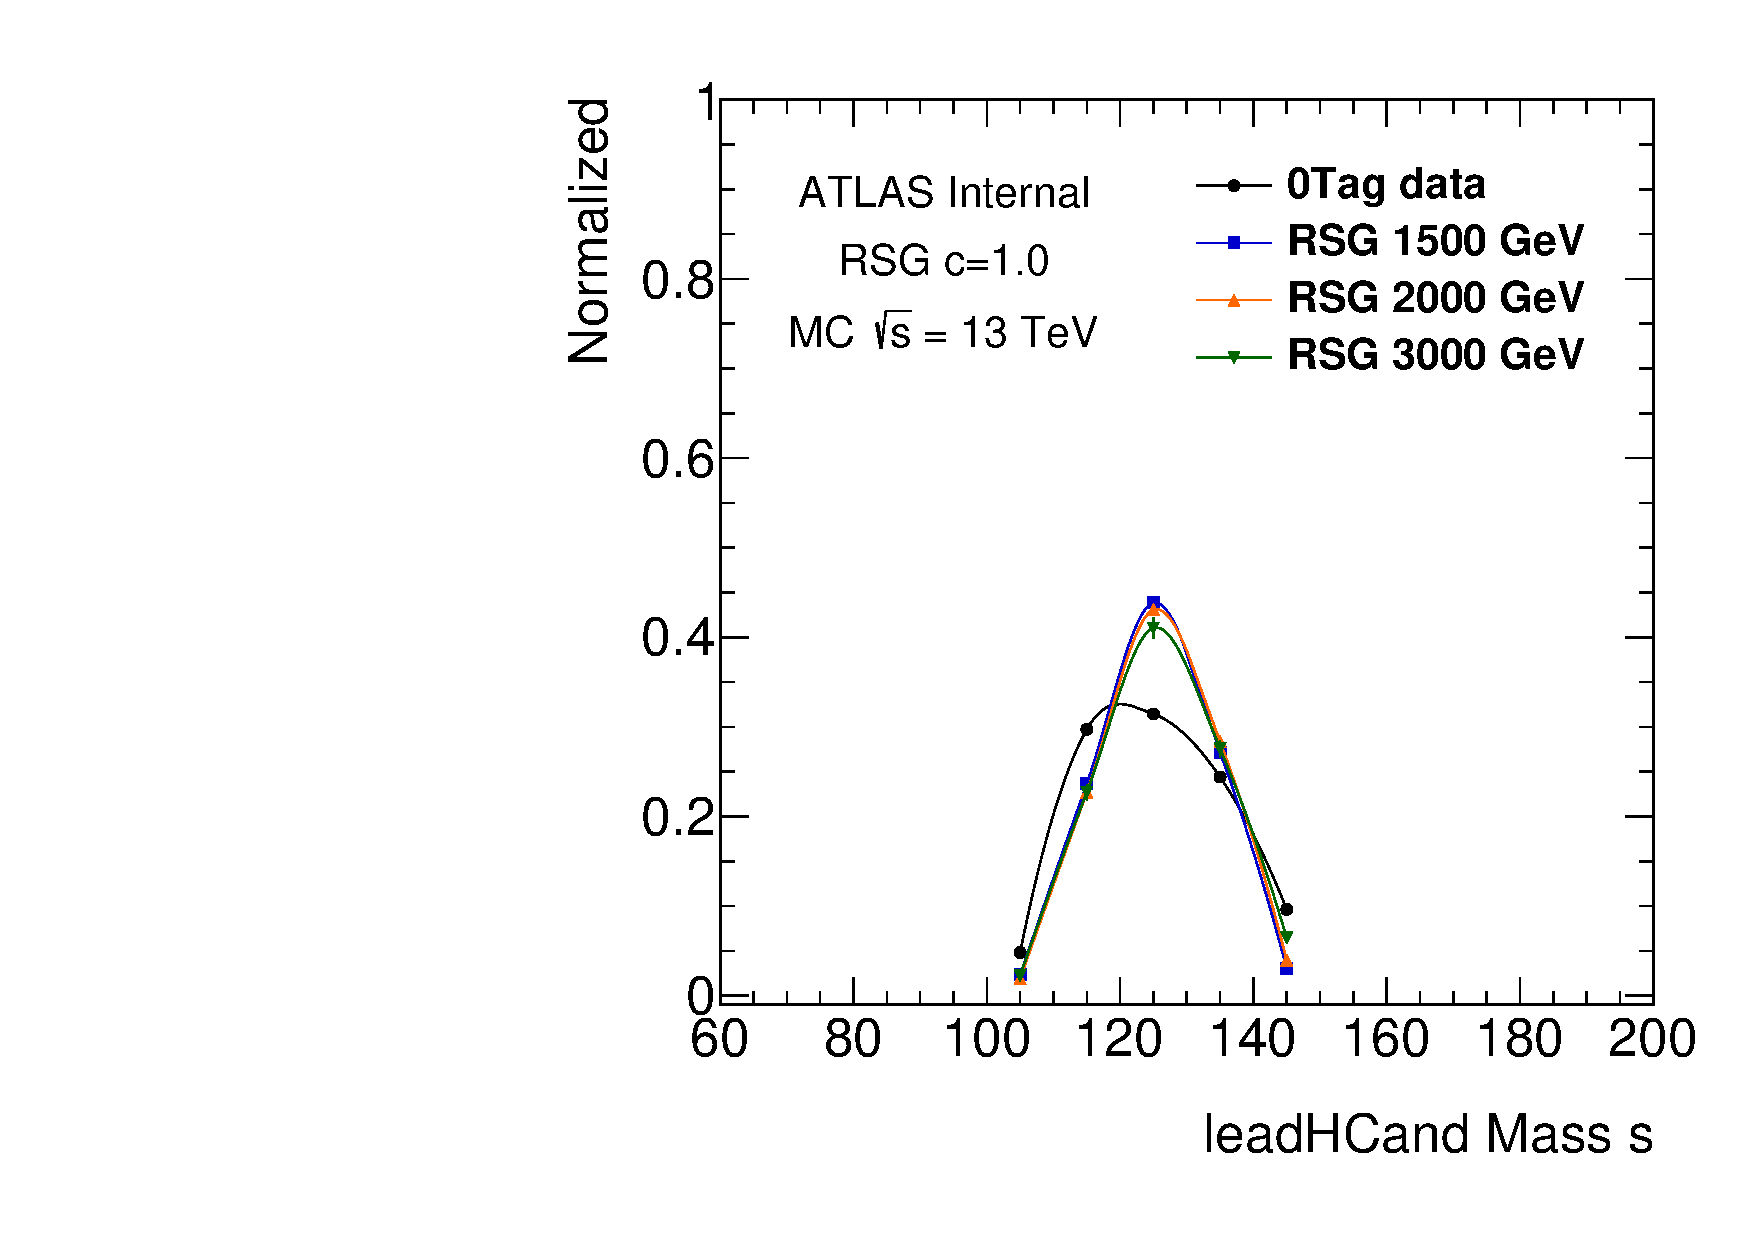
\includegraphics[width=0.32\textwidth,angle=-90]{figures/boosted/Truth/Moriond_comp_0_ThreeTag_Signal_leadHCand_Mass_s.pdf}
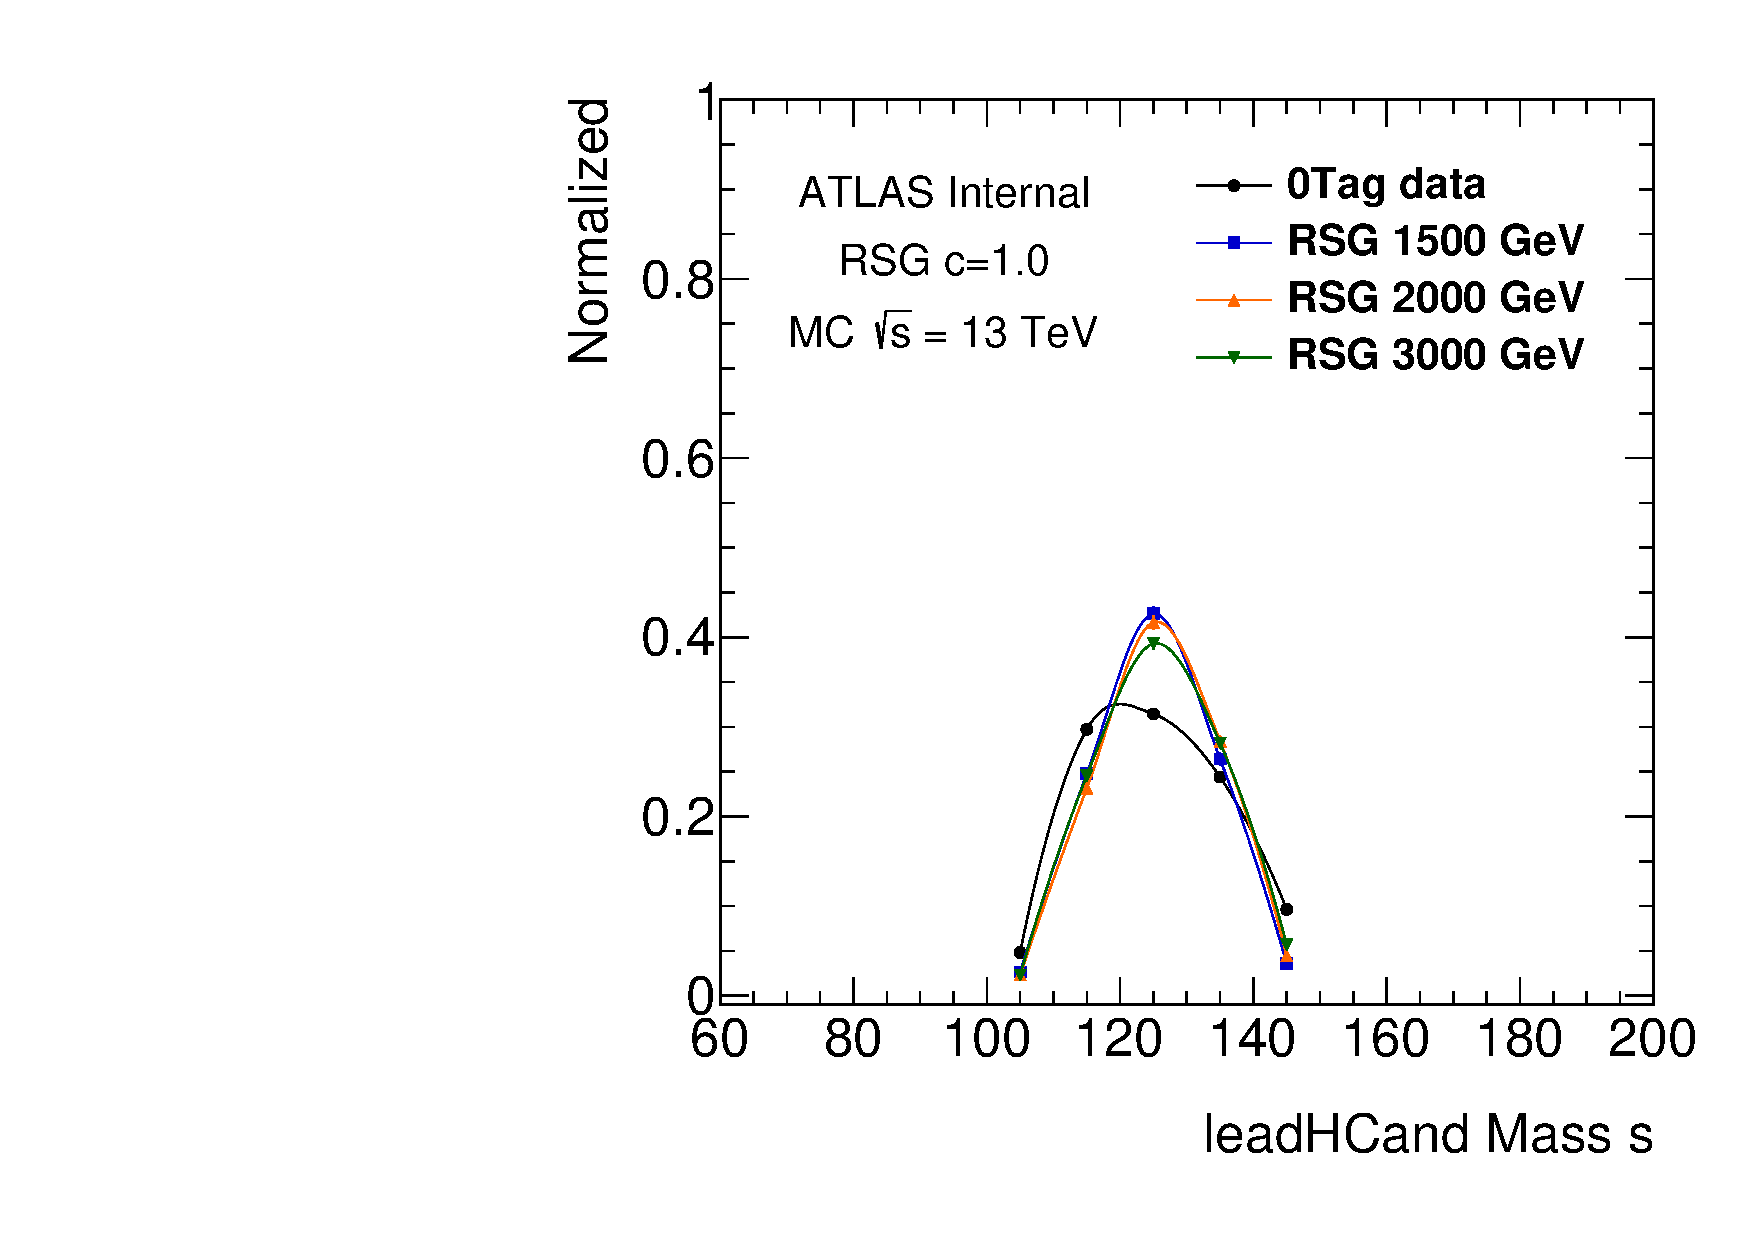
\includegraphics[width=0.32\textwidth,angle=-90]{figures/boosted/Truth/Moriond_comp_0_TwoTag_split_Signal_leadHCand_Mass_s.pdf}\\
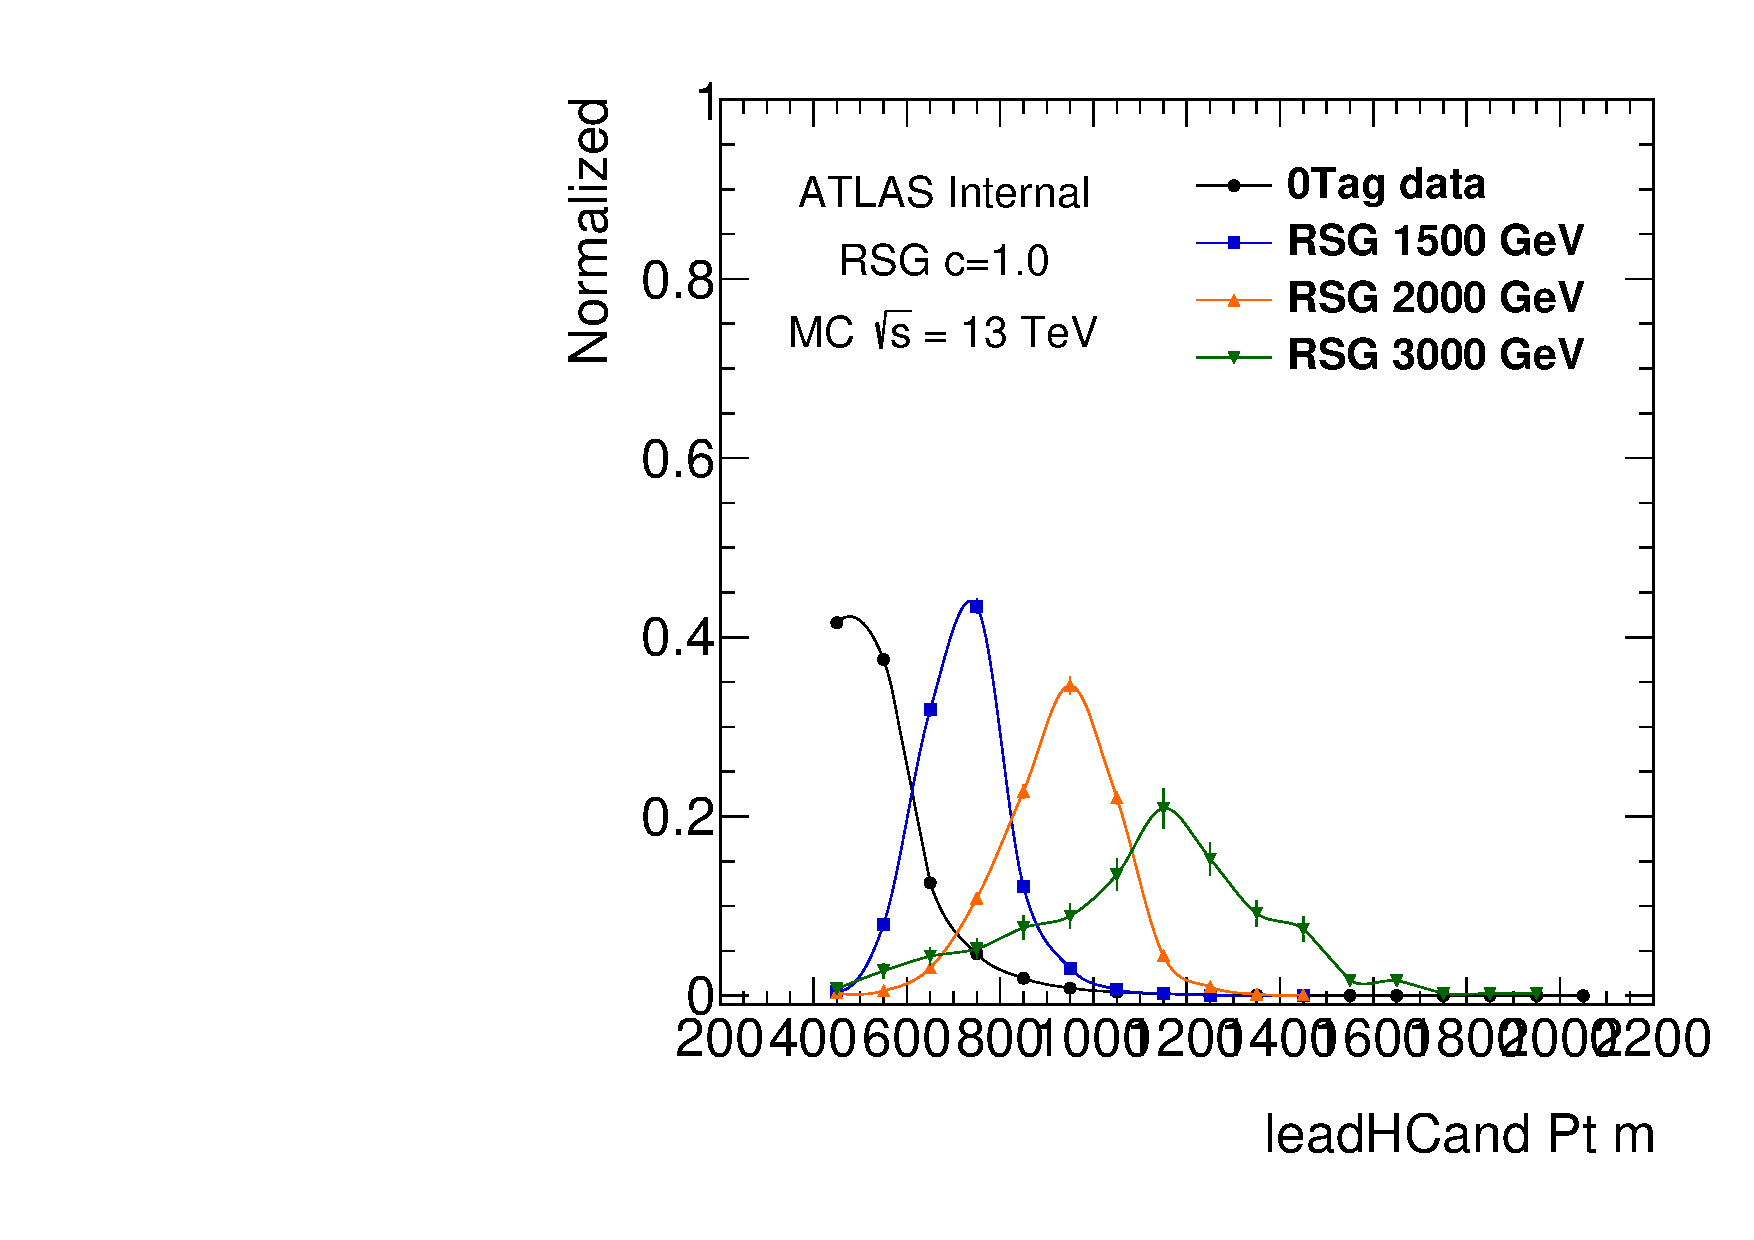
\includegraphics[width=0.32\textwidth,angle=-90]{figures/boosted/Truth/Moriond_comp_0_FourTag_Signal_leadHCand_Pt_m.pdf}
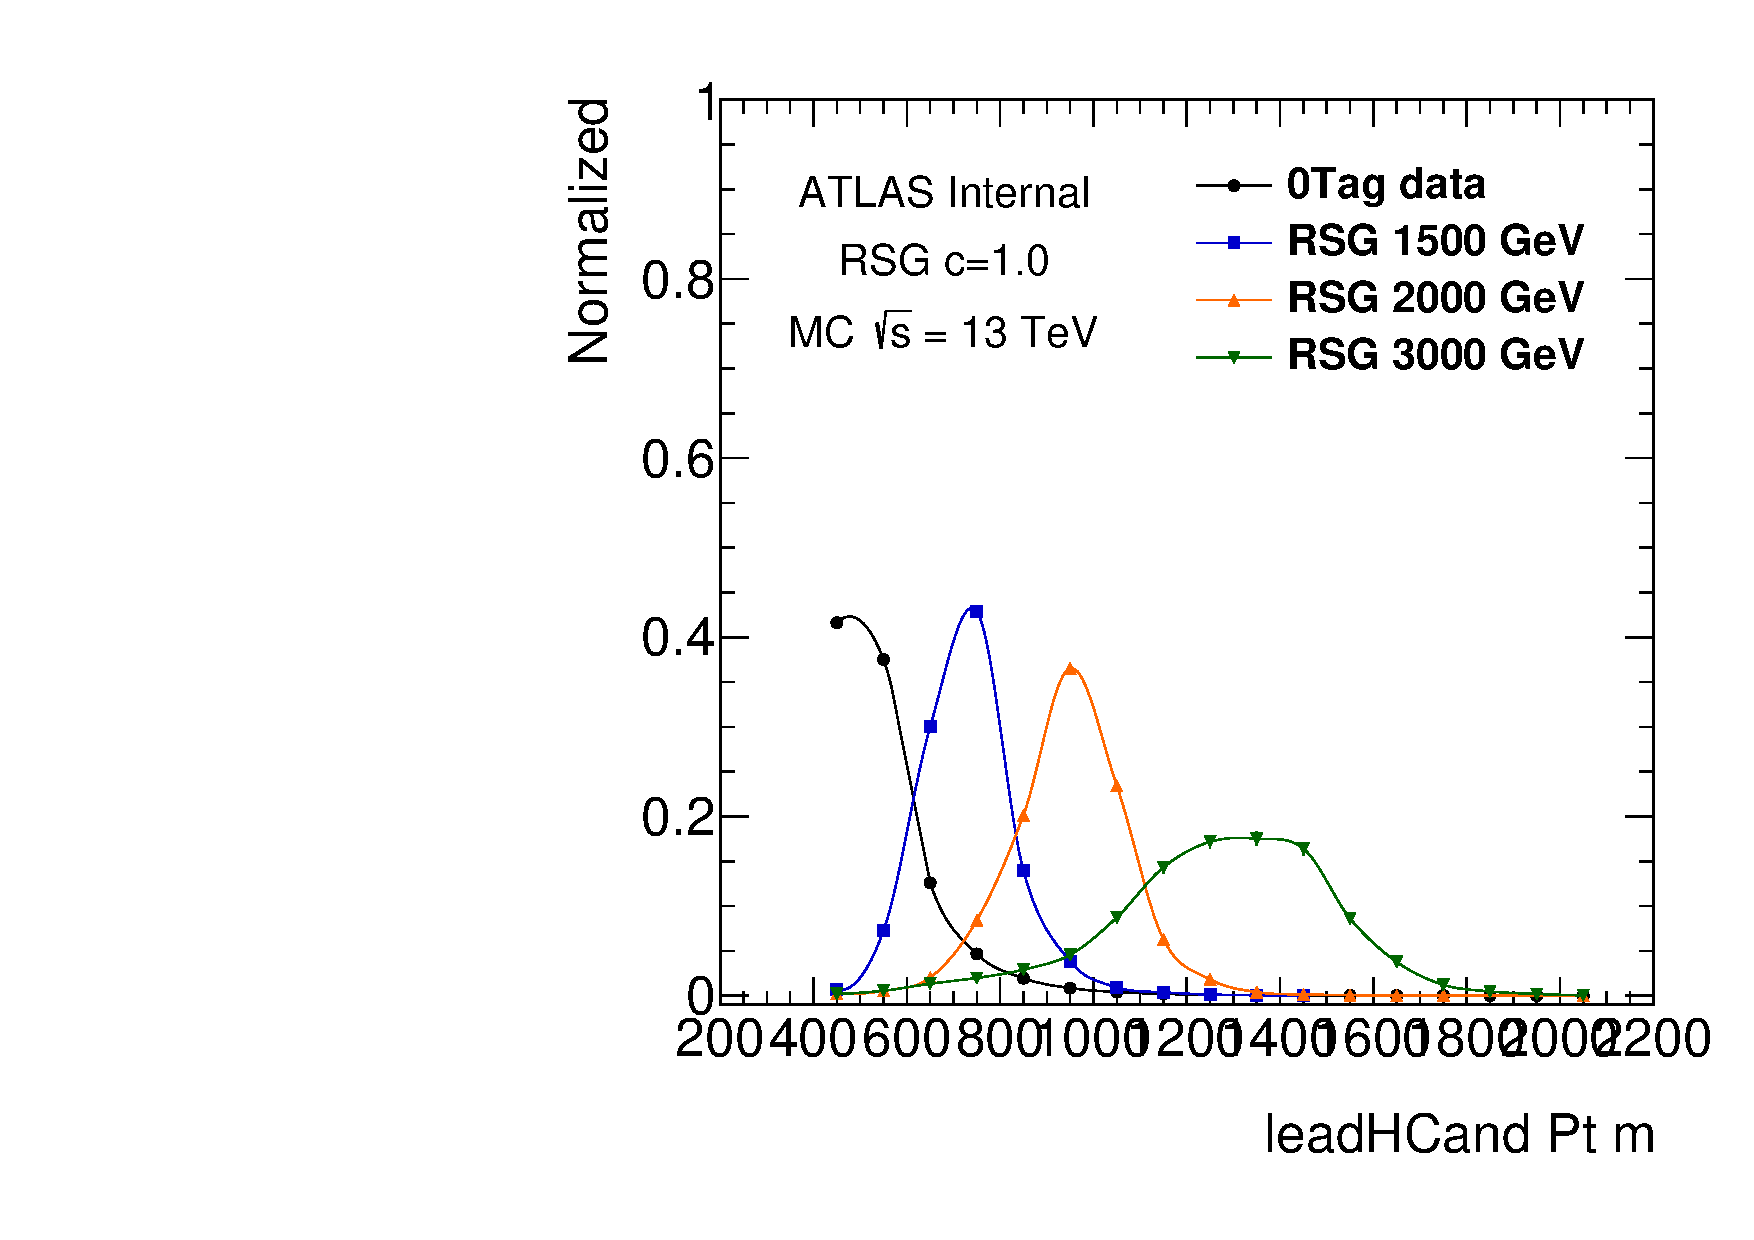
\includegraphics[width=0.32\textwidth,angle=-90]{figures/boosted/Truth/Moriond_comp_0_ThreeTag_Signal_leadHCand_Pt_m.pdf}
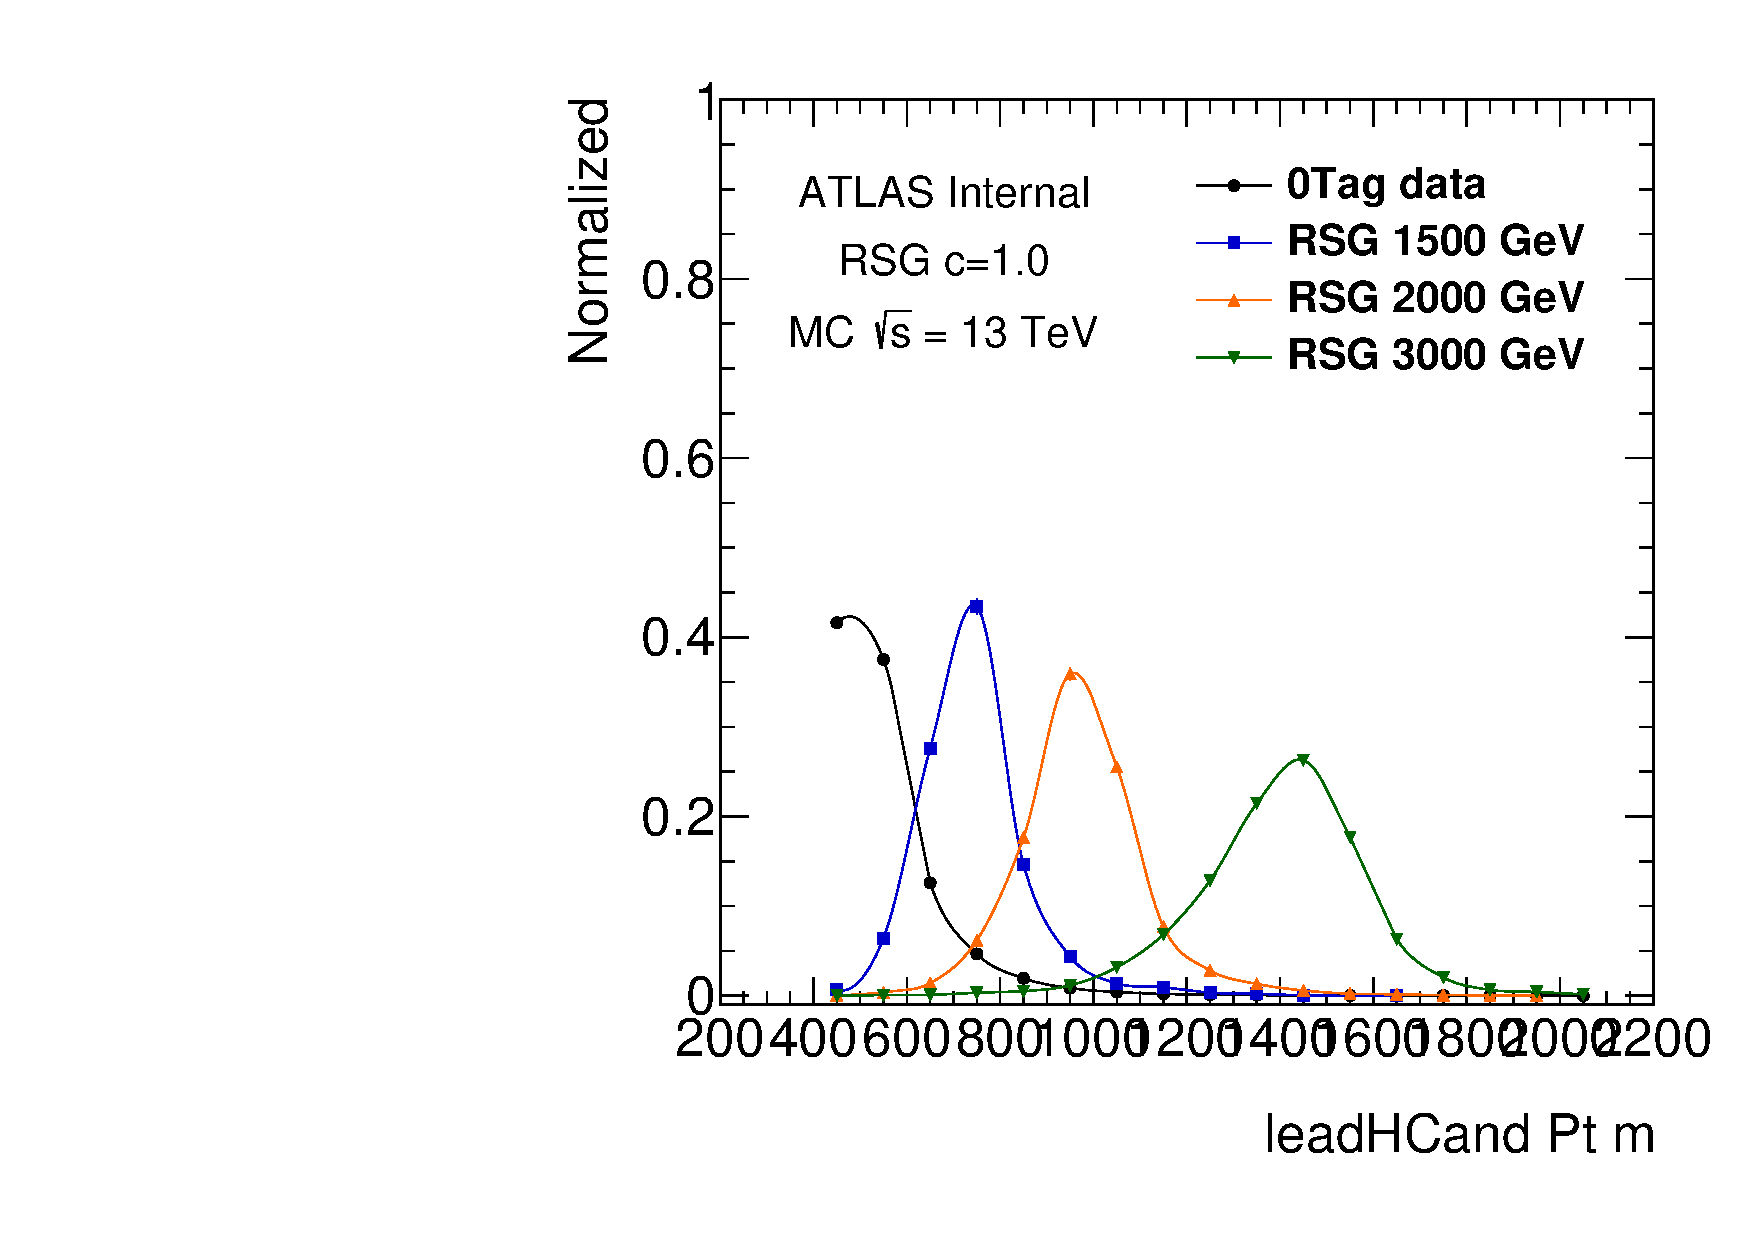
\includegraphics[width=0.32\textwidth,angle=-90]{figures/boosted/Truth/Moriond_comp_0_TwoTag_split_Signal_leadHCand_Pt_m.pdf}\\
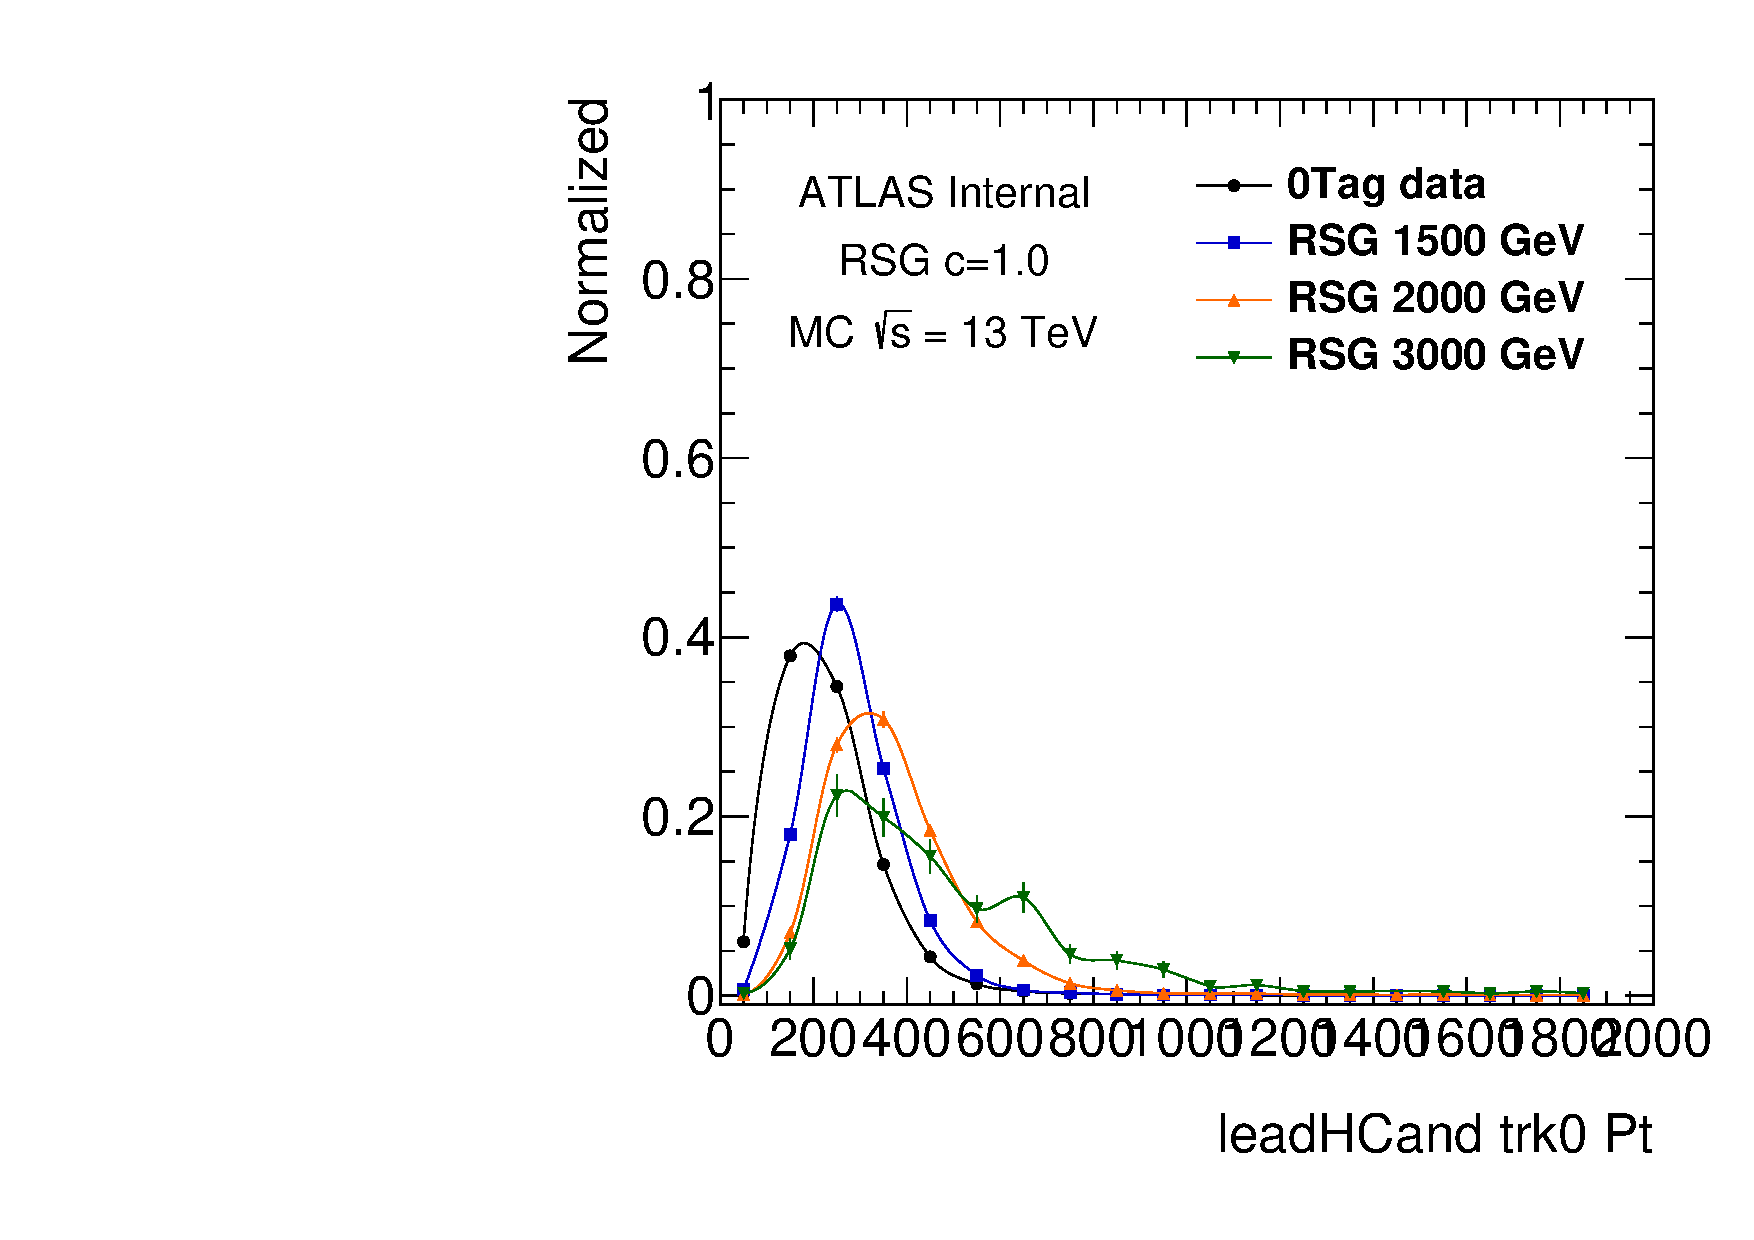
\includegraphics[width=0.32\textwidth,angle=-90]{figures/boosted/Truth/Moriond_comp_0_FourTag_Signal_leadHCand_trk0_Pt.pdf}
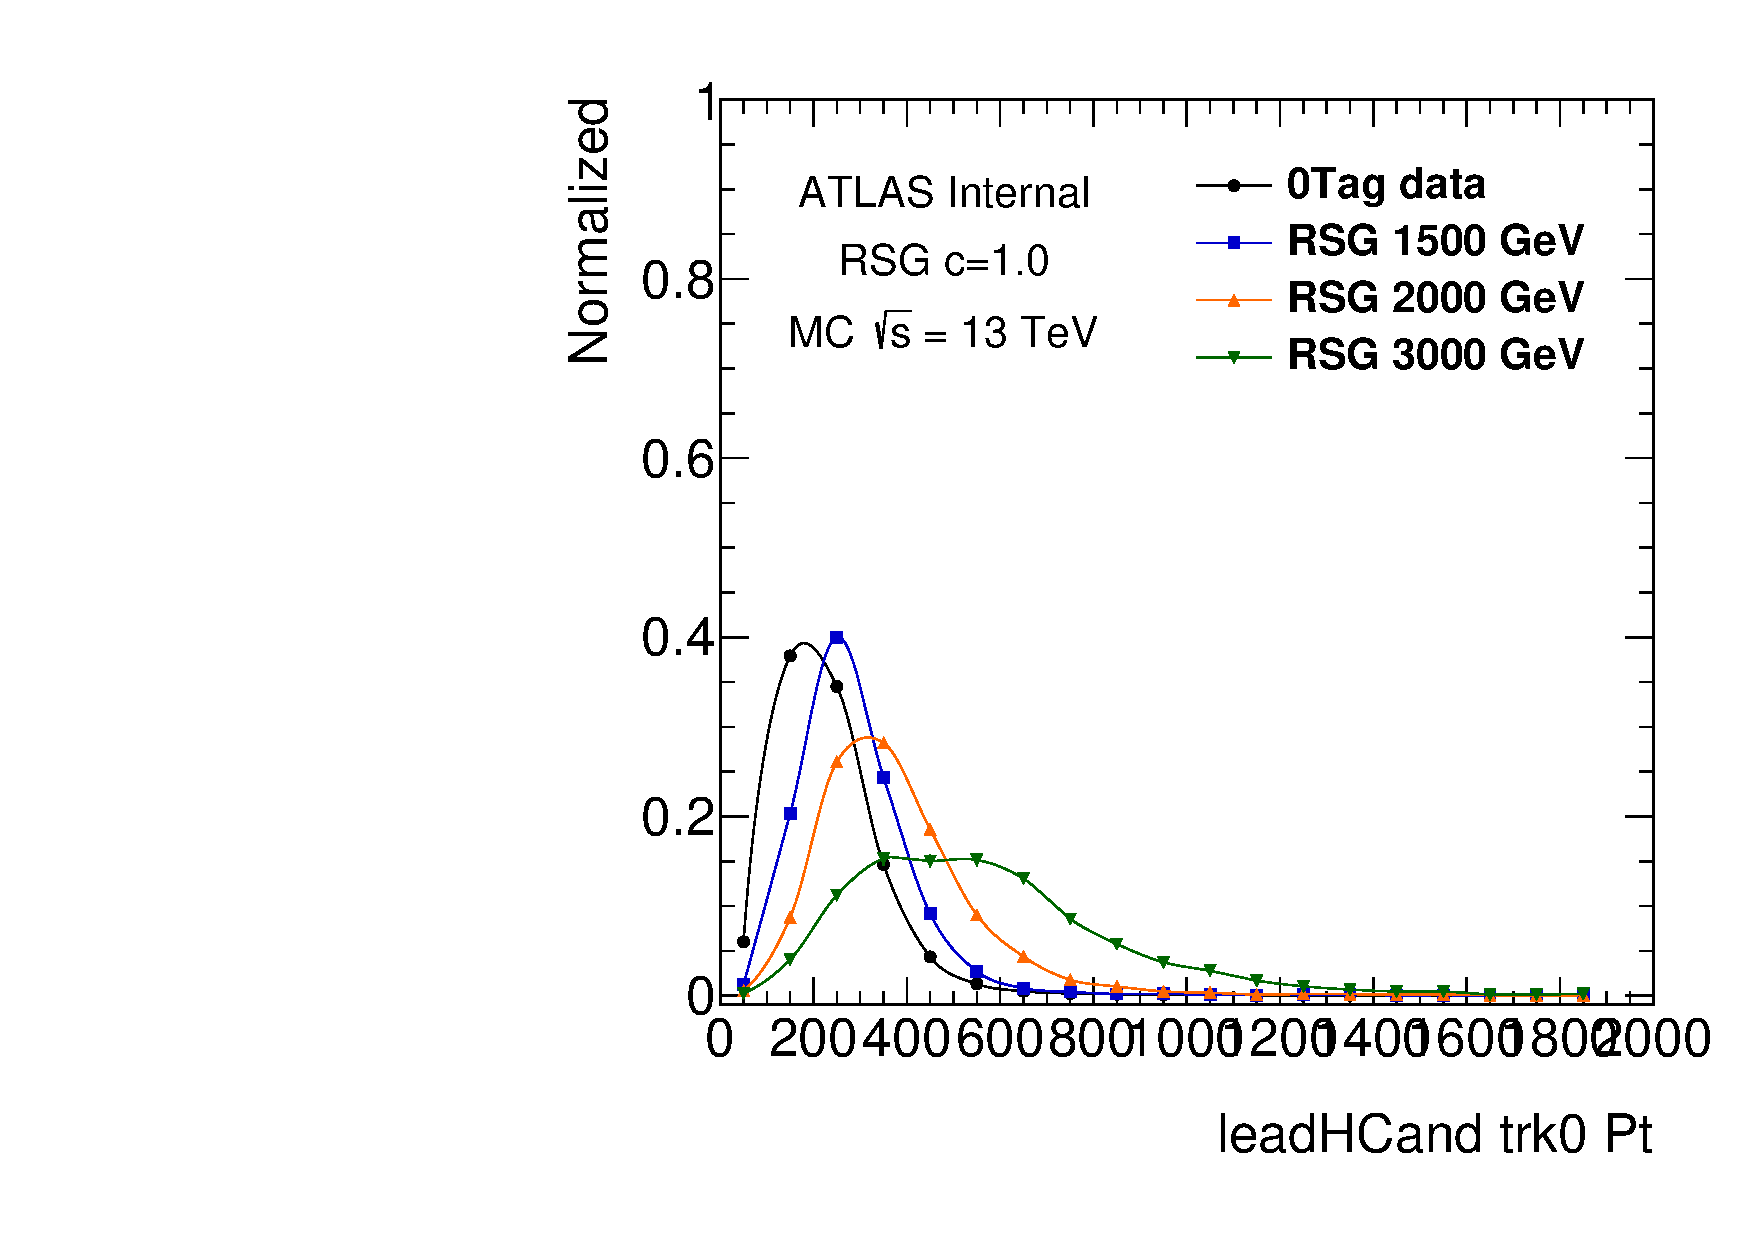
\includegraphics[width=0.32\textwidth,angle=-90]{figures/boosted/Truth/Moriond_comp_0_ThreeTag_Signal_leadHCand_trk0_Pt.pdf}
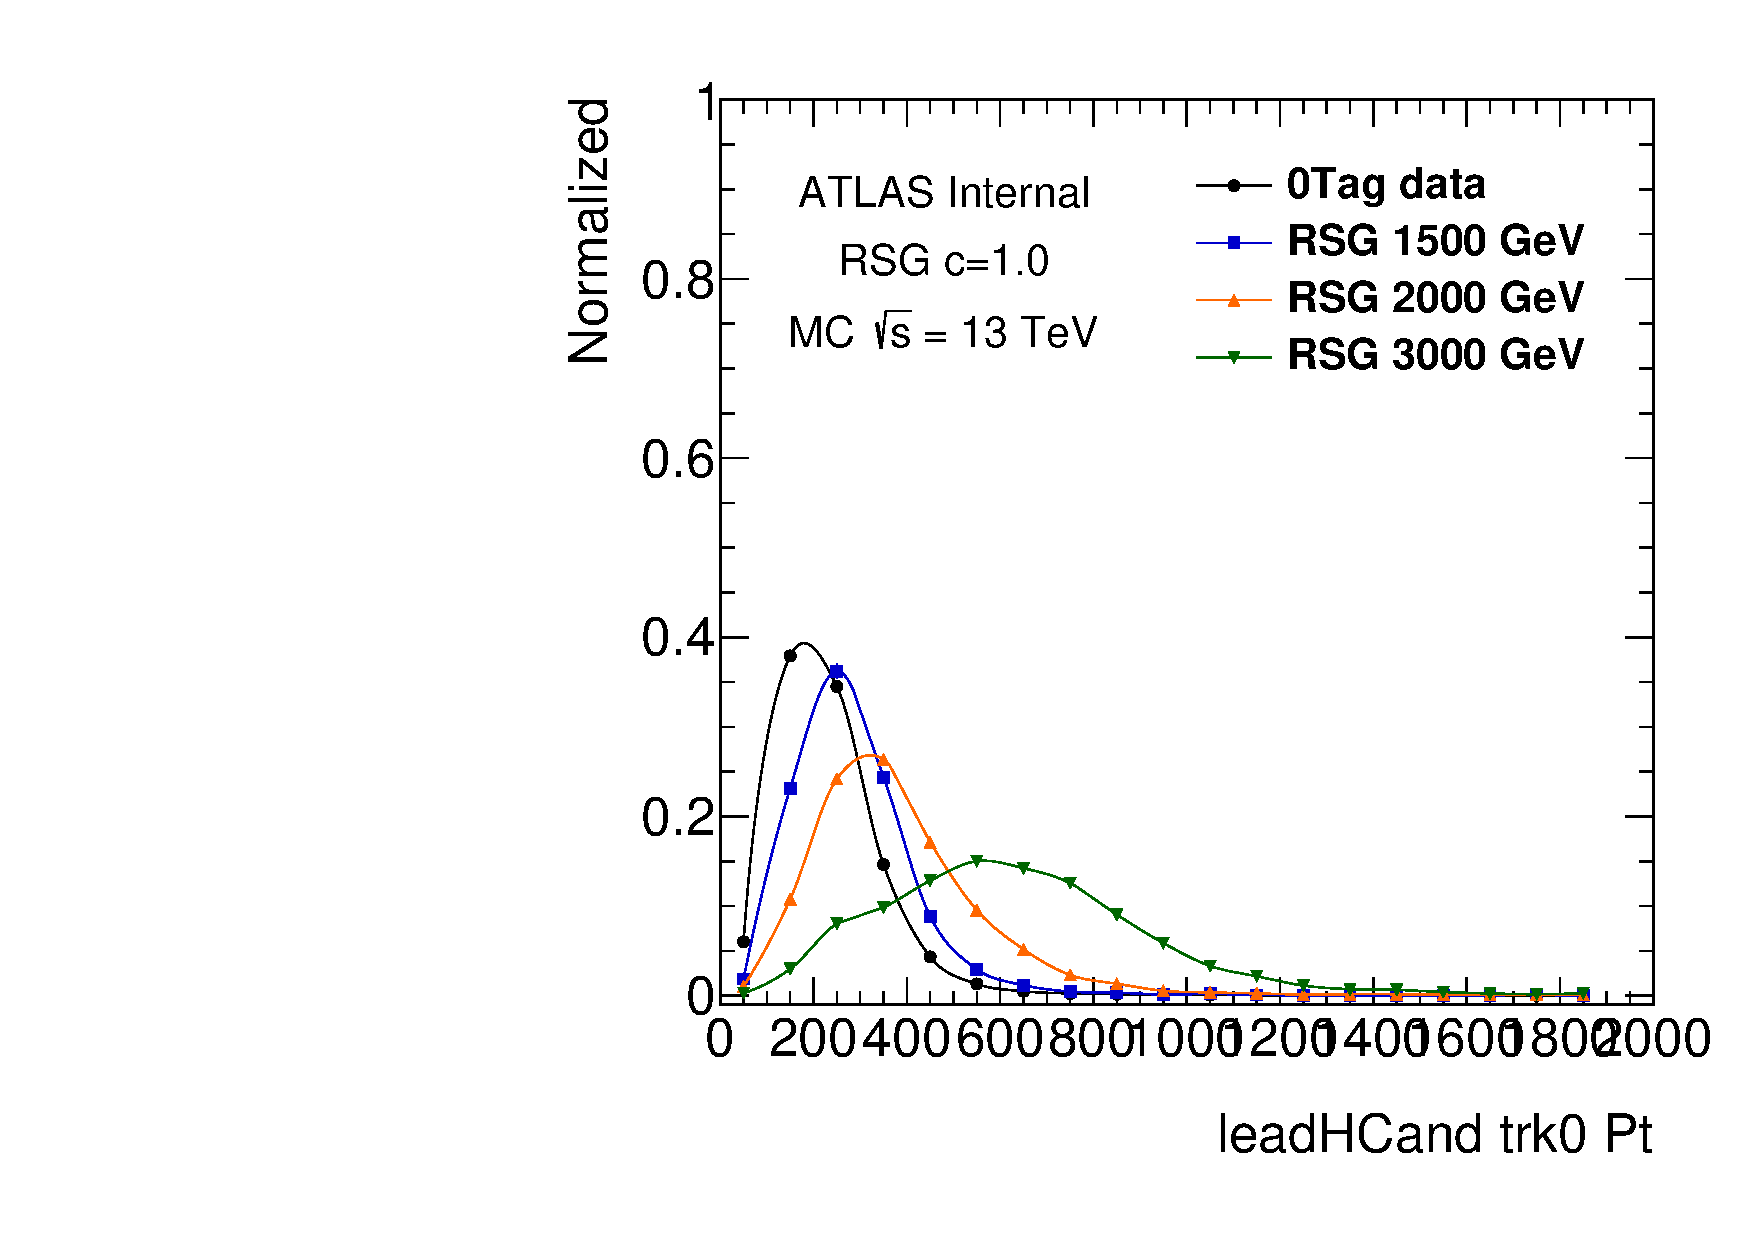
\includegraphics[width=0.32\textwidth,angle=-90]{figures/boosted/Truth/Moriond_comp_0_TwoTag_split_Signal_leadHCand_trk0_Pt.pdf}\\
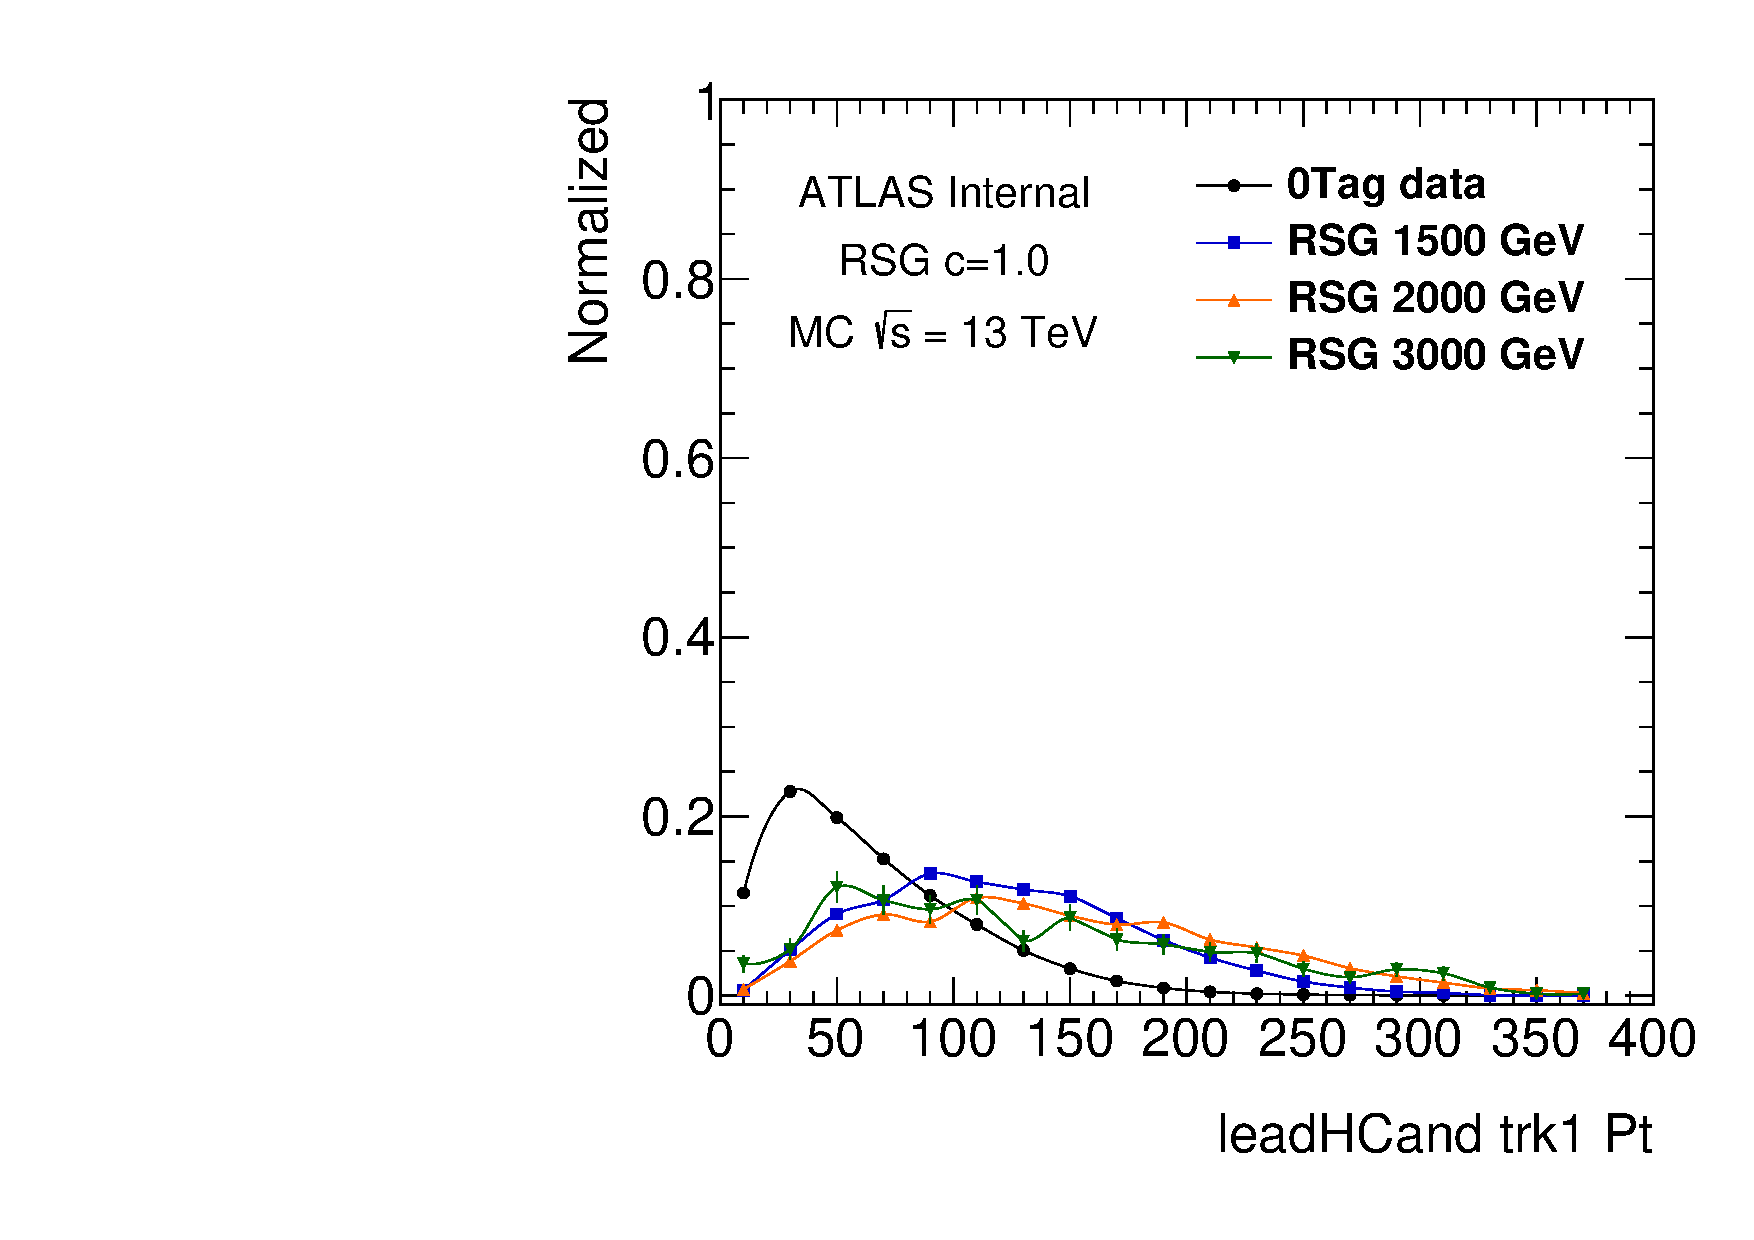
\includegraphics[width=0.32\textwidth,angle=-90]{figures/boosted/Truth/Moriond_comp_0_FourTag_Signal_leadHCand_trk1_Pt.pdf}
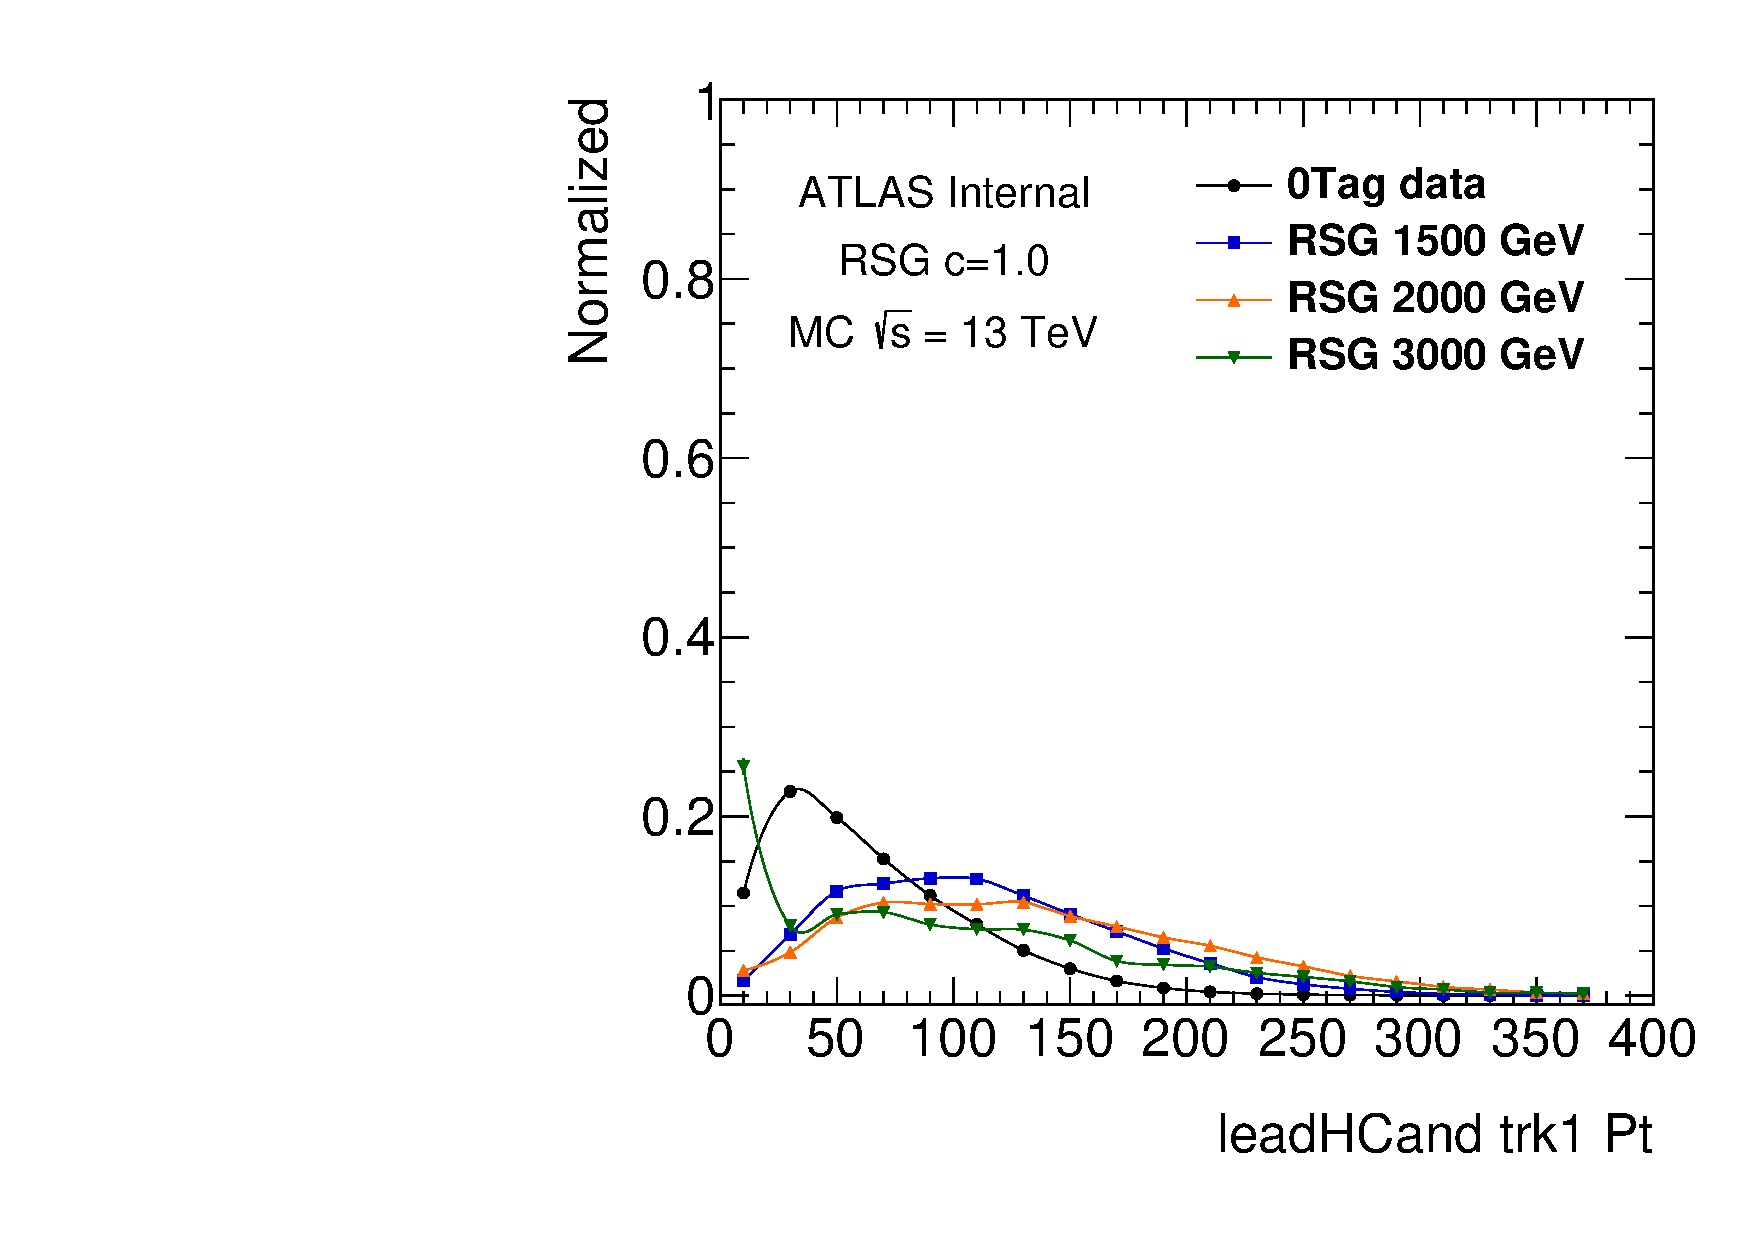
\includegraphics[width=0.32\textwidth,angle=-90]{figures/boosted/Truth/Moriond_comp_0_ThreeTag_Signal_leadHCand_trk1_Pt.pdf}
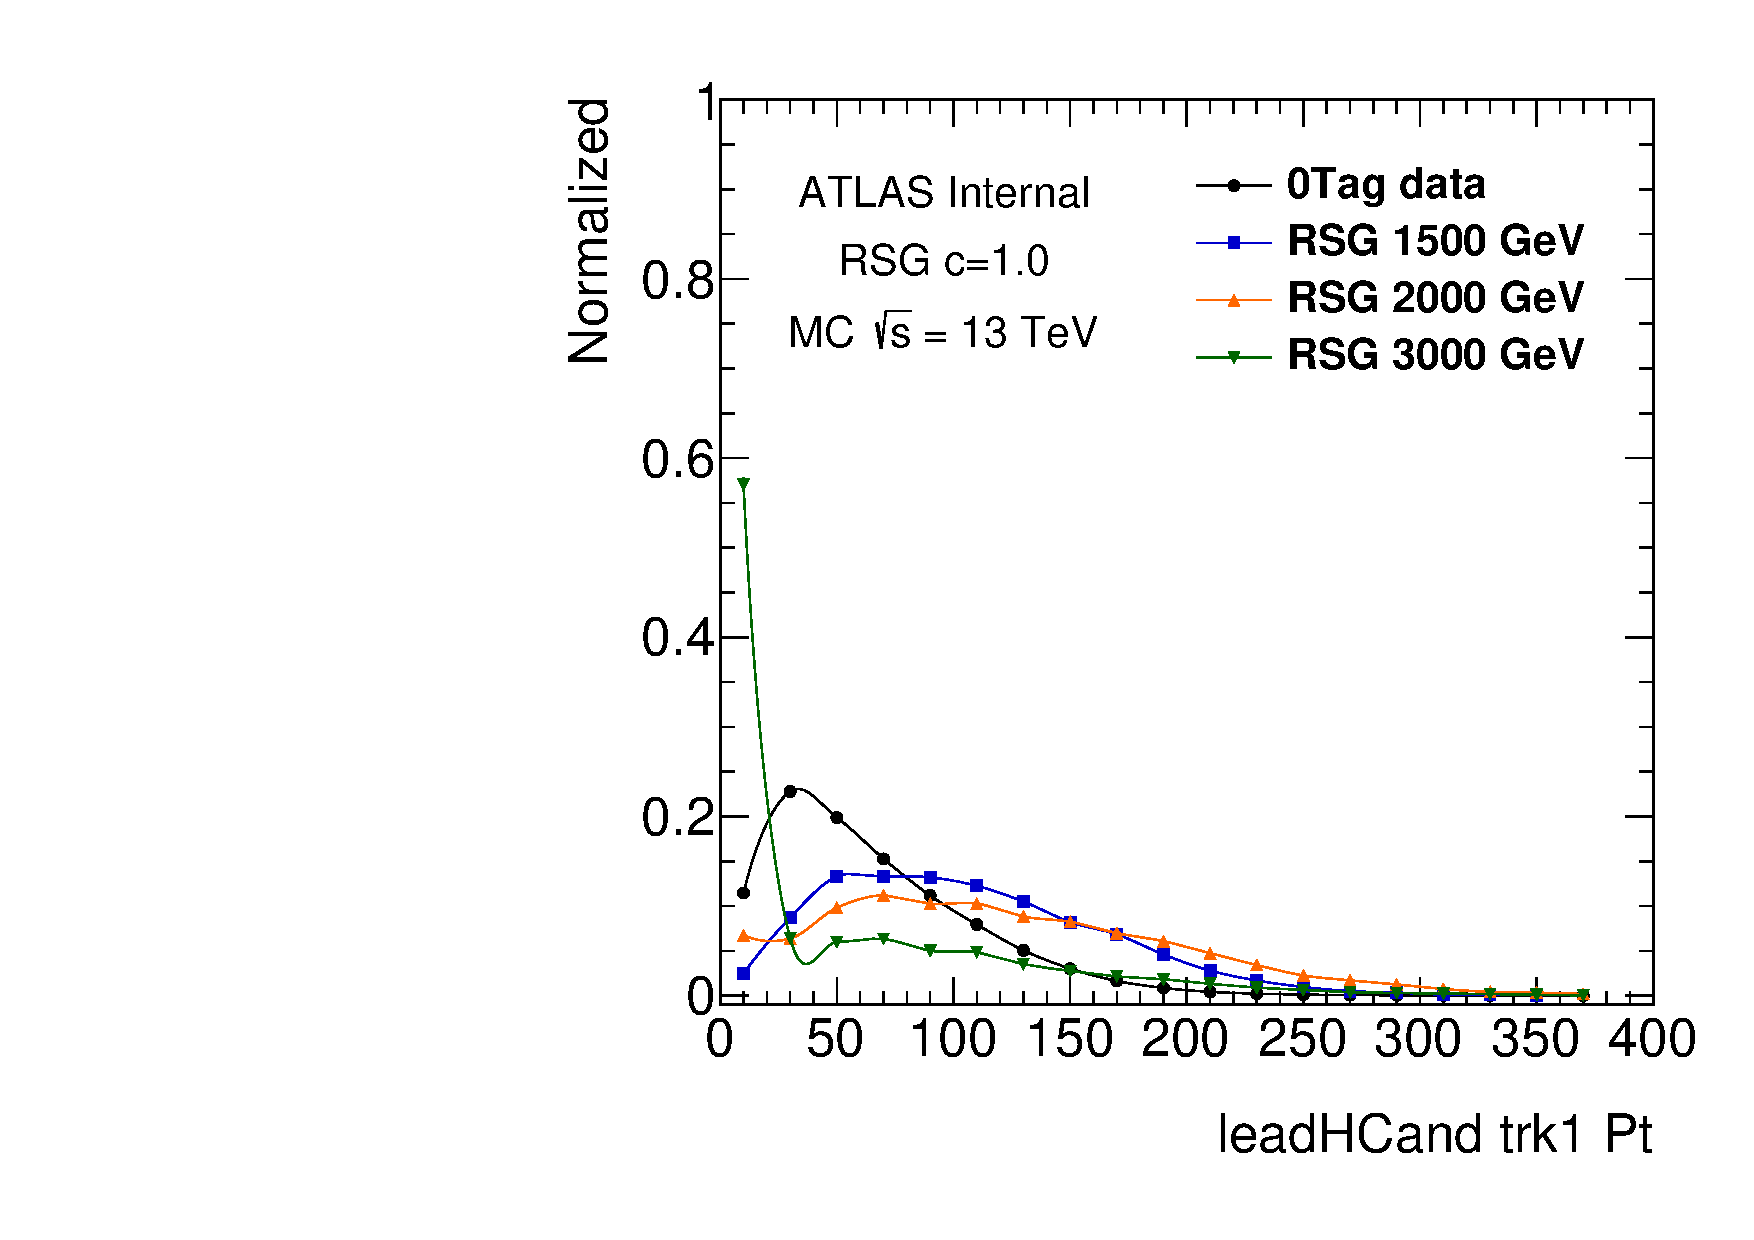
\includegraphics[width=0.32\textwidth,angle=-90]{figures/boosted/Truth/Moriond_comp_0_TwoTag_split_Signal_leadHCand_trk1_Pt.pdf}\\
\caption{For RSG $c=1.0$ samples, the leading higgs candidate's $p_T$, mass, leading track jet $p_T$ and subleading trackjet $p_T$. The left column is $4b$, the middle column is $3b$, and the right column is $2bs$.}
\label{fig:app-signal-leadHCand}
\end{center}
\end{figure*}



\begin{figure*}[htbp!]
\begin{center}
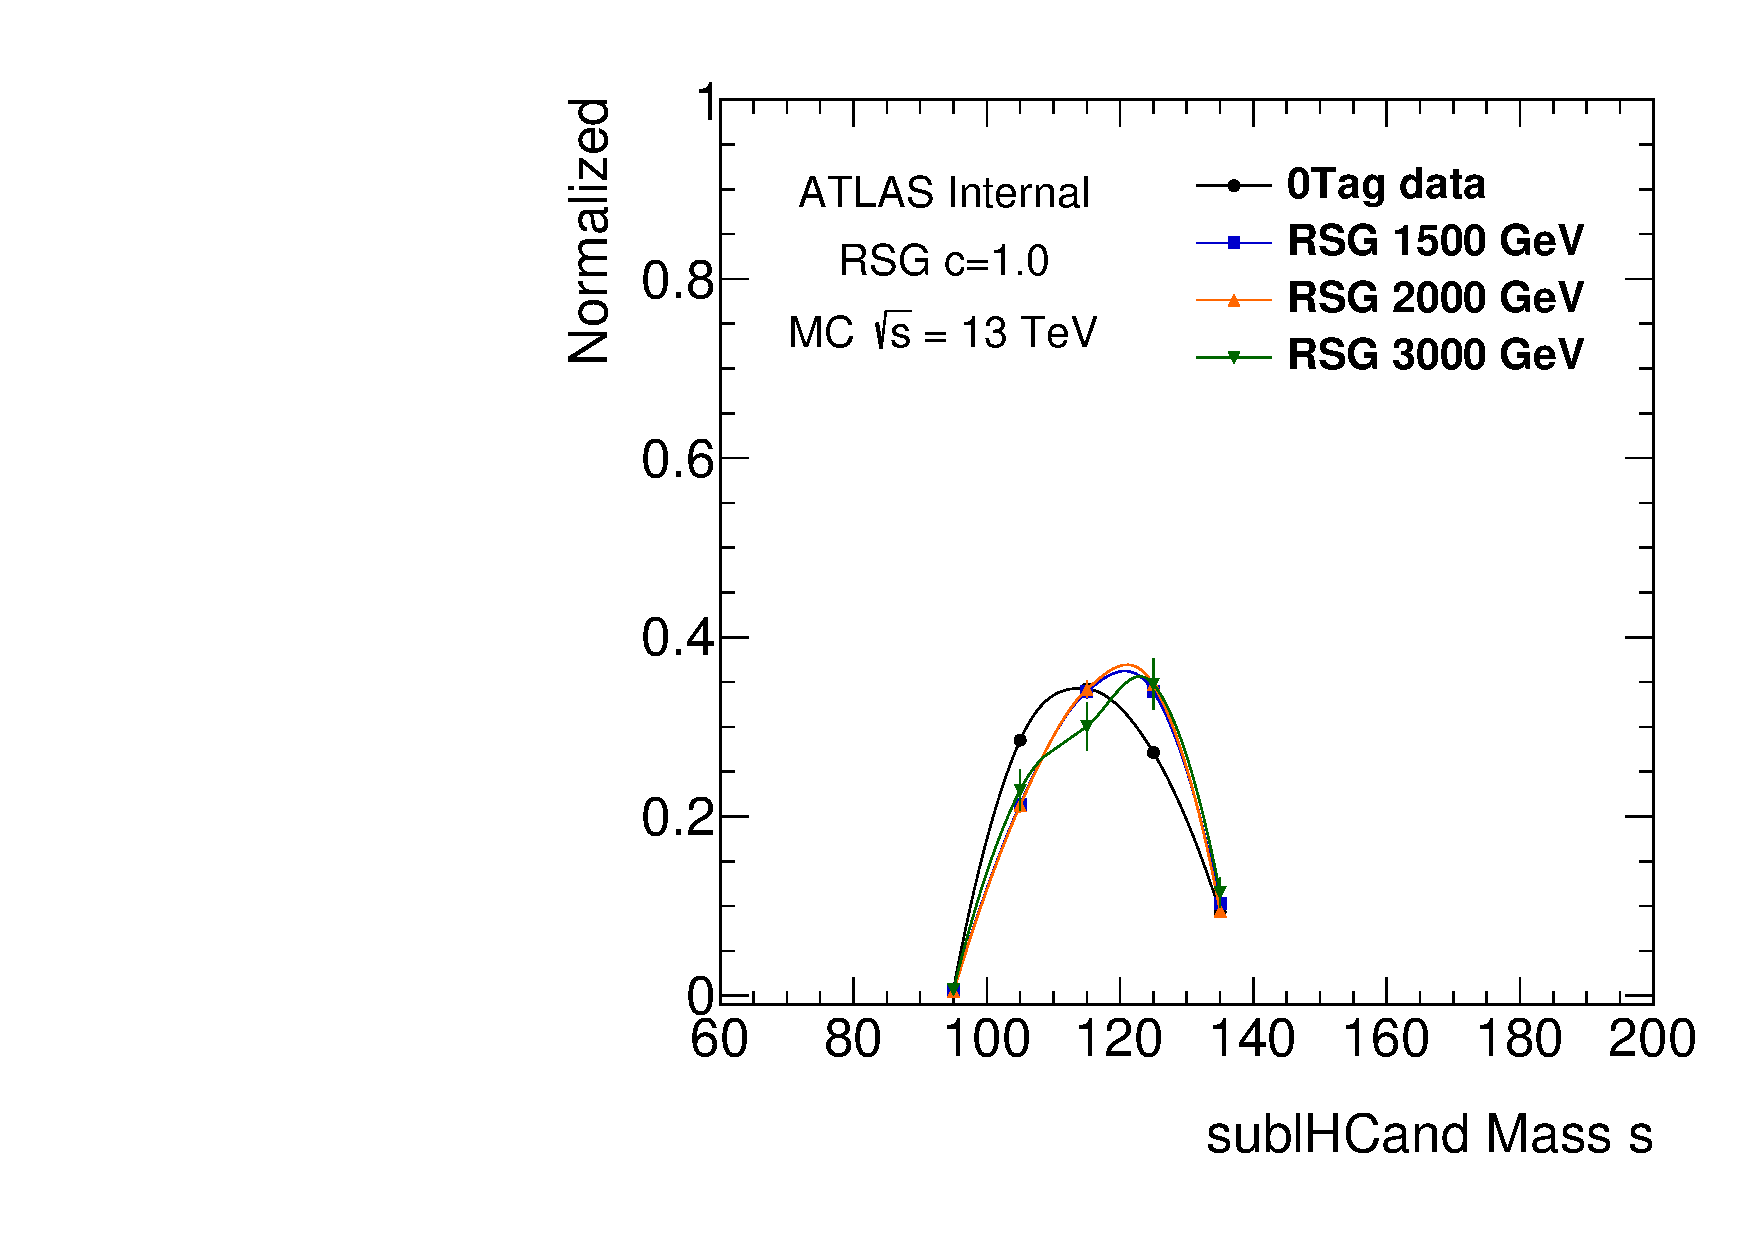
\includegraphics[width=0.32\textwidth,angle=-90]{figures/boosted/Truth/Moriond_comp_0_FourTag_Signal_sublHCand_Mass_s.pdf}
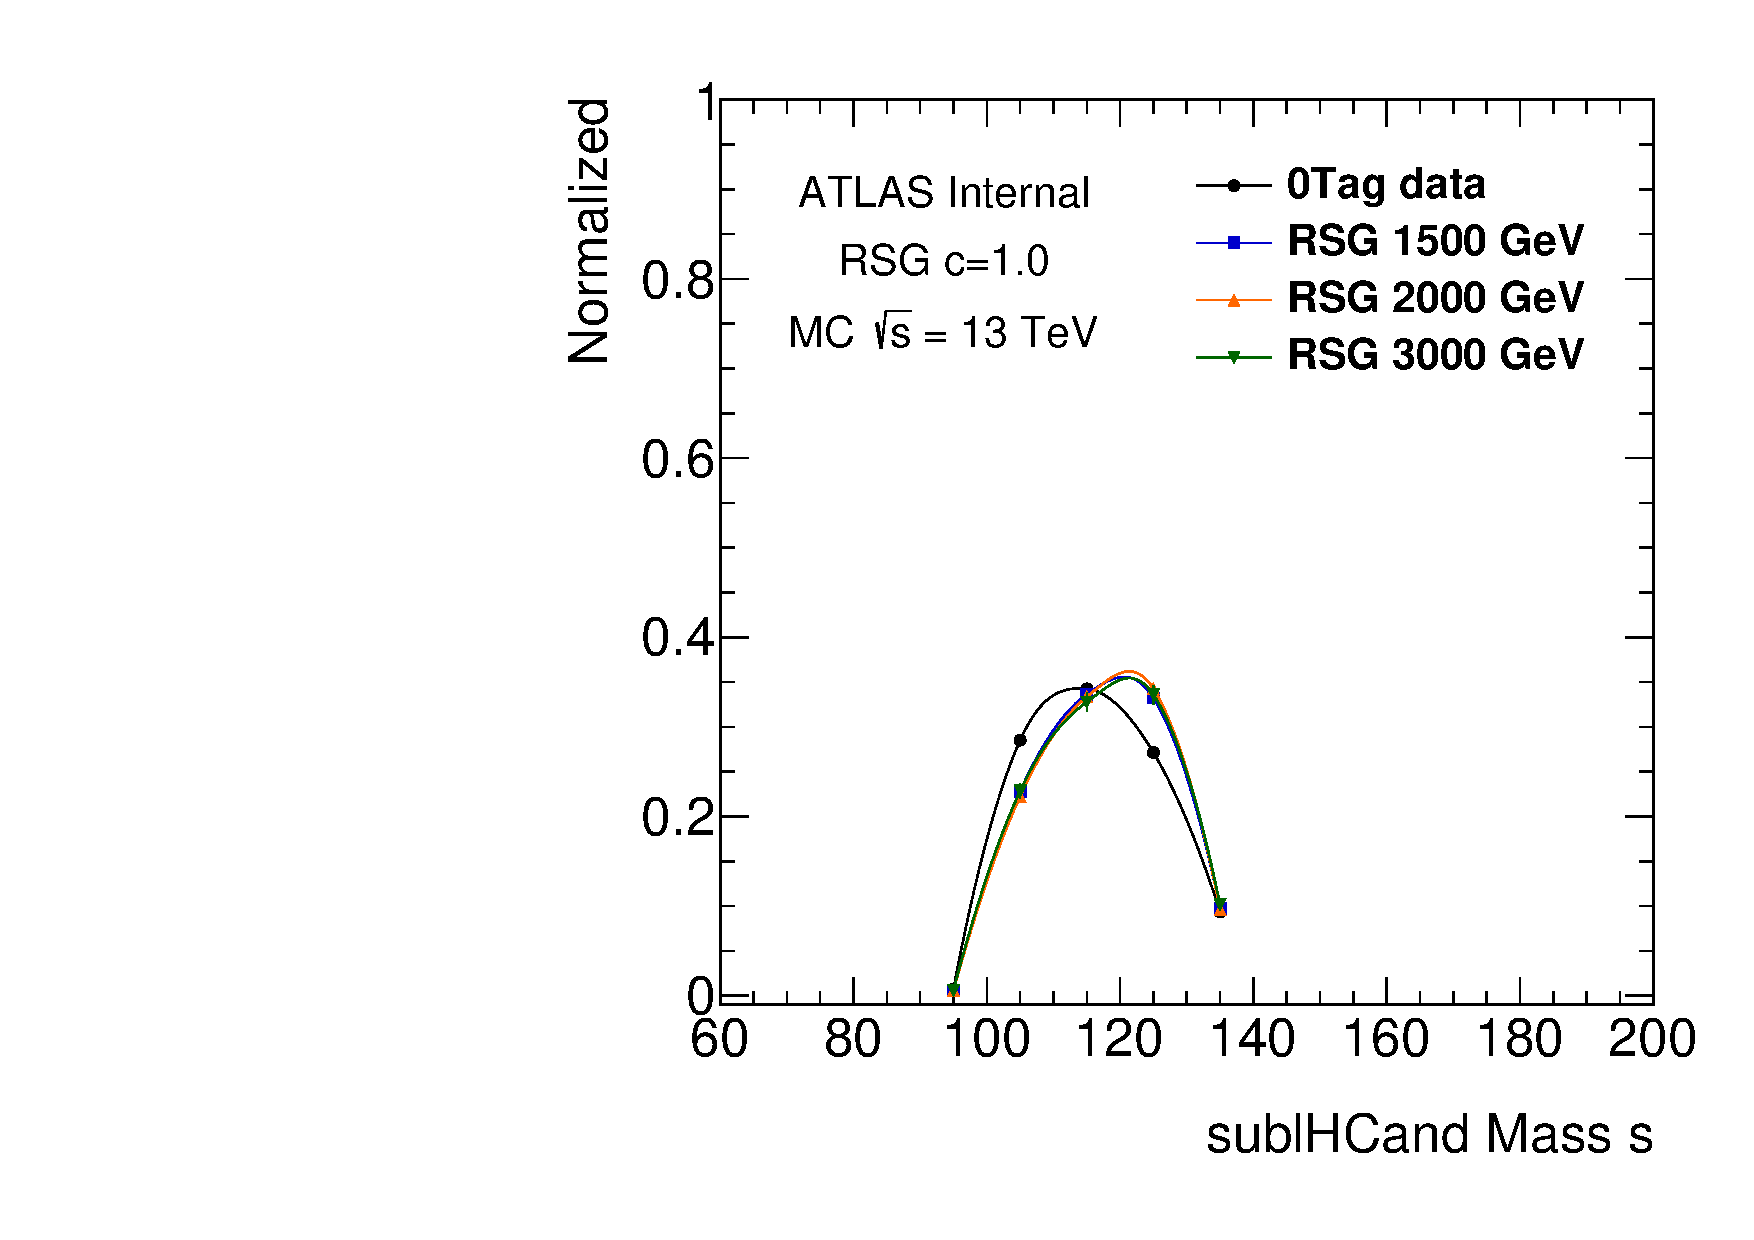
\includegraphics[width=0.32\textwidth,angle=-90]{figures/boosted/Truth/Moriond_comp_0_ThreeTag_Signal_sublHCand_Mass_s.pdf}
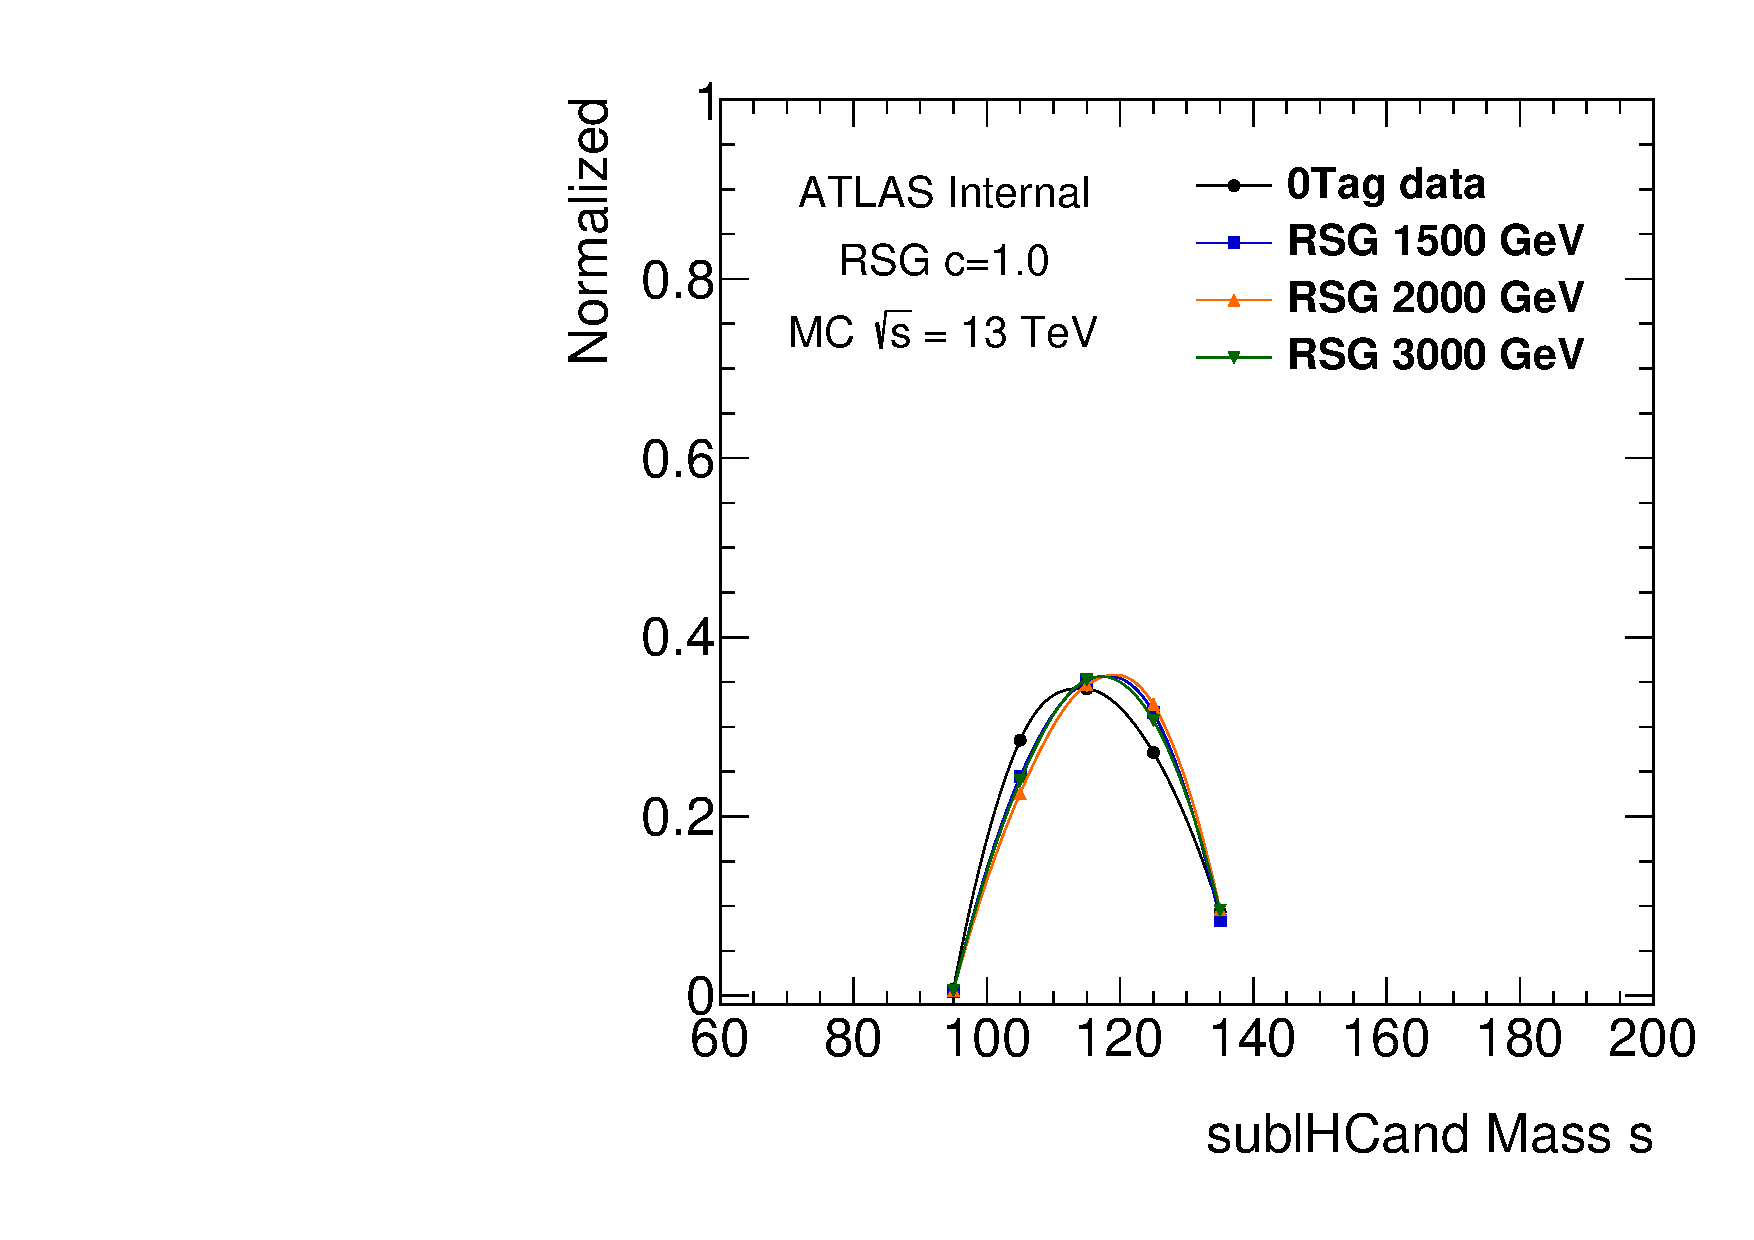
\includegraphics[width=0.32\textwidth,angle=-90]{figures/boosted/Truth/Moriond_comp_0_TwoTag_split_Signal_sublHCand_Mass_s.pdf}\\
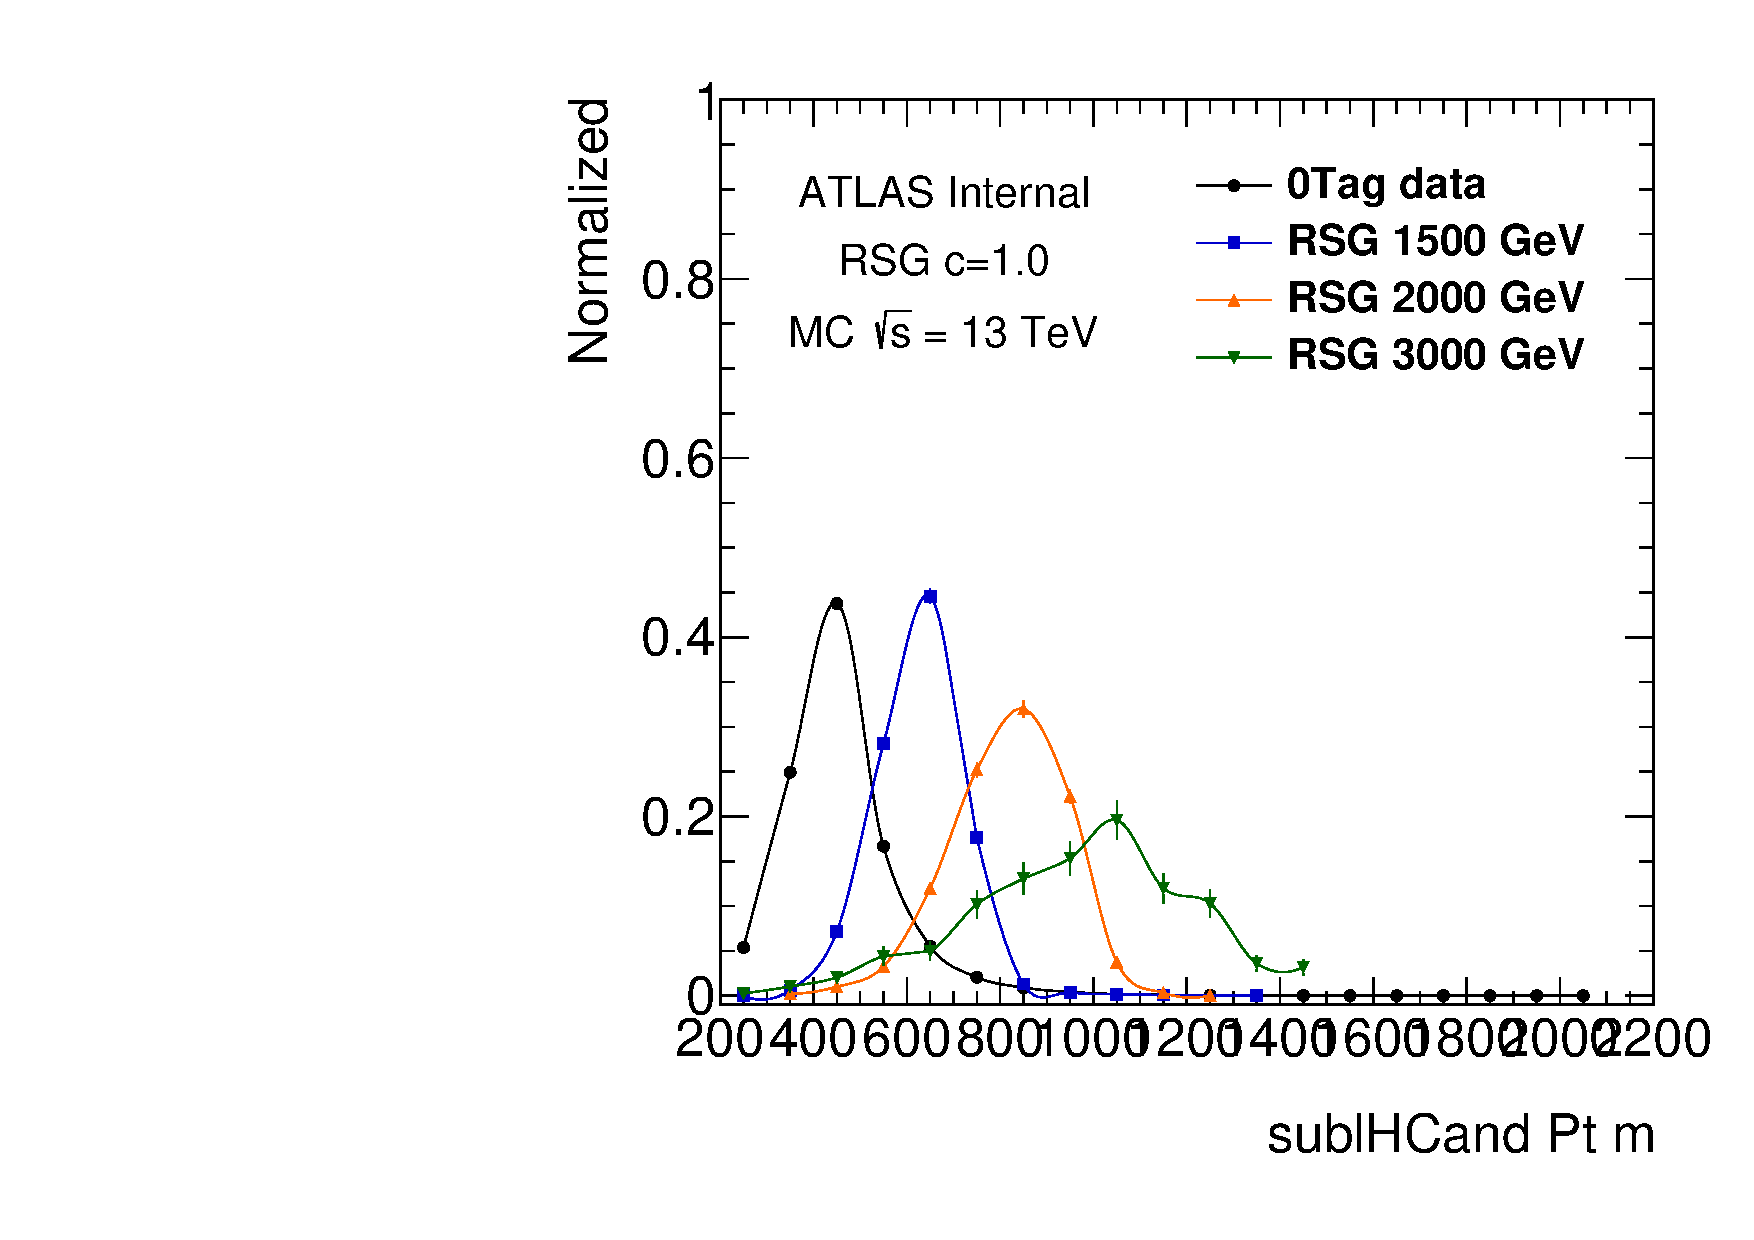
\includegraphics[width=0.32\textwidth,angle=-90]{figures/boosted/Truth/Moriond_comp_0_FourTag_Signal_sublHCand_Pt_m.pdf}
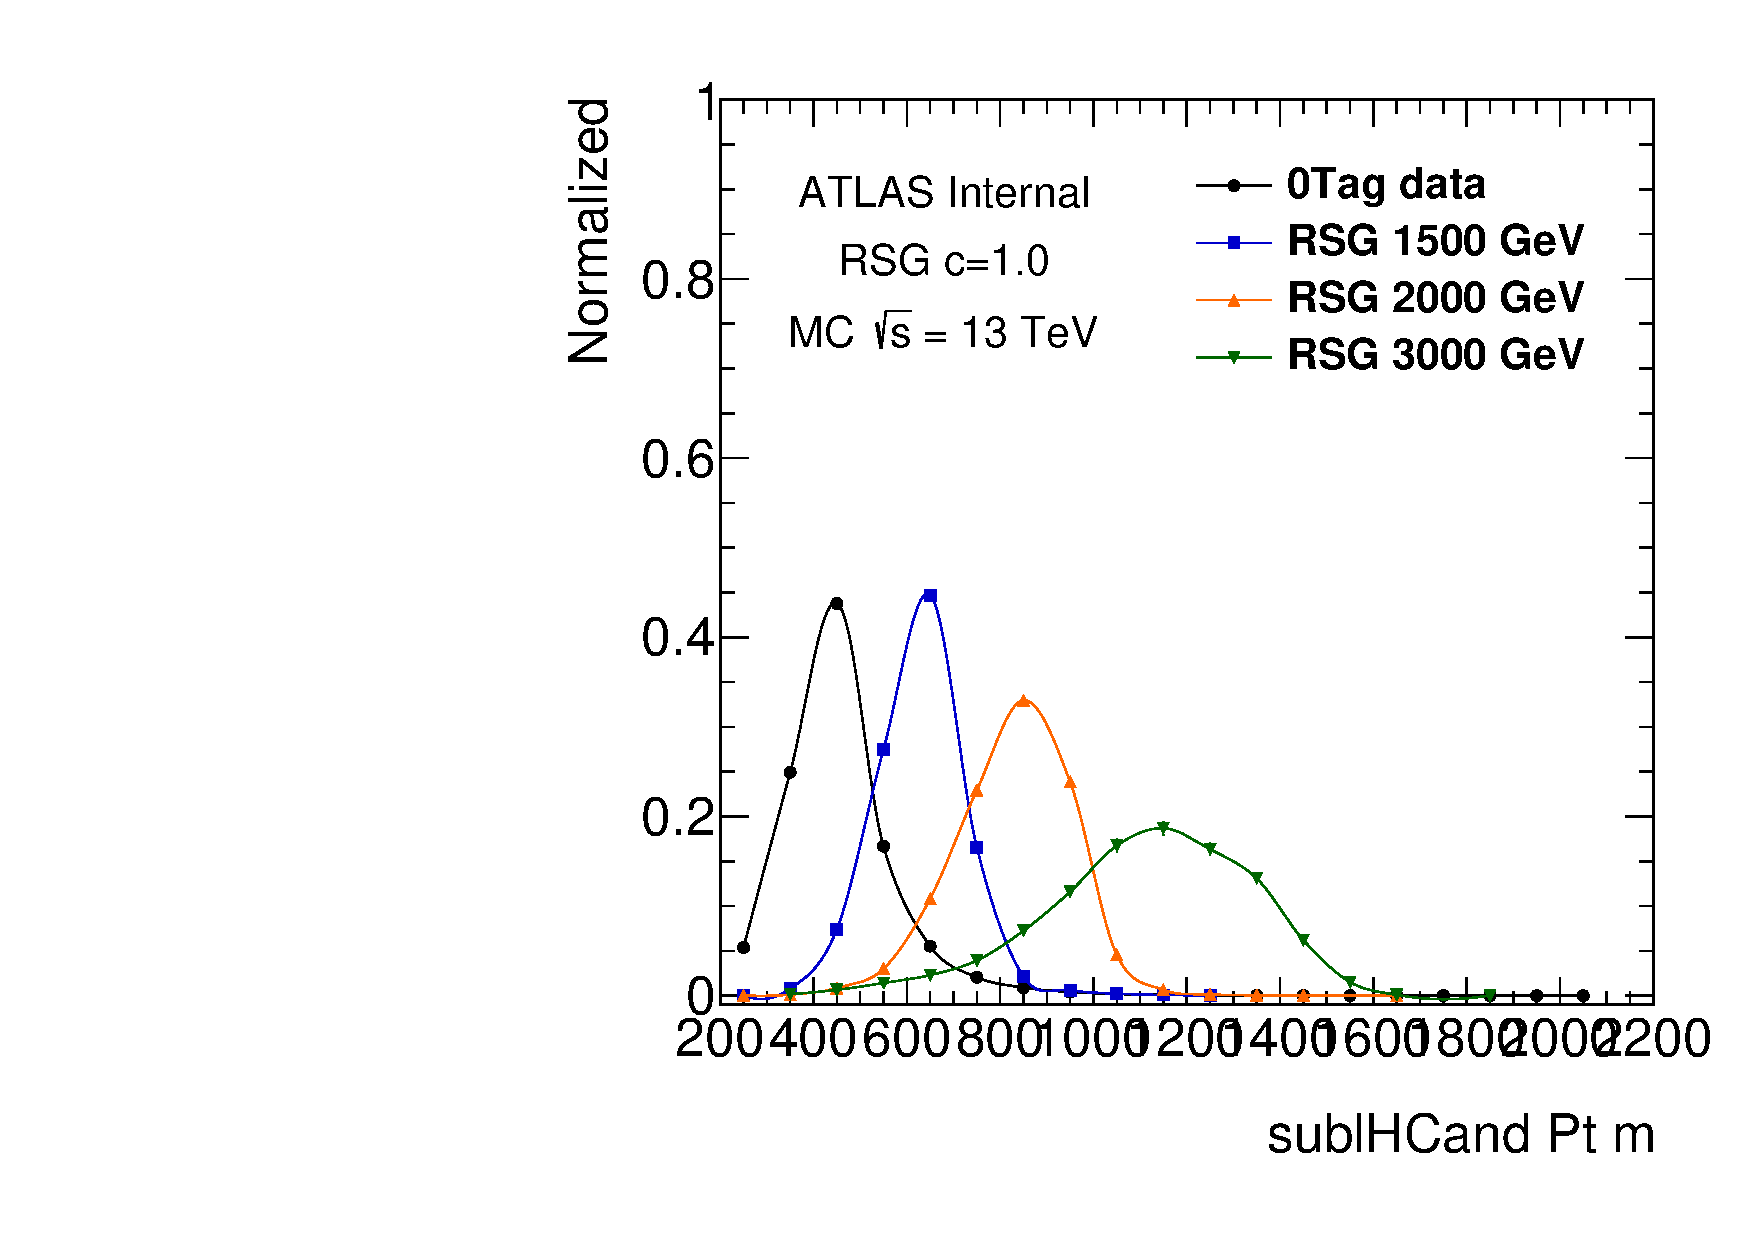
\includegraphics[width=0.32\textwidth,angle=-90]{figures/boosted/Truth/Moriond_comp_0_ThreeTag_Signal_sublHCand_Pt_m.pdf}
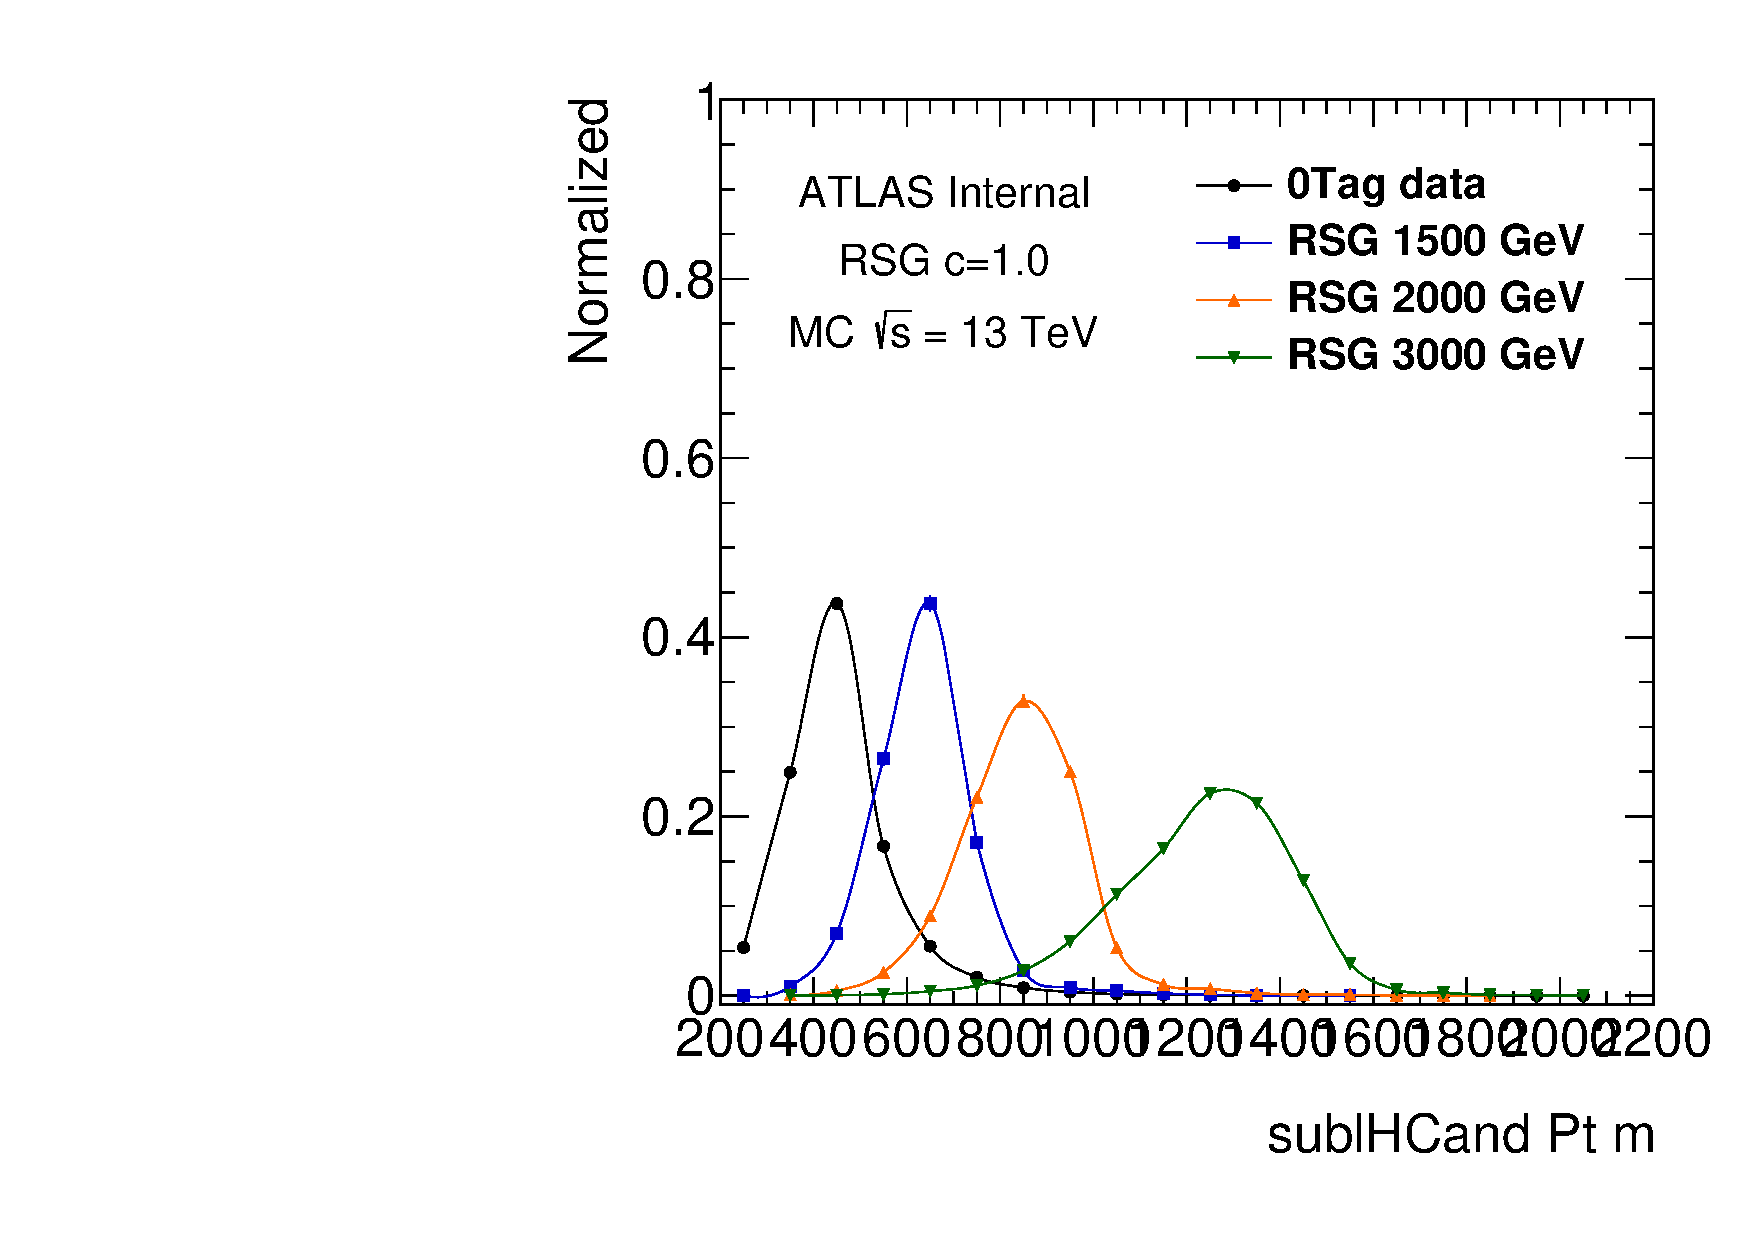
\includegraphics[width=0.32\textwidth,angle=-90]{figures/boosted/Truth/Moriond_comp_0_TwoTag_split_Signal_sublHCand_Pt_m.pdf}\\
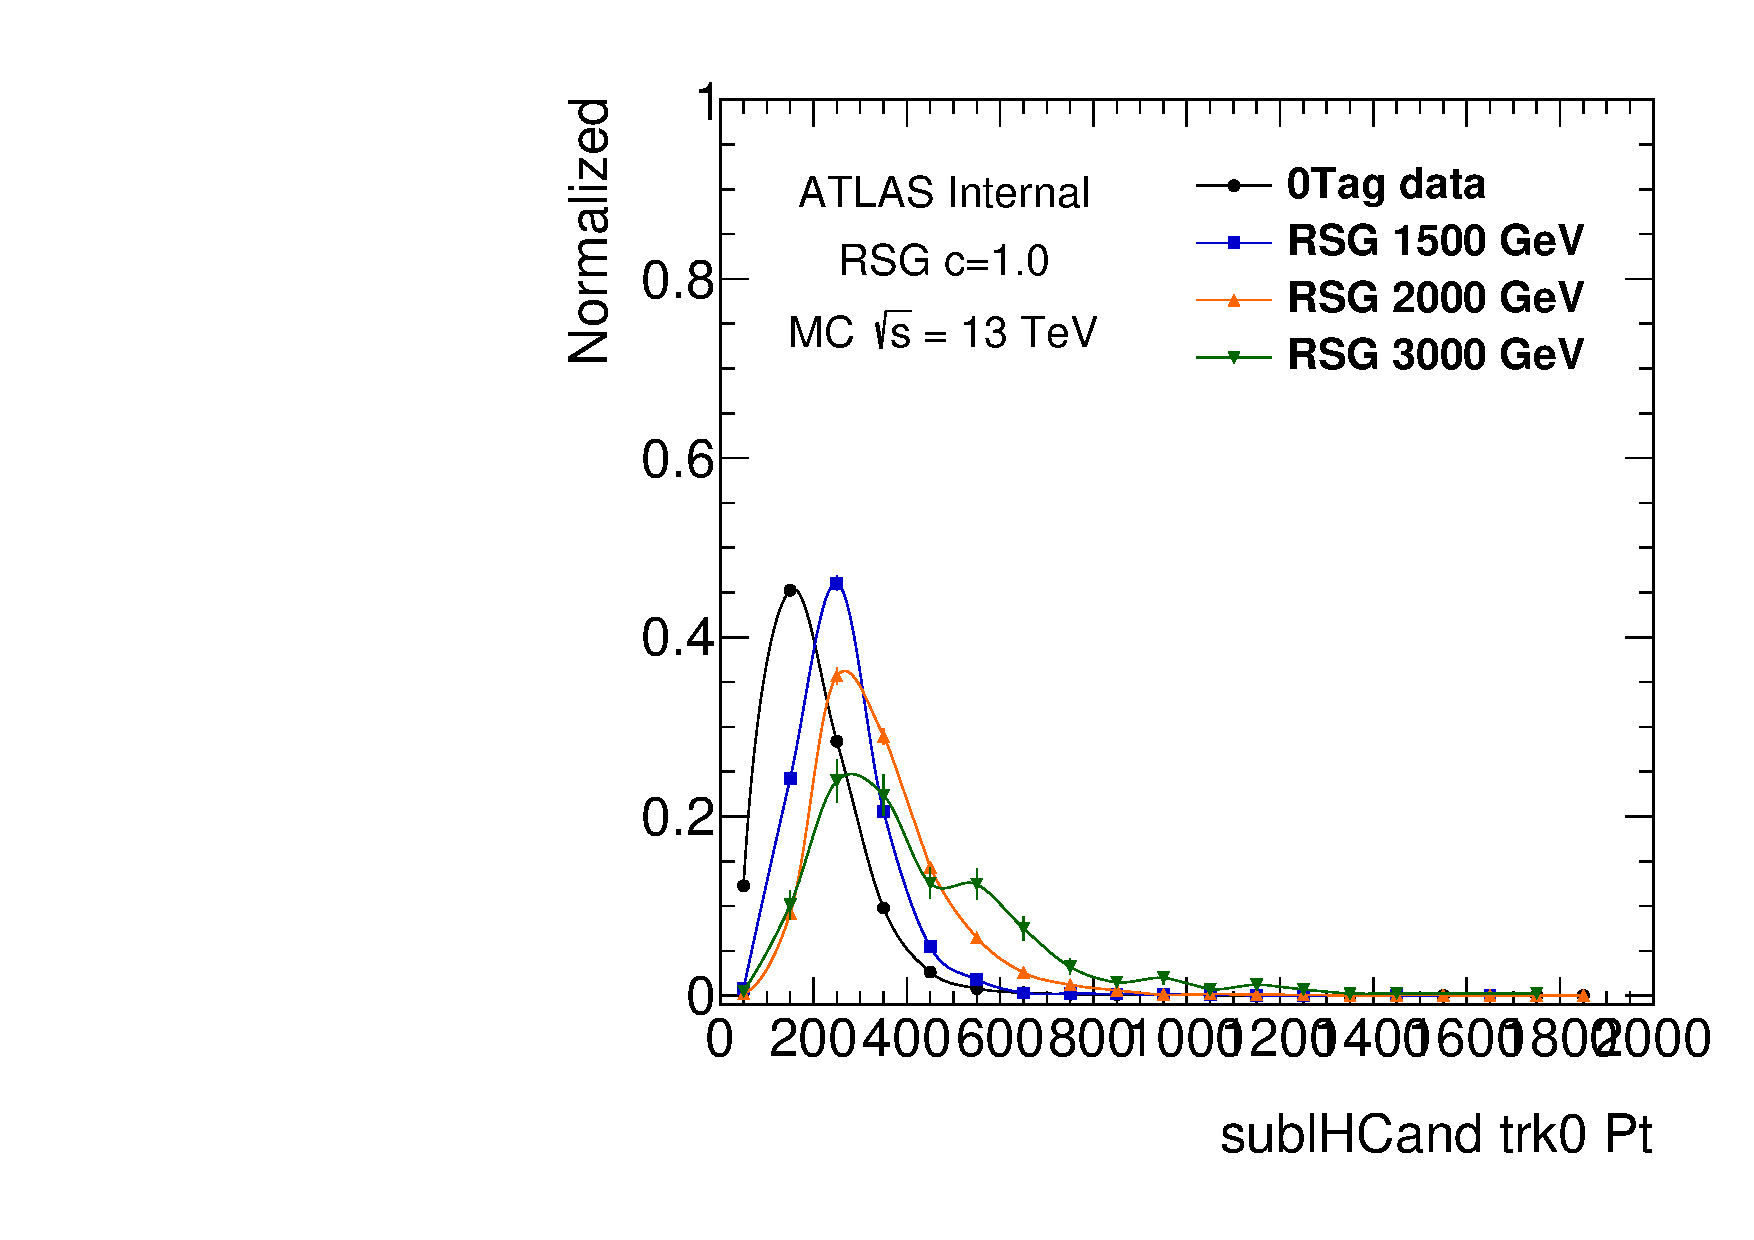
\includegraphics[width=0.32\textwidth,angle=-90]{figures/boosted/Truth/Moriond_comp_0_FourTag_Signal_sublHCand_trk0_Pt.pdf}
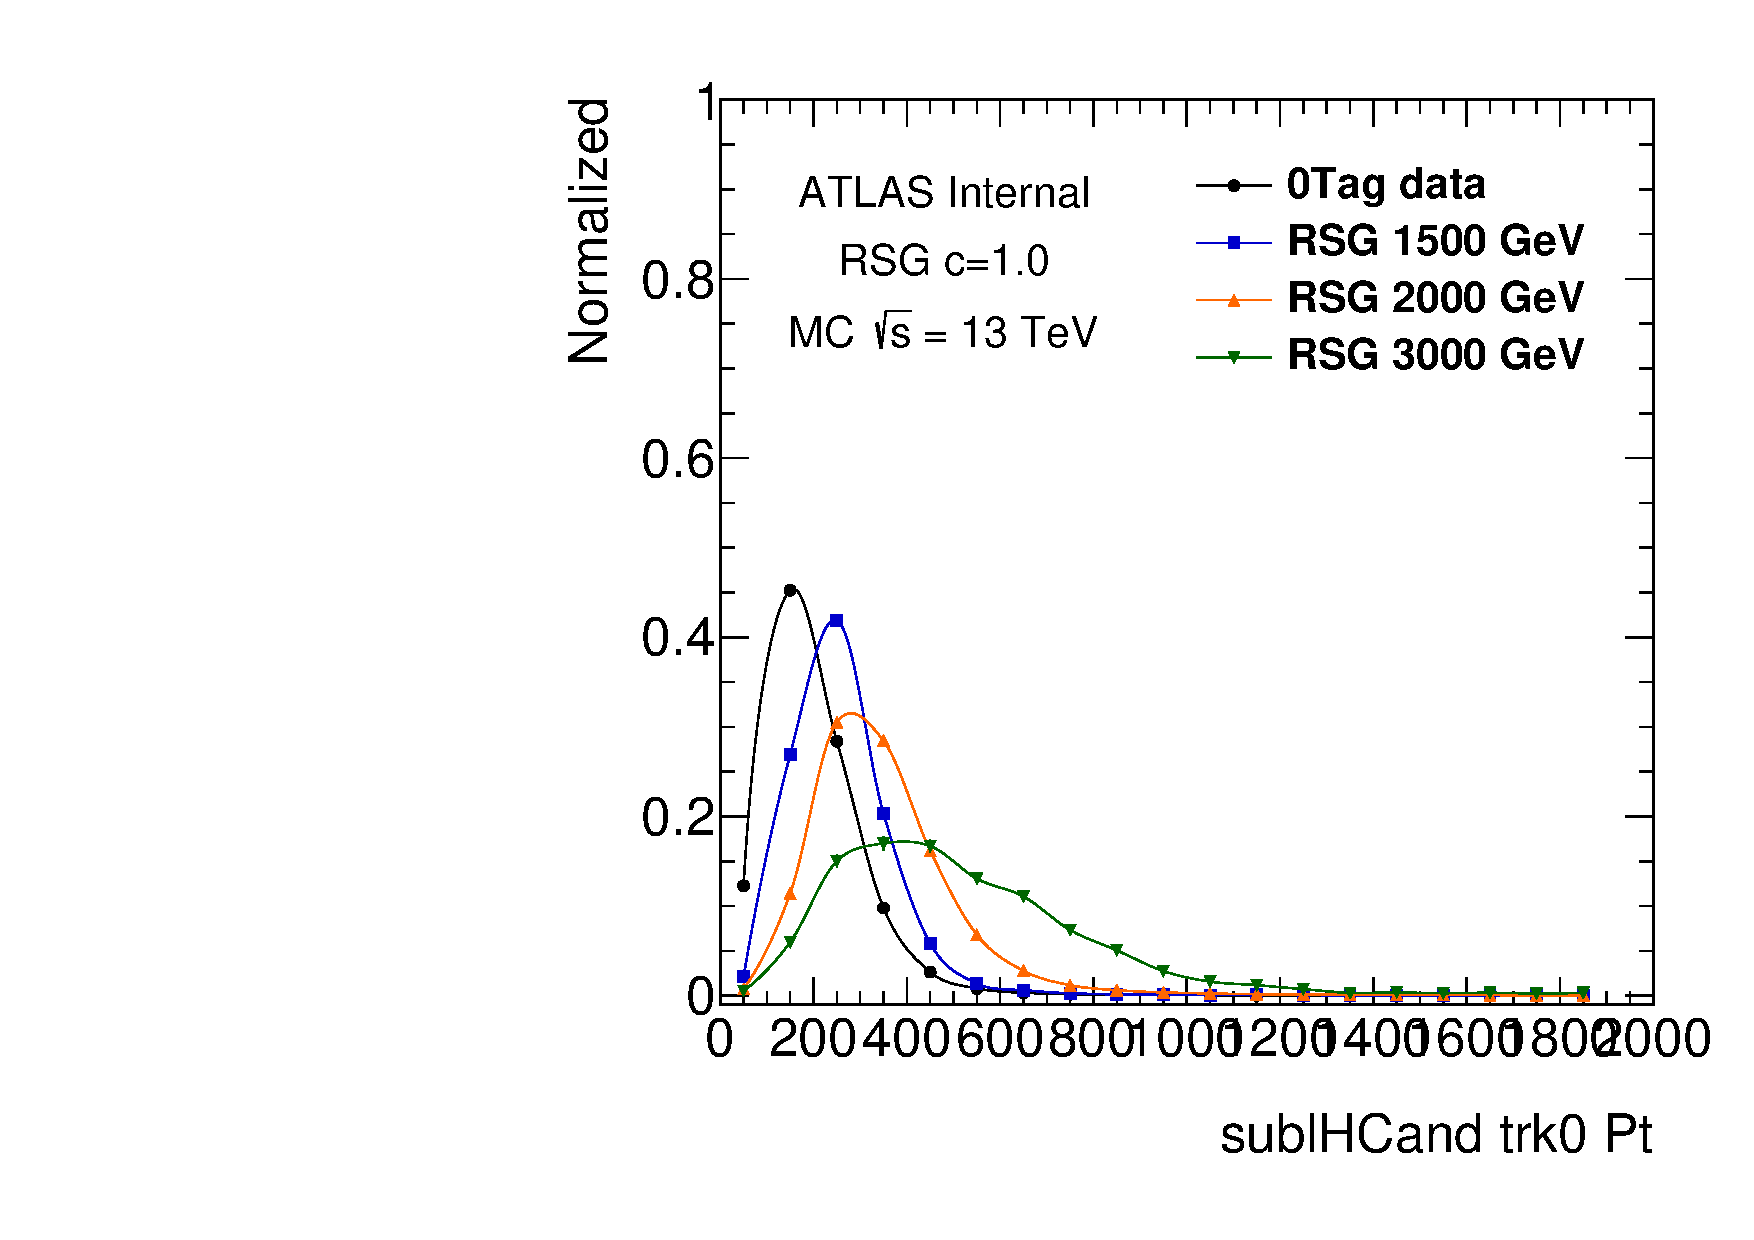
\includegraphics[width=0.32\textwidth,angle=-90]{figures/boosted/Truth/Moriond_comp_0_ThreeTag_Signal_sublHCand_trk0_Pt.pdf}
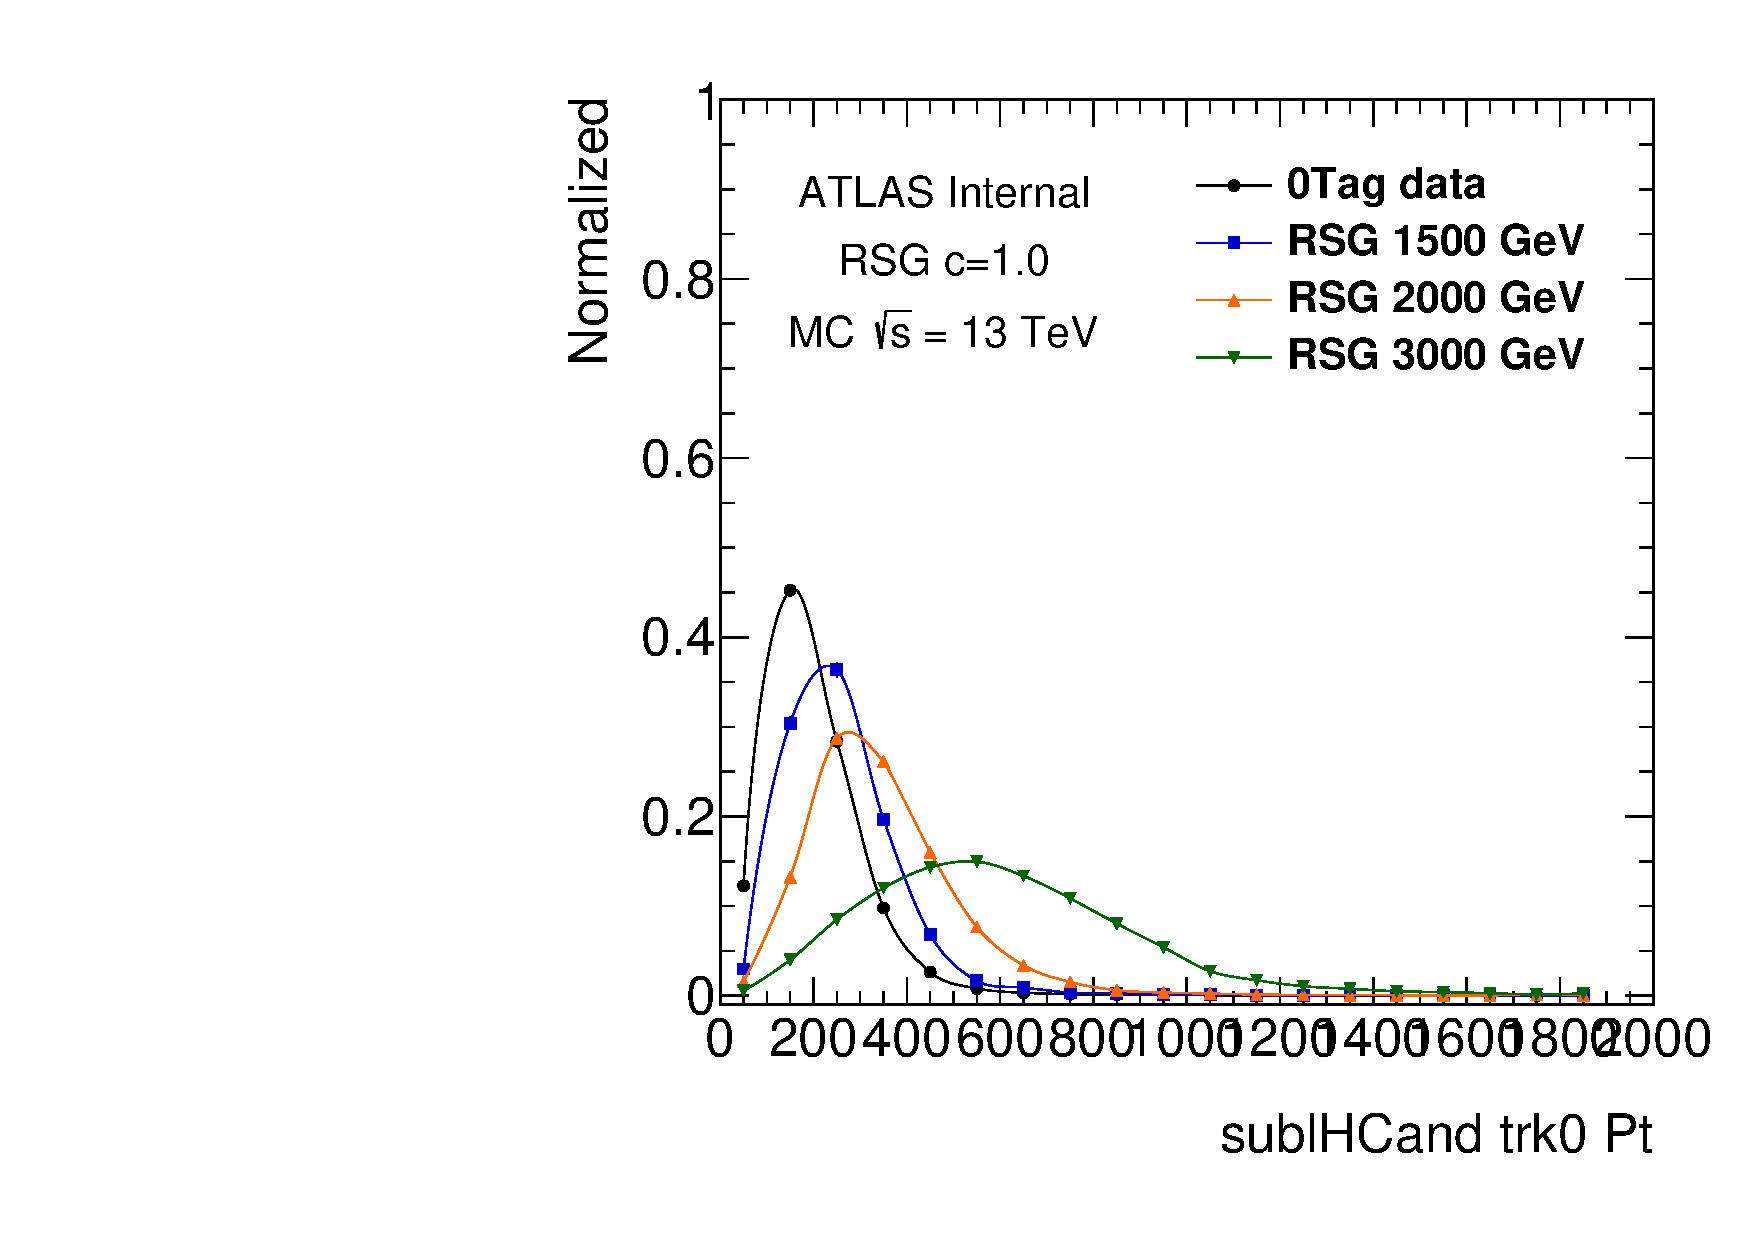
\includegraphics[width=0.32\textwidth,angle=-90]{figures/boosted/Truth/Moriond_comp_0_TwoTag_split_Signal_sublHCand_trk0_Pt.pdf}\\
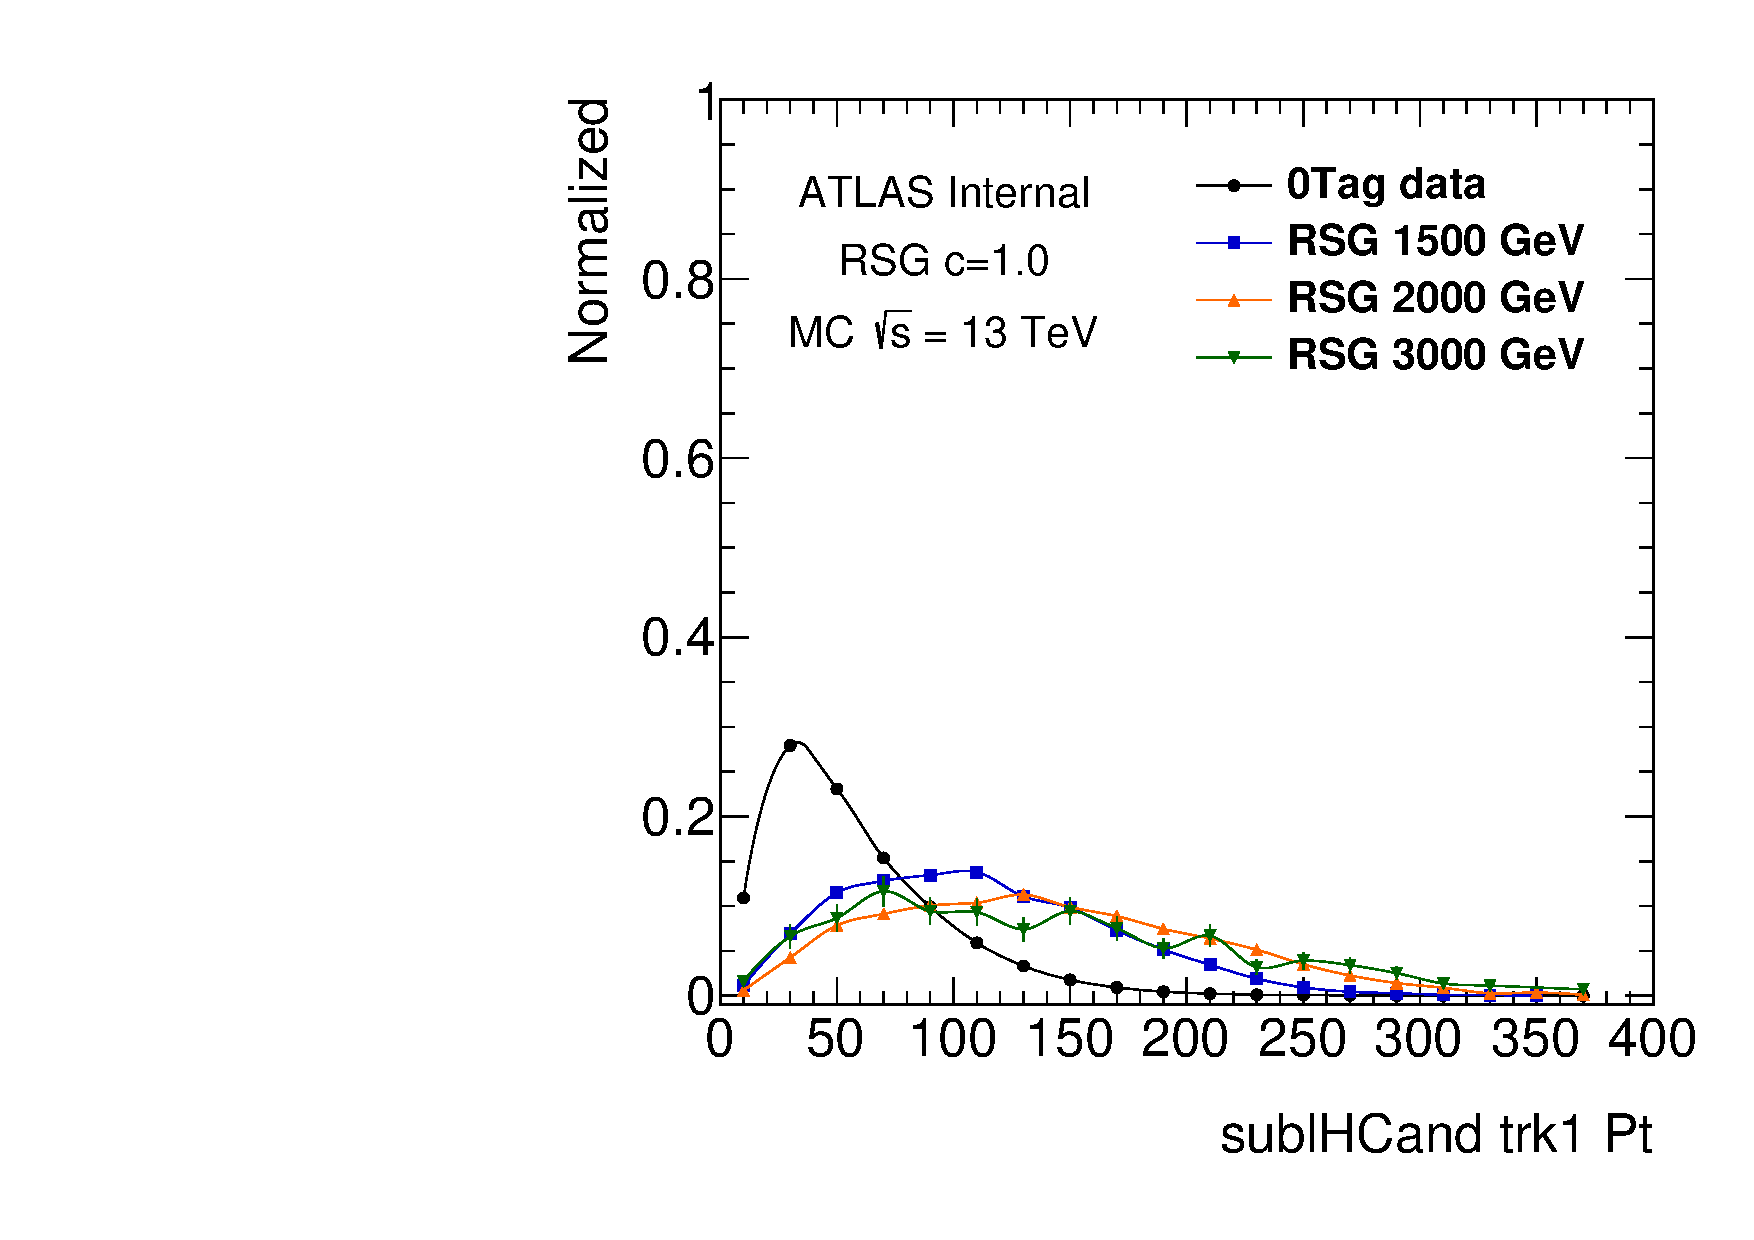
\includegraphics[width=0.32\textwidth,angle=-90]{figures/boosted/Truth/Moriond_comp_0_FourTag_Signal_sublHCand_trk1_Pt.pdf}
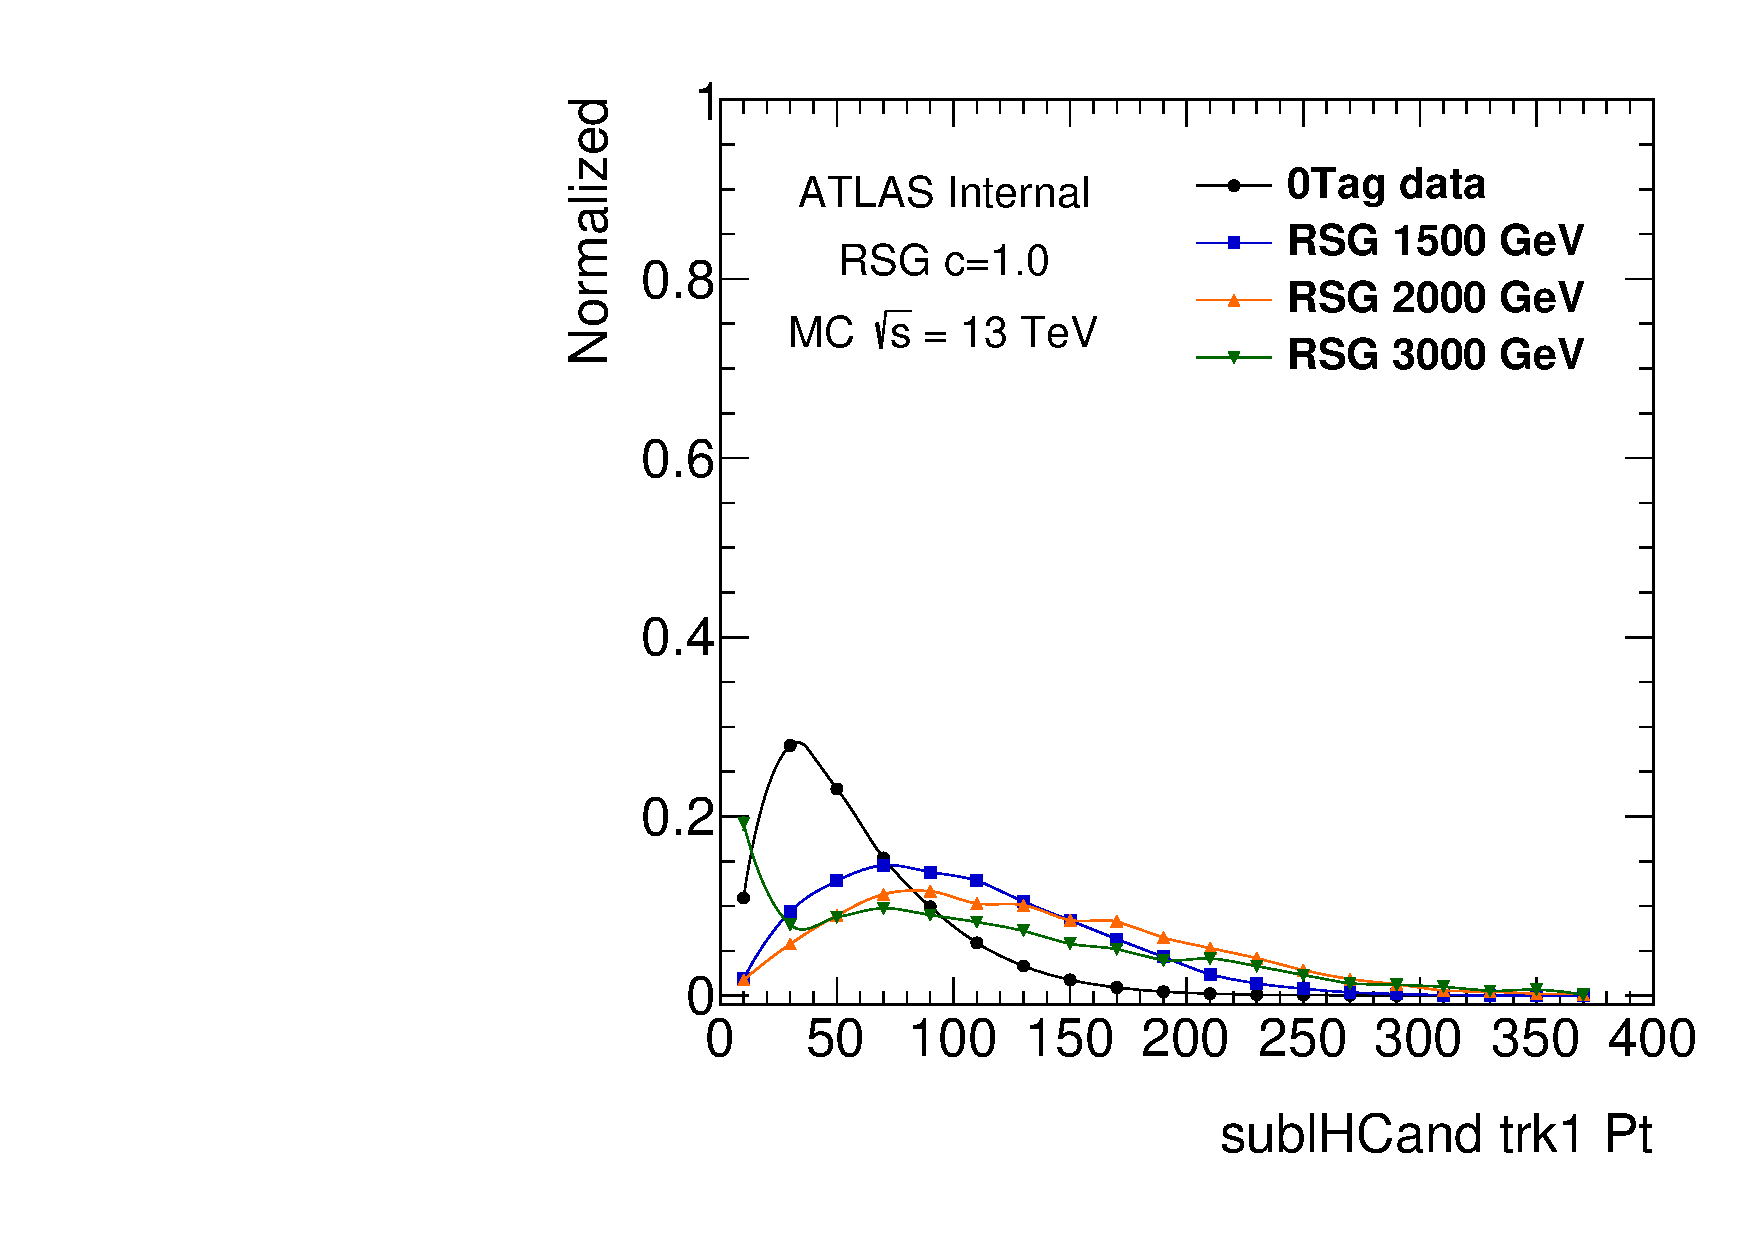
\includegraphics[width=0.32\textwidth,angle=-90]{figures/boosted/Truth/Moriond_comp_0_ThreeTag_Signal_sublHCand_trk1_Pt.pdf}
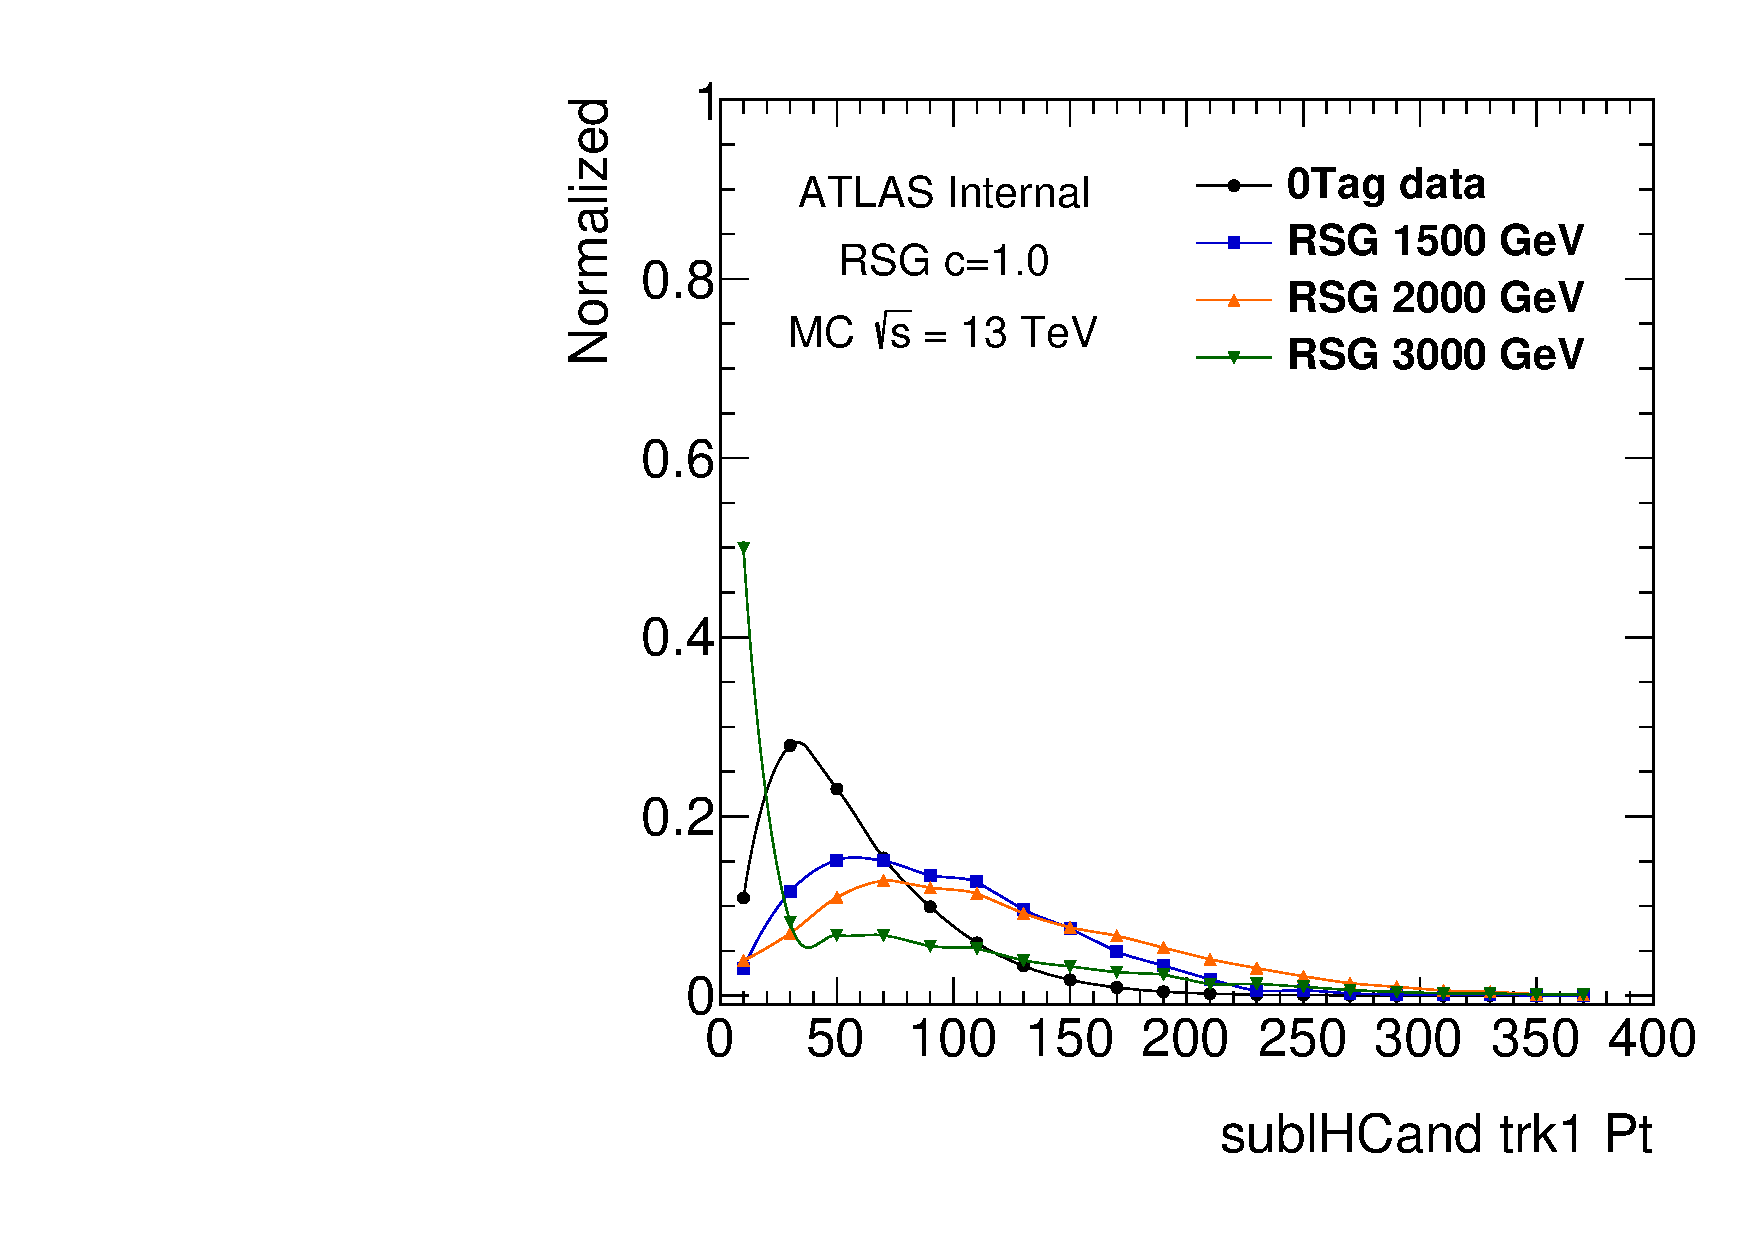
\includegraphics[width=0.32\textwidth,angle=-90]{figures/boosted/Truth/Moriond_comp_0_TwoTag_split_Signal_sublHCand_trk1_Pt.pdf}\\
\caption{For RSG $c=1.0$ samples, the subleading higgs candidate's $p_T$, mass, leading track jet $p_T$ and subleading trackjet $p_T$. The left column is $4b$, the middle column is $3b$, and the right column is $2bs$.}
\label{fig:app-signal-sublHCand}
\end{center}
\end{figure*}
